\chapter{DTC training and testing plots}
\label{app:DTC-plots}
This appendix collects the plots of the final \ac{DTC} trainings ($\gamma = 1000$, $K = 2$) that are not shown in Sec.~\ref{subsec:train-test-DTC}. For each distance metric and for the two detectors. As in the main text, the cluster with the largest number of events in the \ac{DEP} is drawn with the colour of the metric and the other one in grey.

\section{V08682A}
 Figs.~\ref{fig:acf-training}-\ref{fig:cid-training} show the reconstruction of a fixed validation waveform at different epochs together with the evolution of the training and validation losses, while Figs.~\ref{fig:acf-aoe}-\ref{fig:cid-aoe} show the clustering results and the \ac{AE} and rise time distributions of the two clusters for the validation and test sets.
%==================================================
% Reconstruction and losses
%==================================================

\begin{figure}[H]
    \centering
    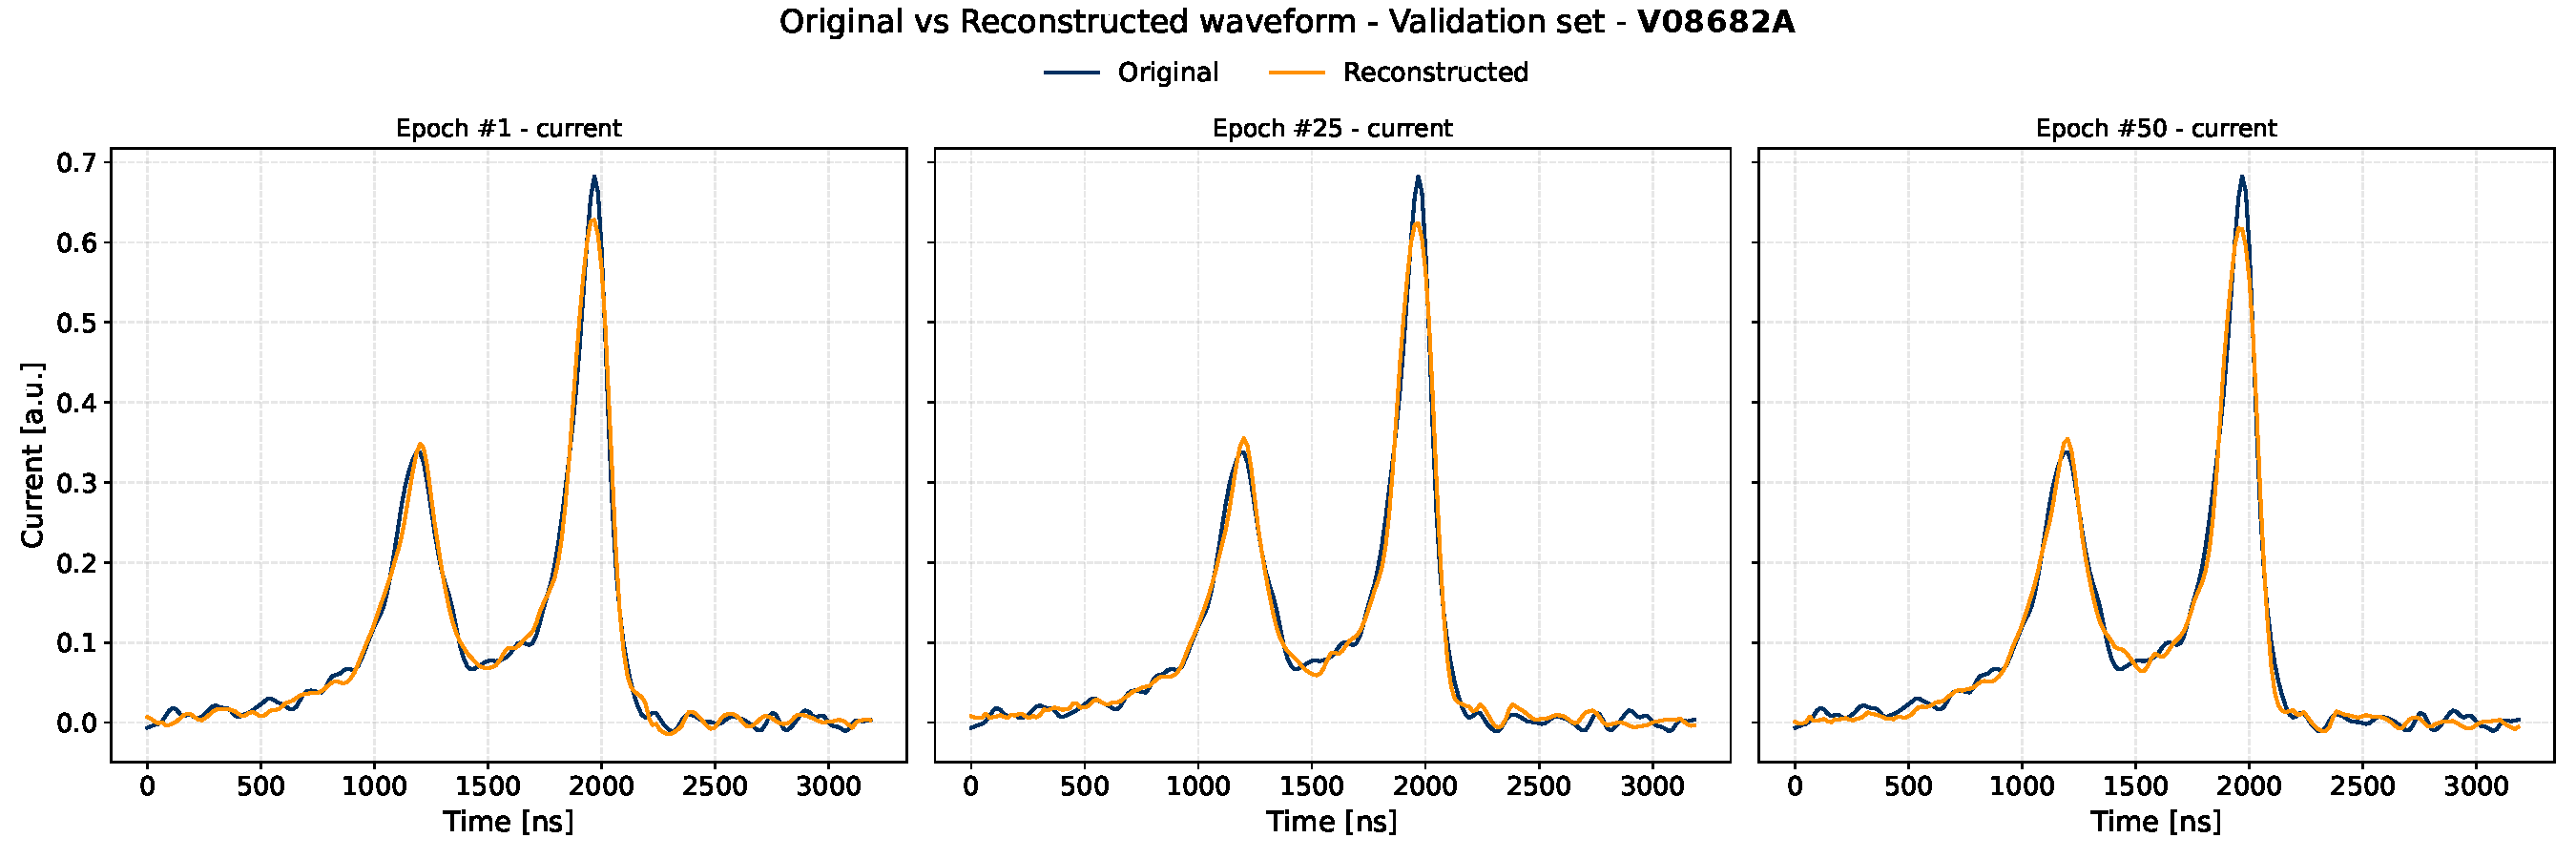
\includegraphics[width=\textwidth,height=0.36\textheight,keepaspectratio]{plots/DTC/acf/acf_2cl_training_reconstruction.pdf}\\[4pt]
    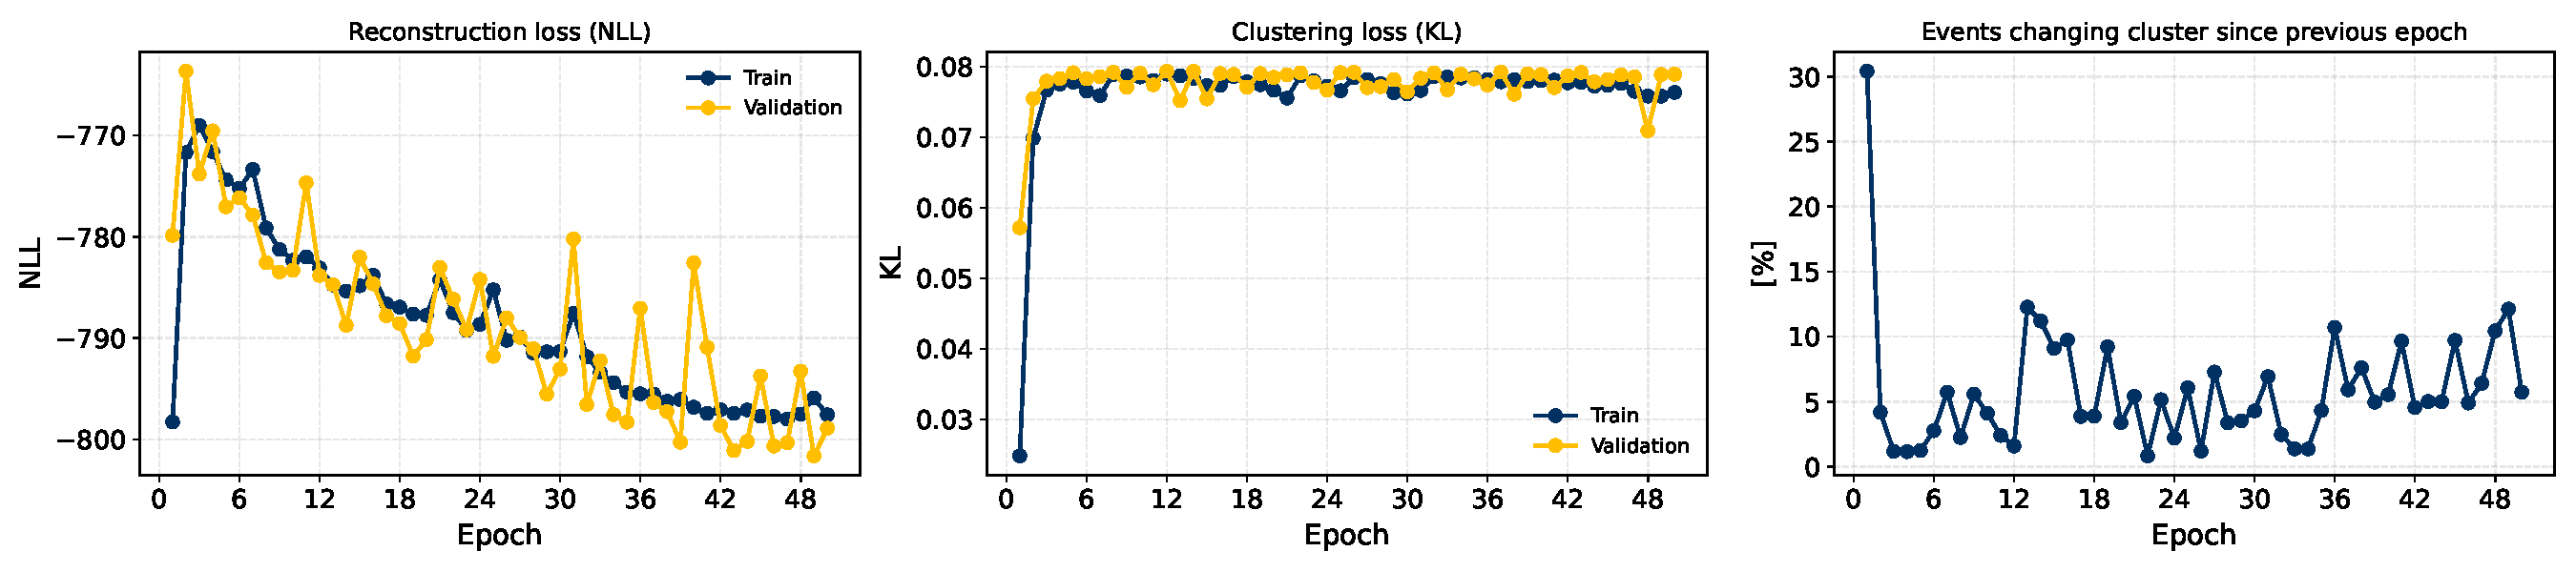
\includegraphics[width=\textwidth,height=0.36\textheight,keepaspectratio]{plots/DTC/acf/acf_2cl_training_history.pdf}
    \caption{Reconstructed waveforms through epochs (top), losses and fraction of events changing cluster per epoch (bottom) with the \ac{ACF} metric - V08682A.}
    \label{fig:acf-training}
    \label{fig:acf-reconstruction}
    \label{fig:acf-losses}
\end{figure}

\begin{figure}[H]
    \centering
    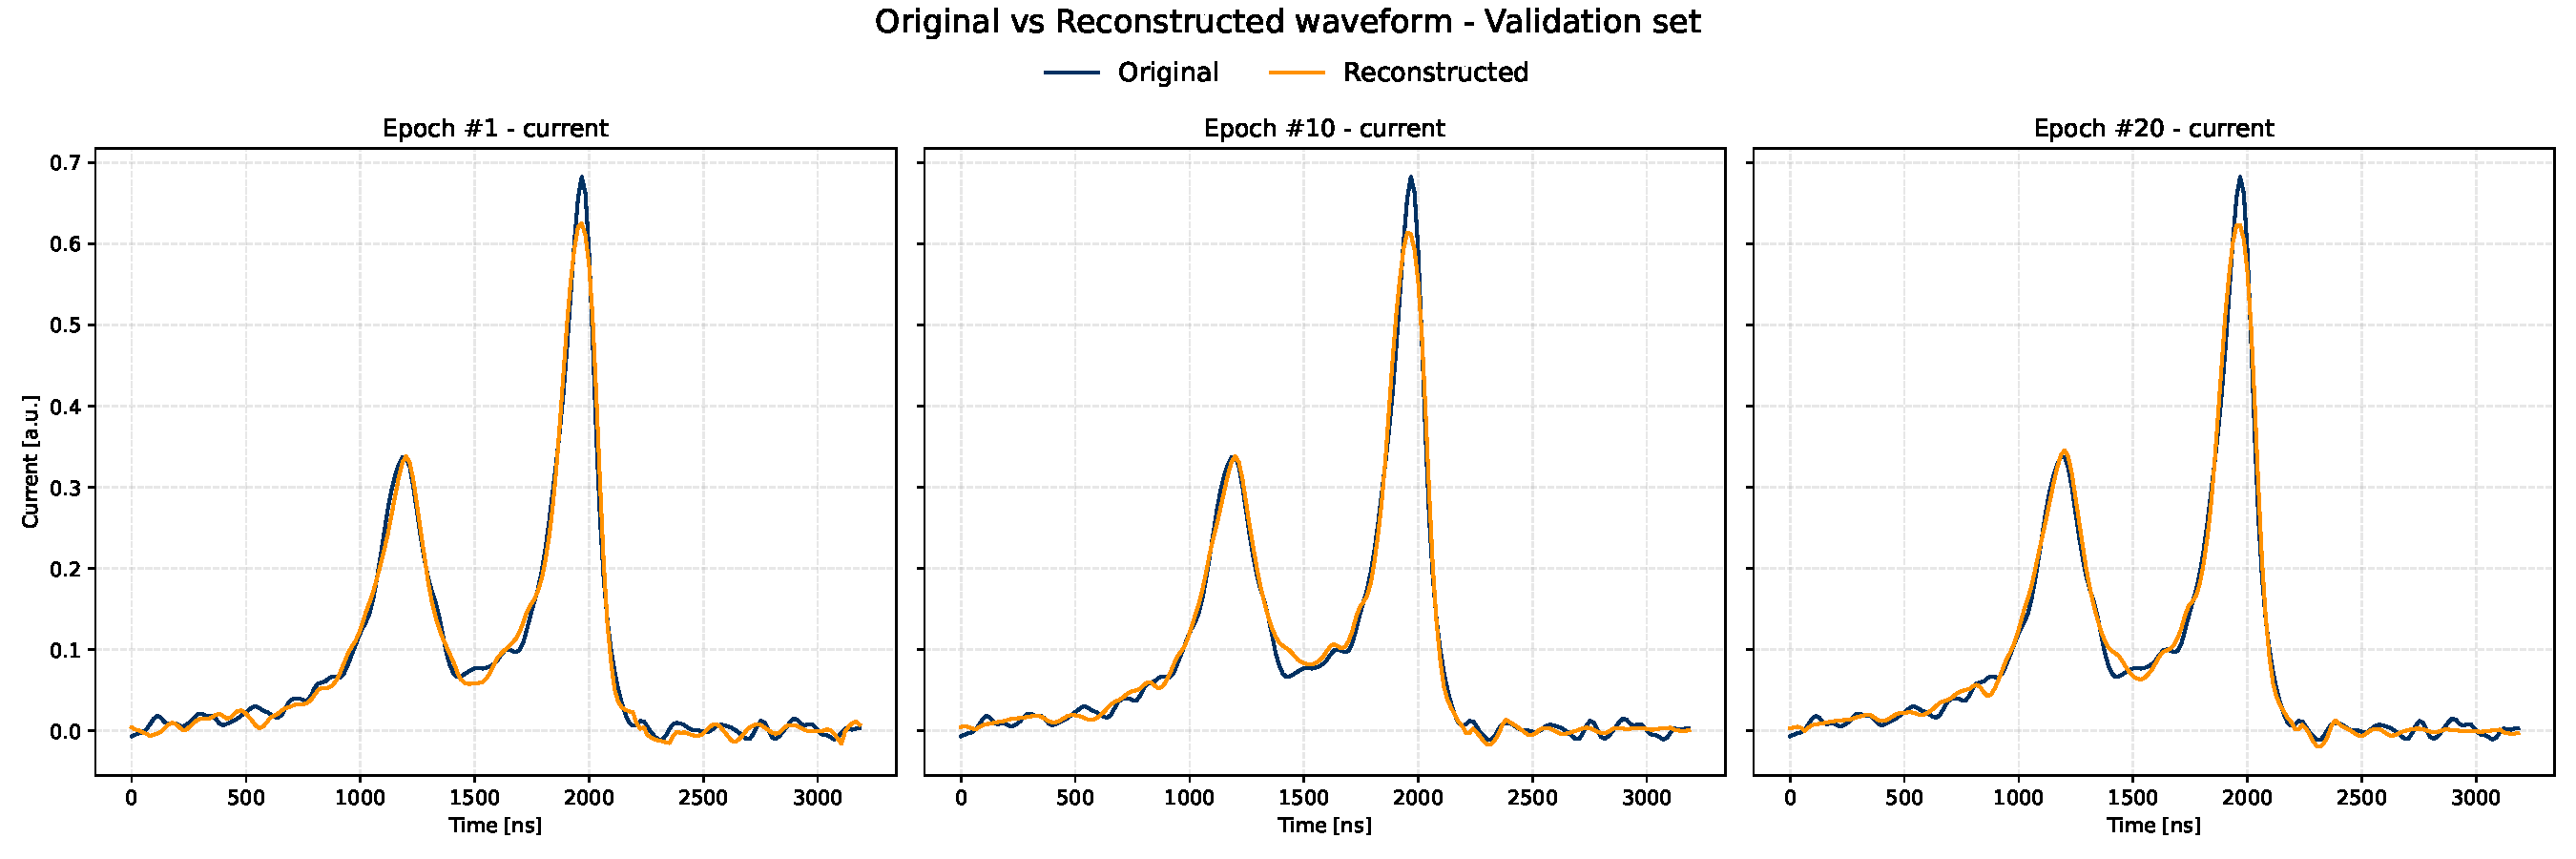
\includegraphics[width=\textwidth,height=0.36\textheight,keepaspectratio]{plots/DTC/euclidean/eucl_2cl_training_reconstruction.pdf}\\[4pt]
    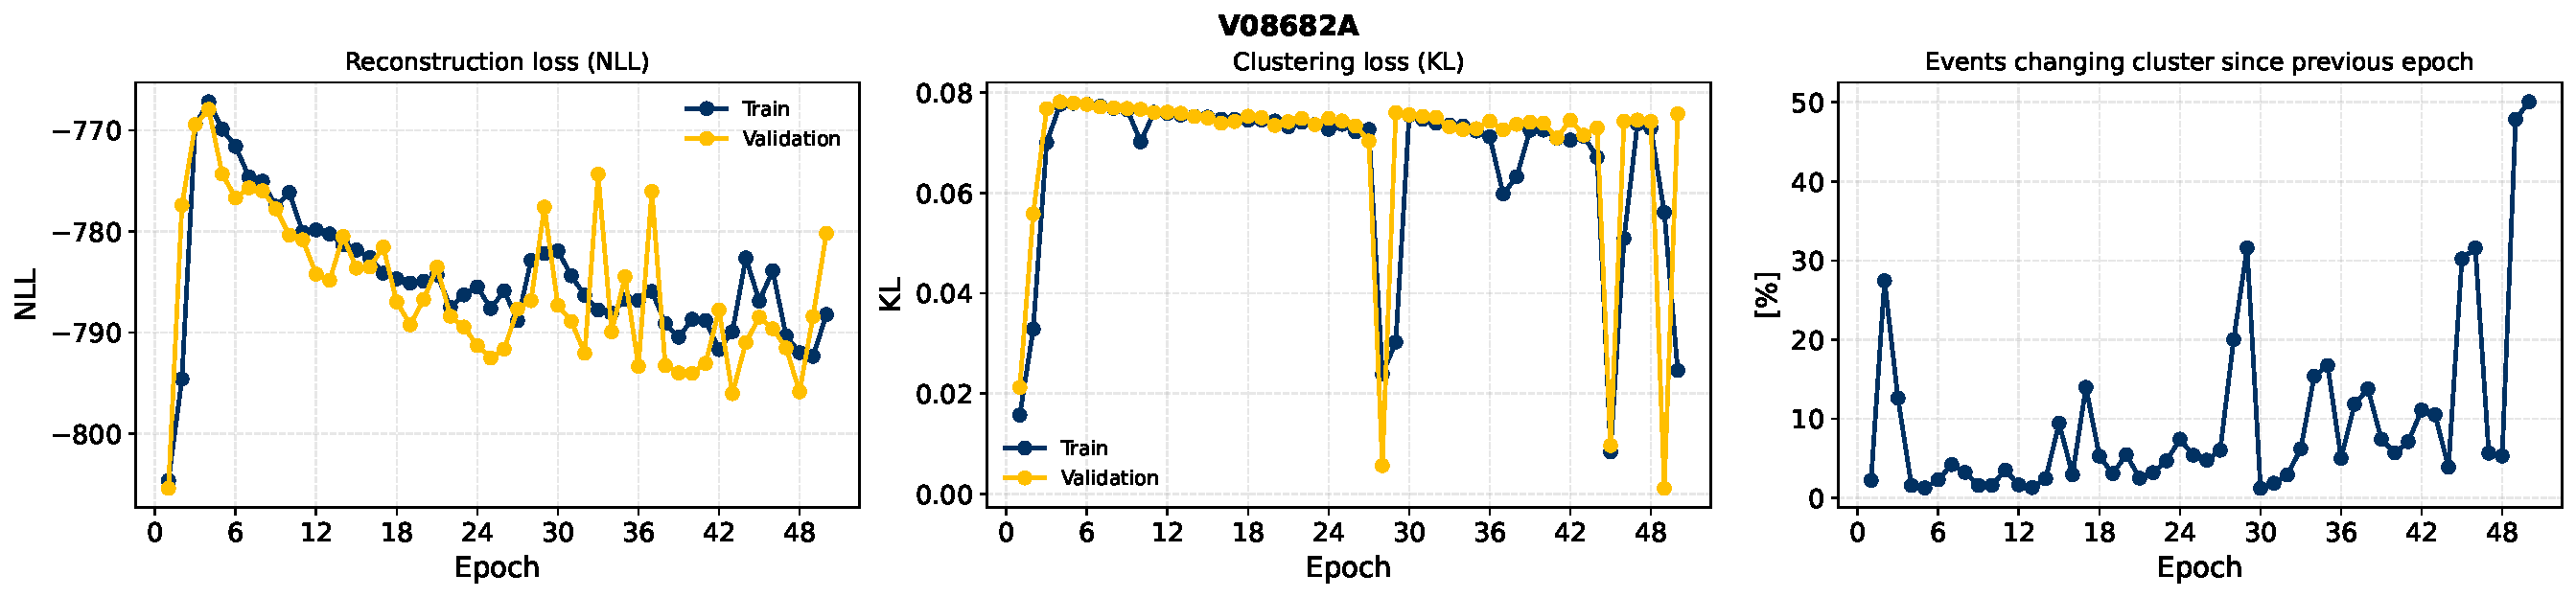
\includegraphics[width=\textwidth,height=0.36\textheight,keepaspectratio]{plots/DTC/euclidean/eucl_2cl_training_history.pdf}
    \caption{Reconstructed waveforms through epochs (top), losses and fraction of events changing cluster per epoch (bottom) with the \ac{EUC} metric - V08682A.}
    \label{fig:euclidean-training}
    \label{fig:euclidean-reconstruction}
    \label{fig:euclidean-losses}
\end{figure}

\begin{figure}[H]
    \centering
    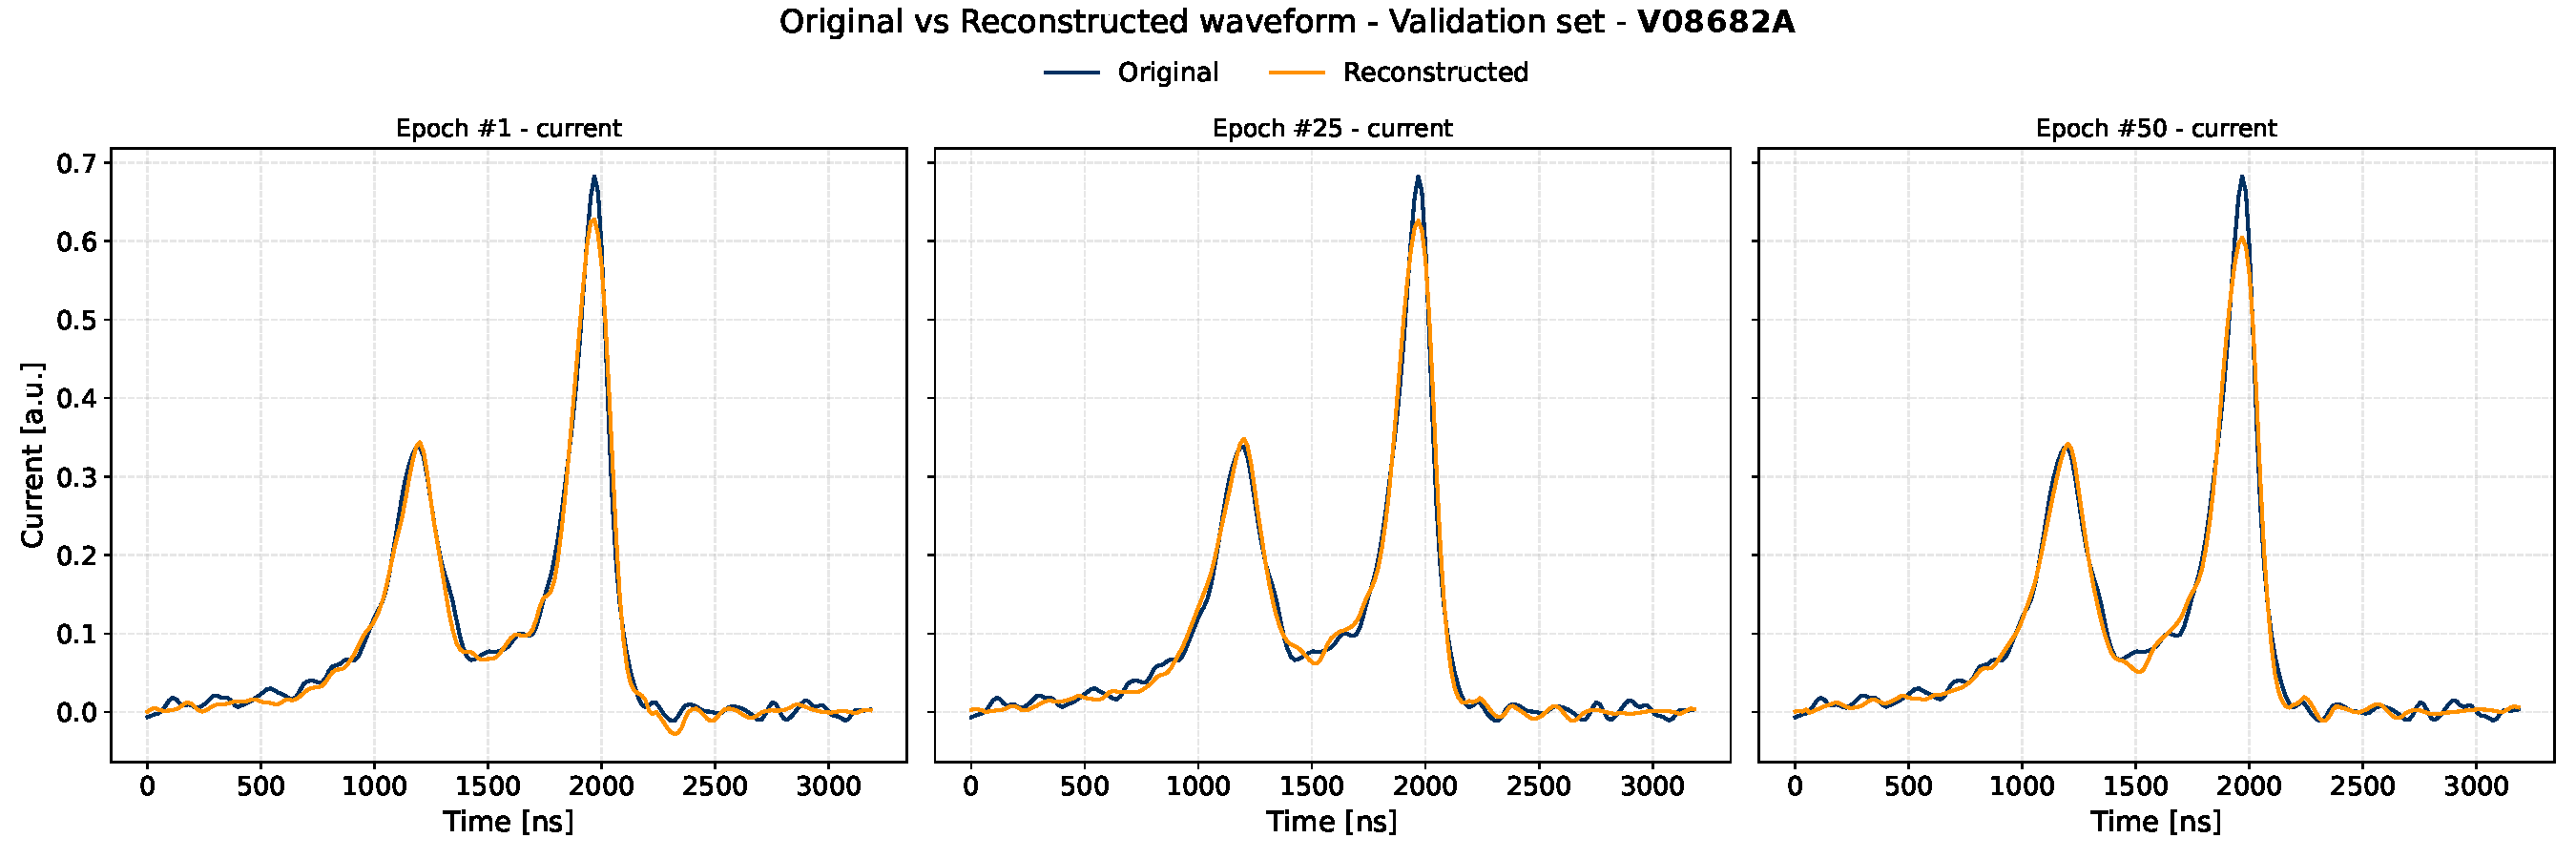
\includegraphics[width=\textwidth,height=0.36\textheight,keepaspectratio]{plots/DTC/cid/cid_2cl_training_reconstruction.pdf}\\[4pt]
    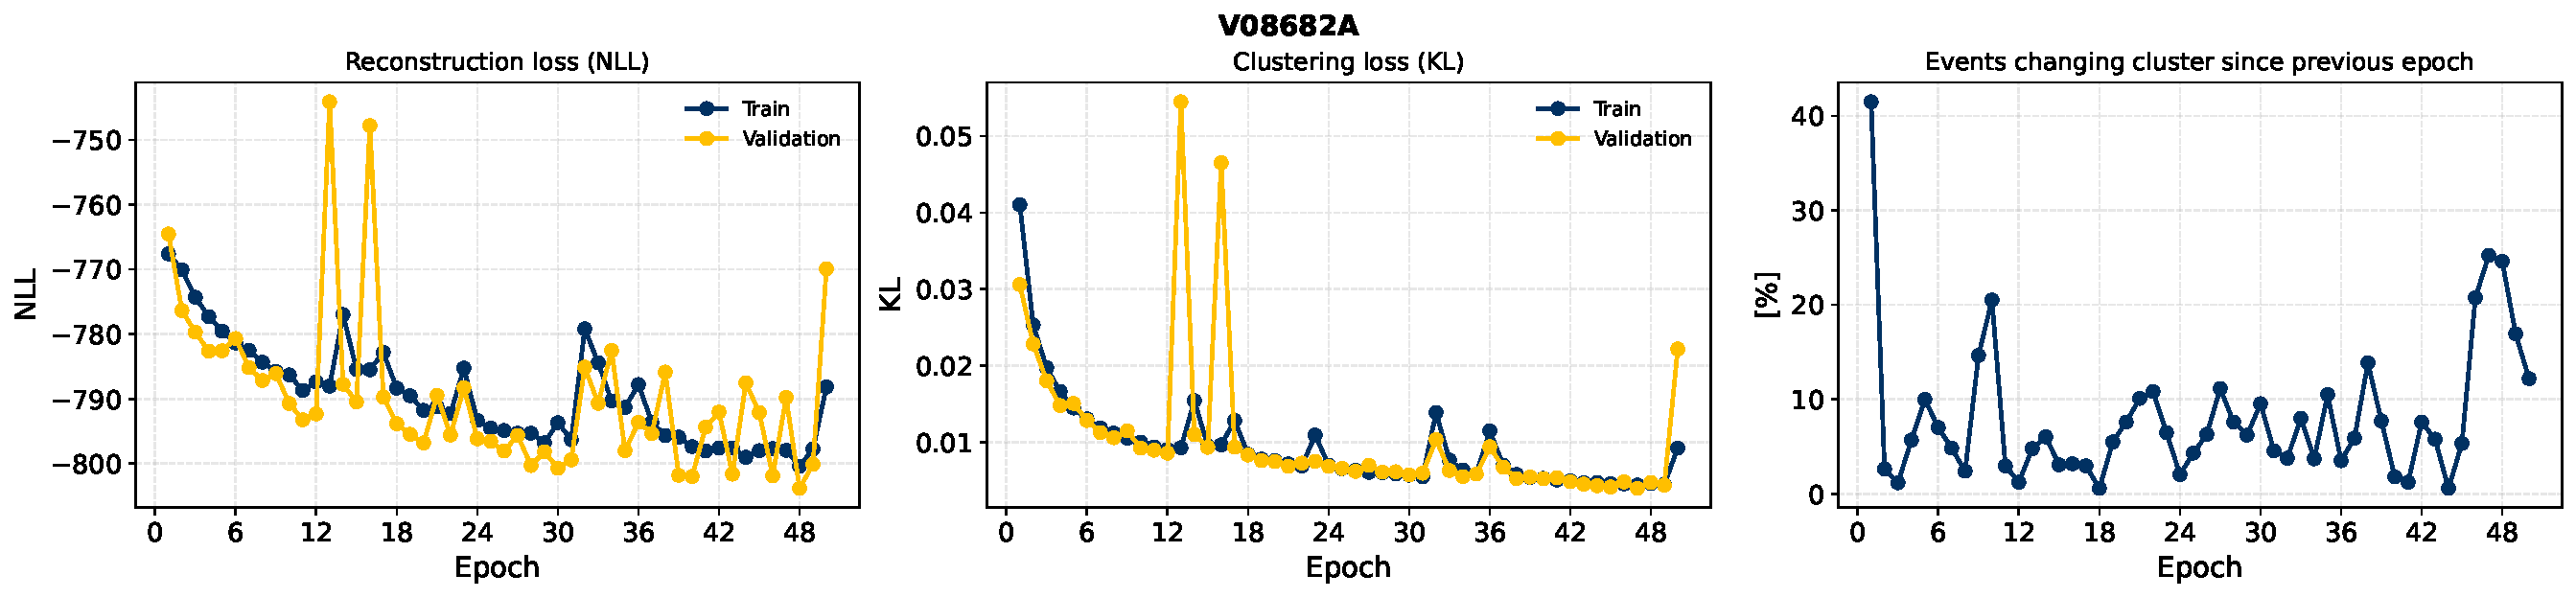
\includegraphics[width=\textwidth,height=0.36\textheight,keepaspectratio]{plots/DTC/cid/cid_2cl_training_history.pdf}
    \caption{Reconstructed waveforms through epochs (top), losses and fraction of events changing cluster per epoch (bottom) with the \ac{CID} metric - V08682A.}
    \label{fig:cid-training}
    \label{fig:cid-reconstruction}
    \label{fig:cid-losses}
\end{figure}

%==================================================
% Validation and test sets
%==================================================

\begin{figure}[H]
    \centering
    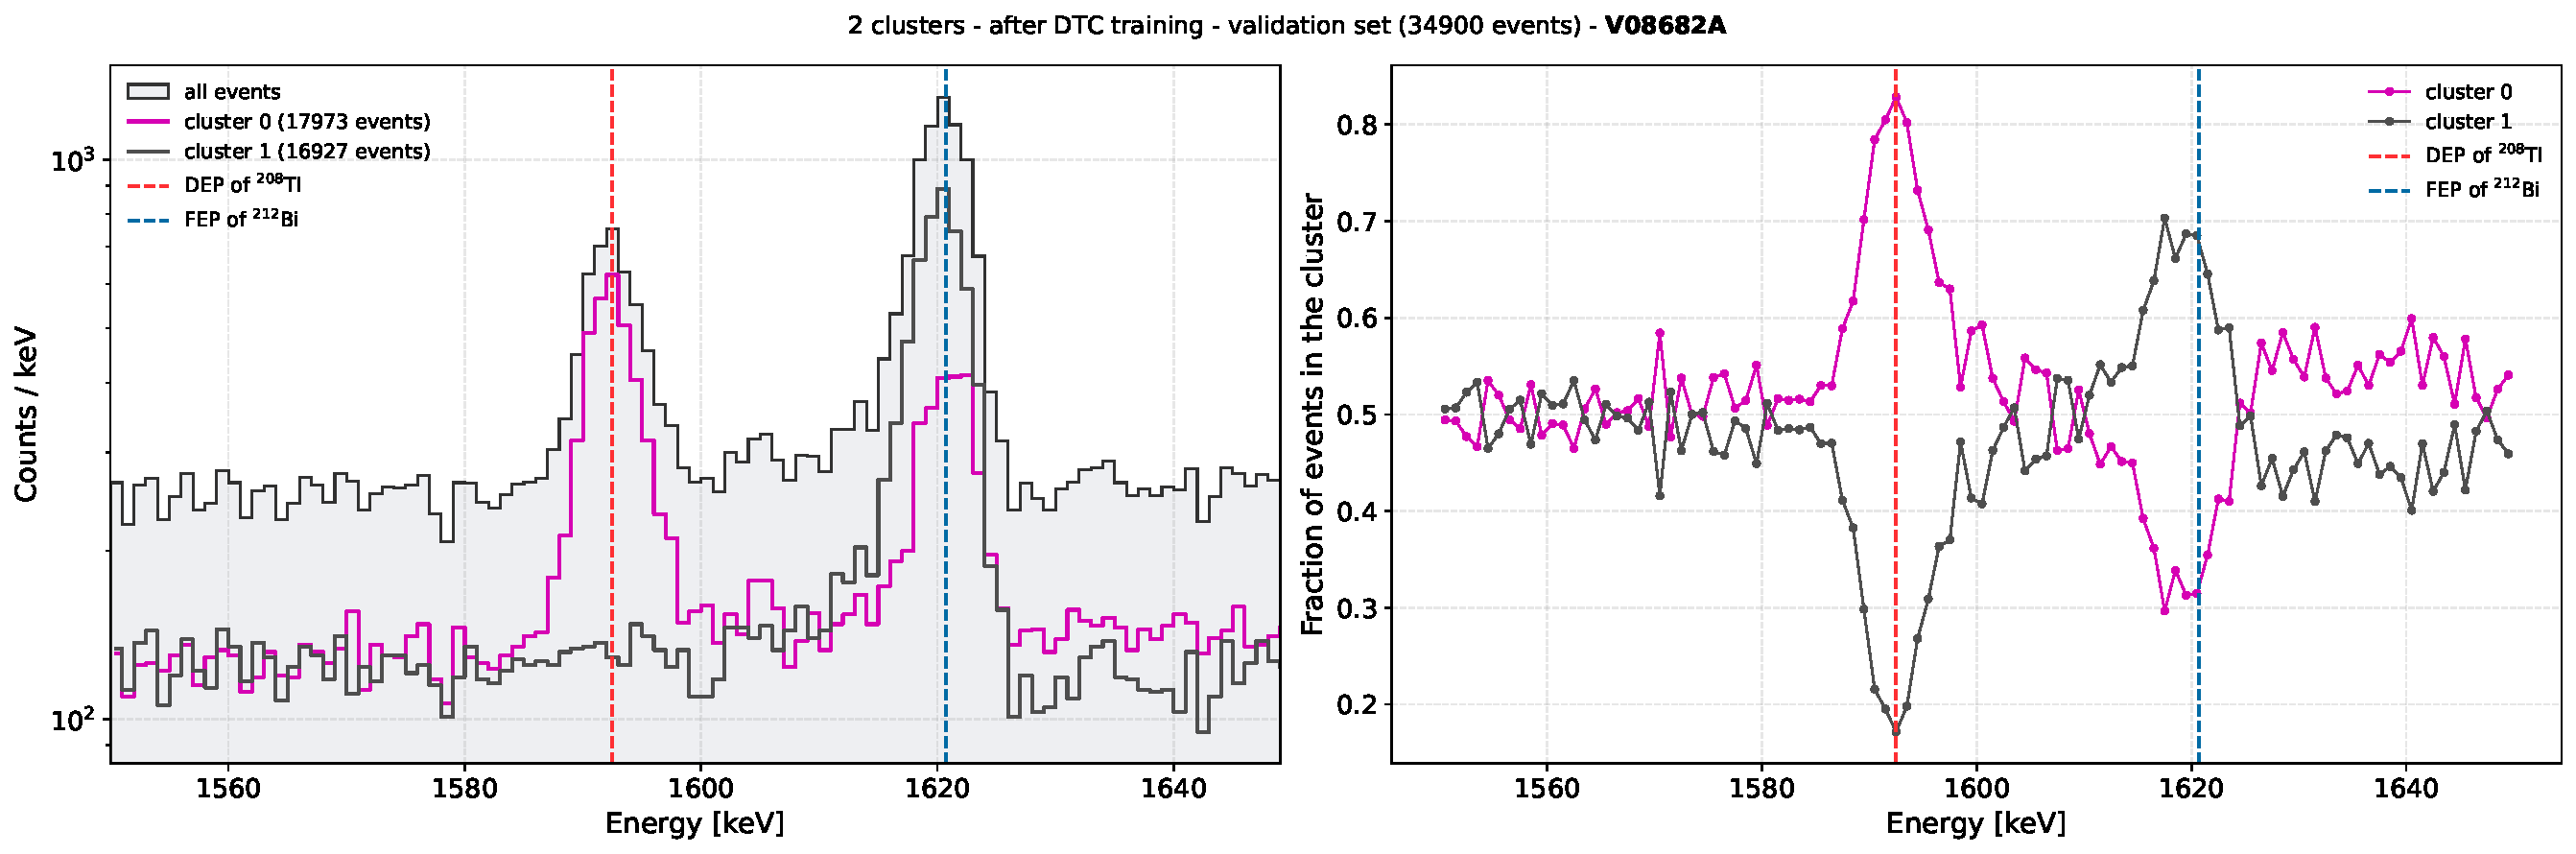
\includegraphics[width=\textwidth,height=0.27\textheight,keepaspectratio]{plots/DTC/acf/acf_2cl_energy_val.pdf}\\[2pt]
    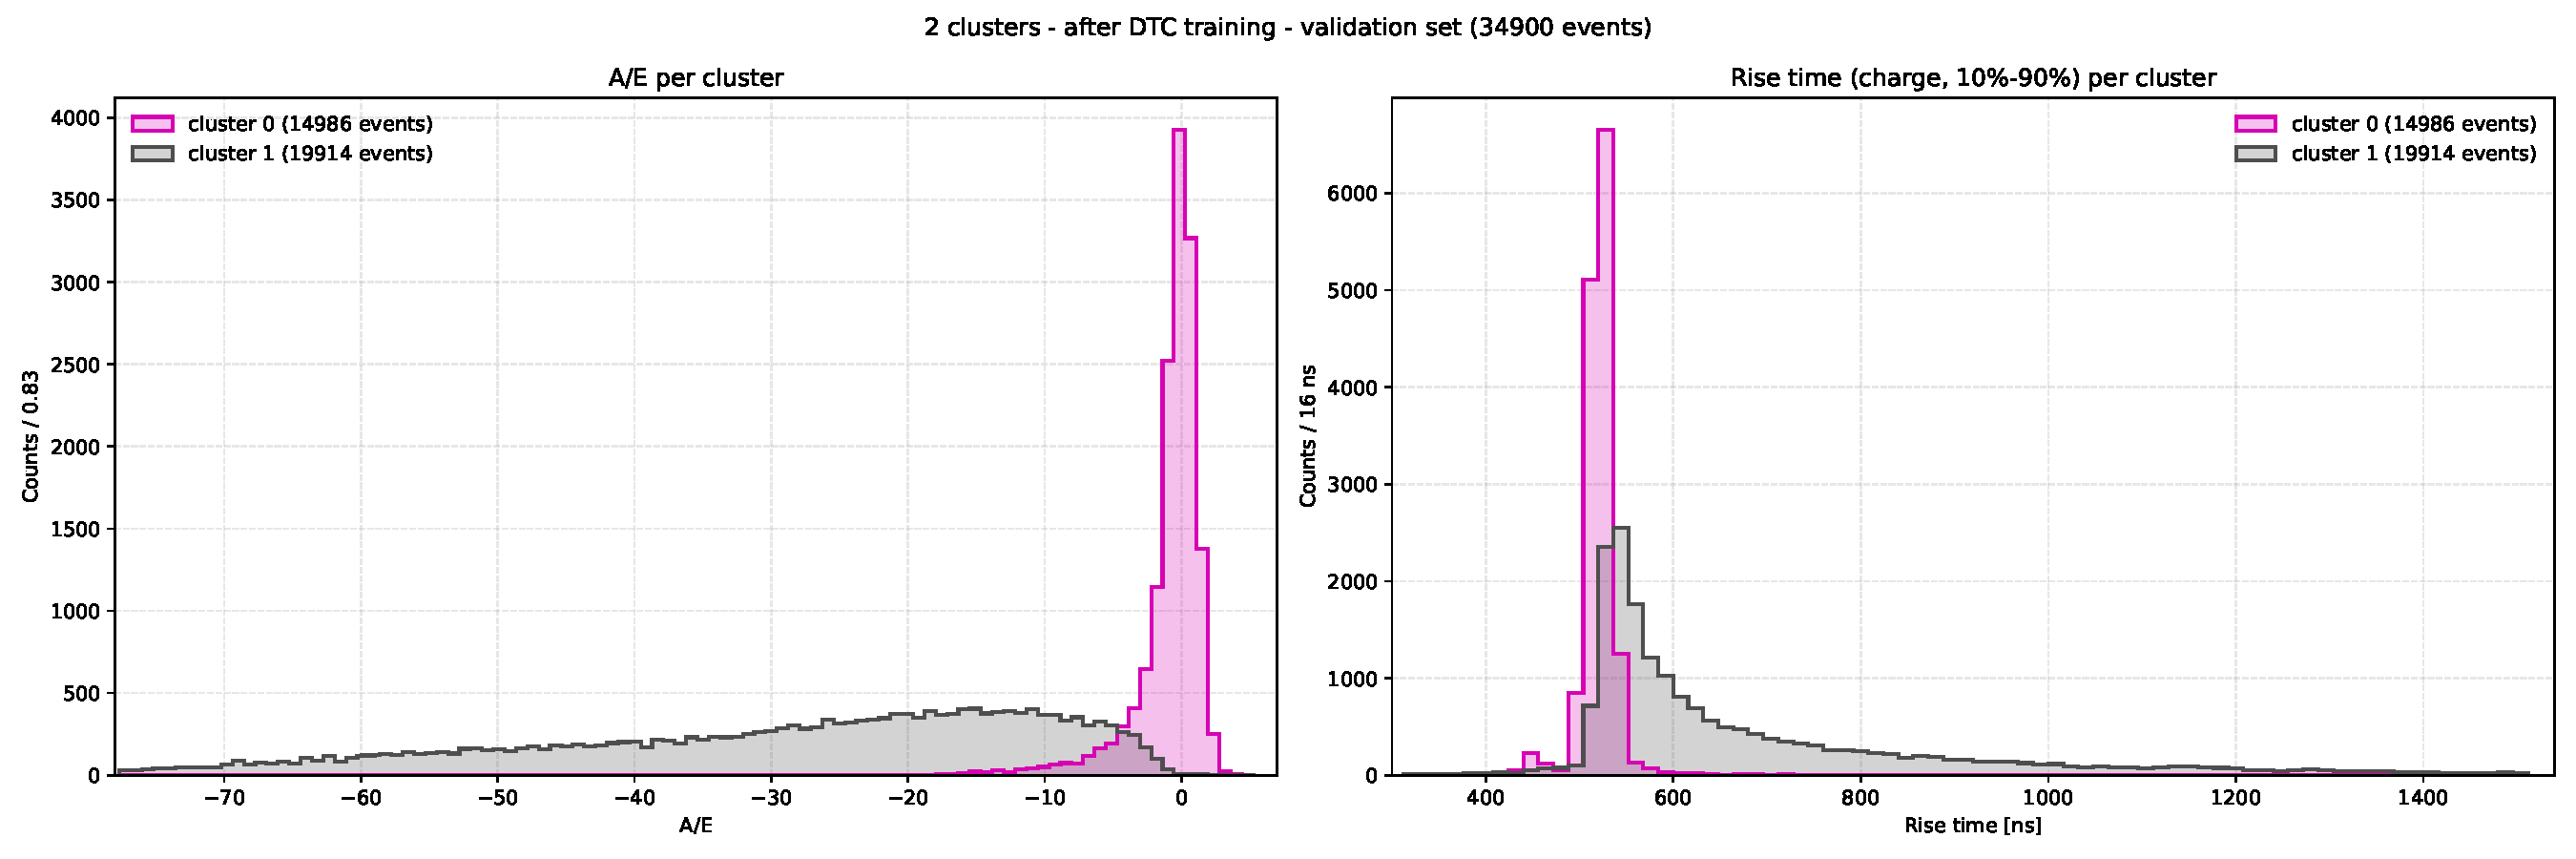
\includegraphics[width=\textwidth,height=0.27\textheight,keepaspectratio]{plots/DTC/acf/acf_2cl_AoE_risetime_val_linear.pdf}\\[2pt]
    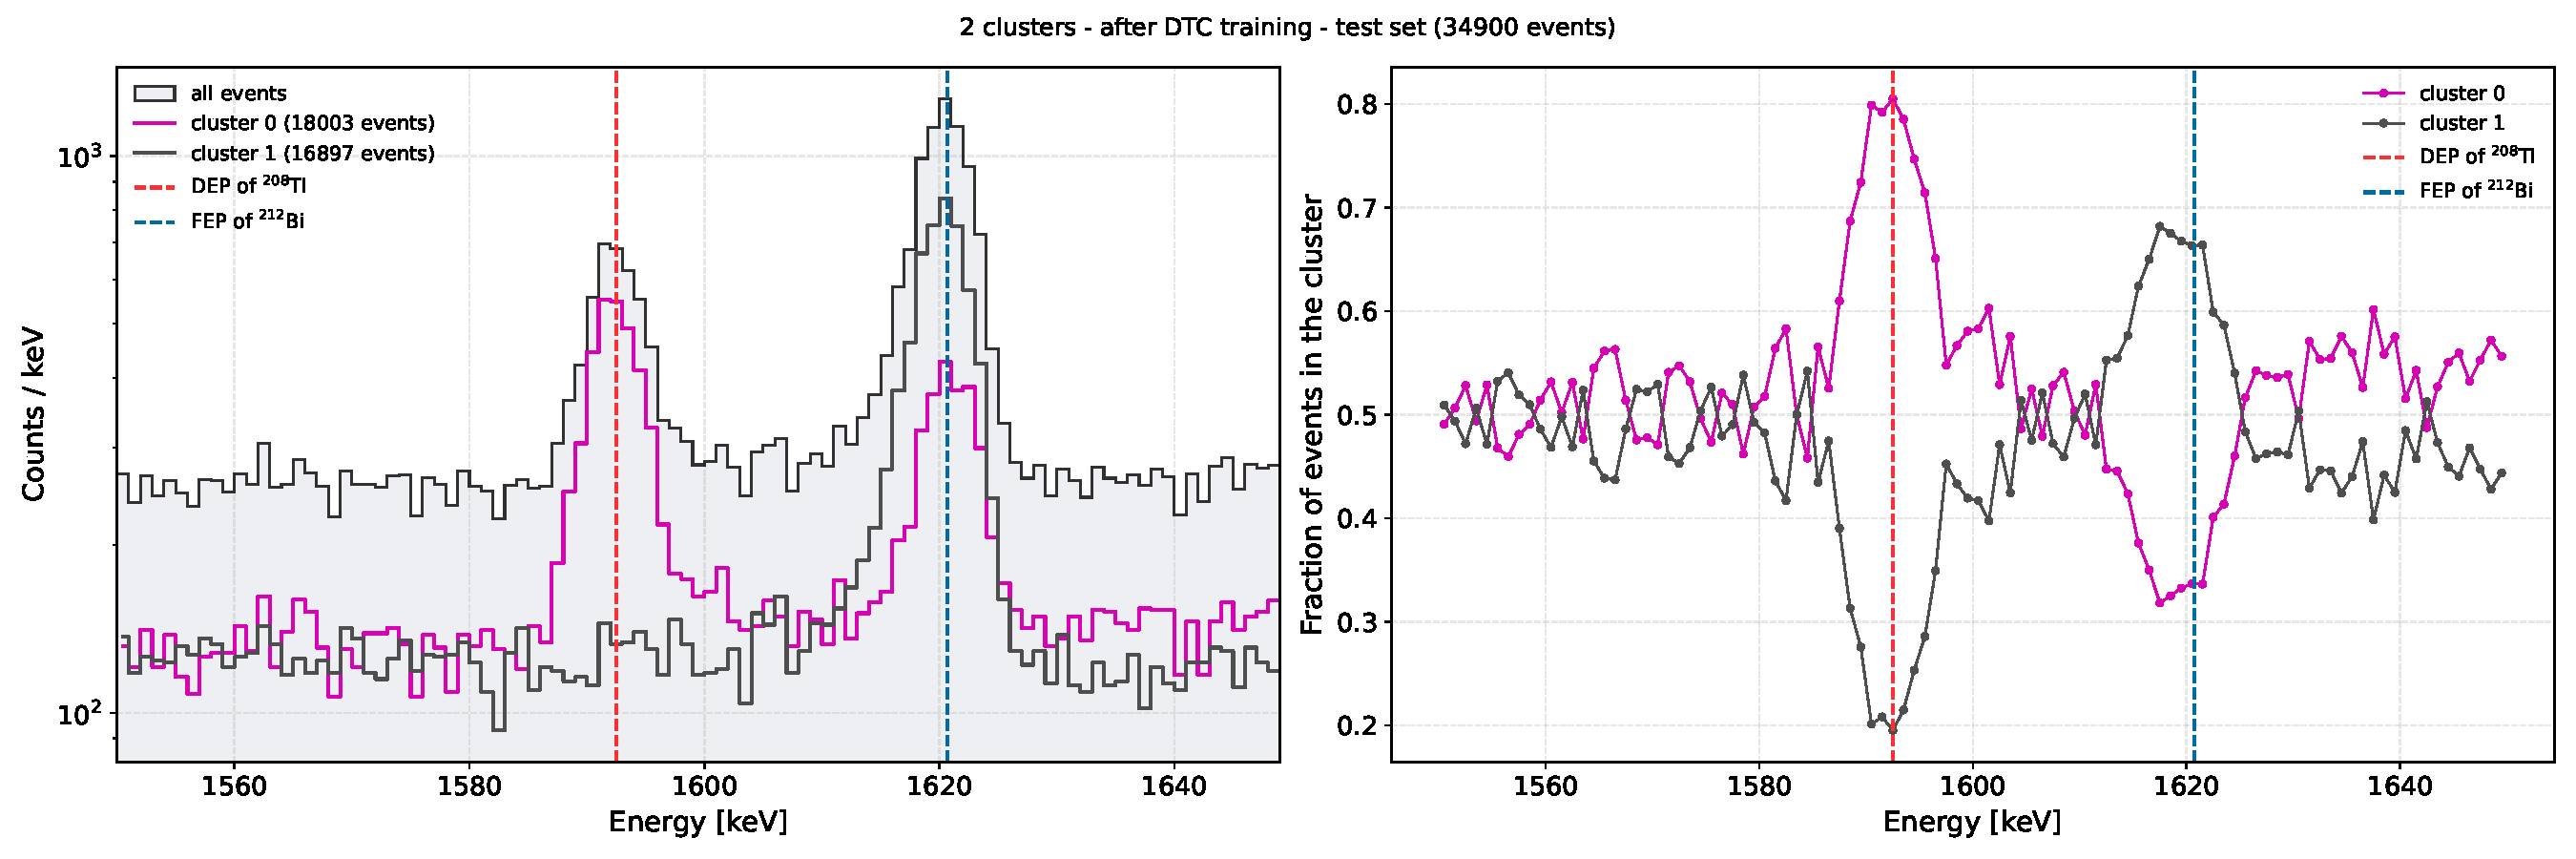
\includegraphics[width=\textwidth,height=0.27\textheight,keepaspectratio]{plots/DTC/acf/acf_2cl_energy_test.pdf}\\[2pt]
    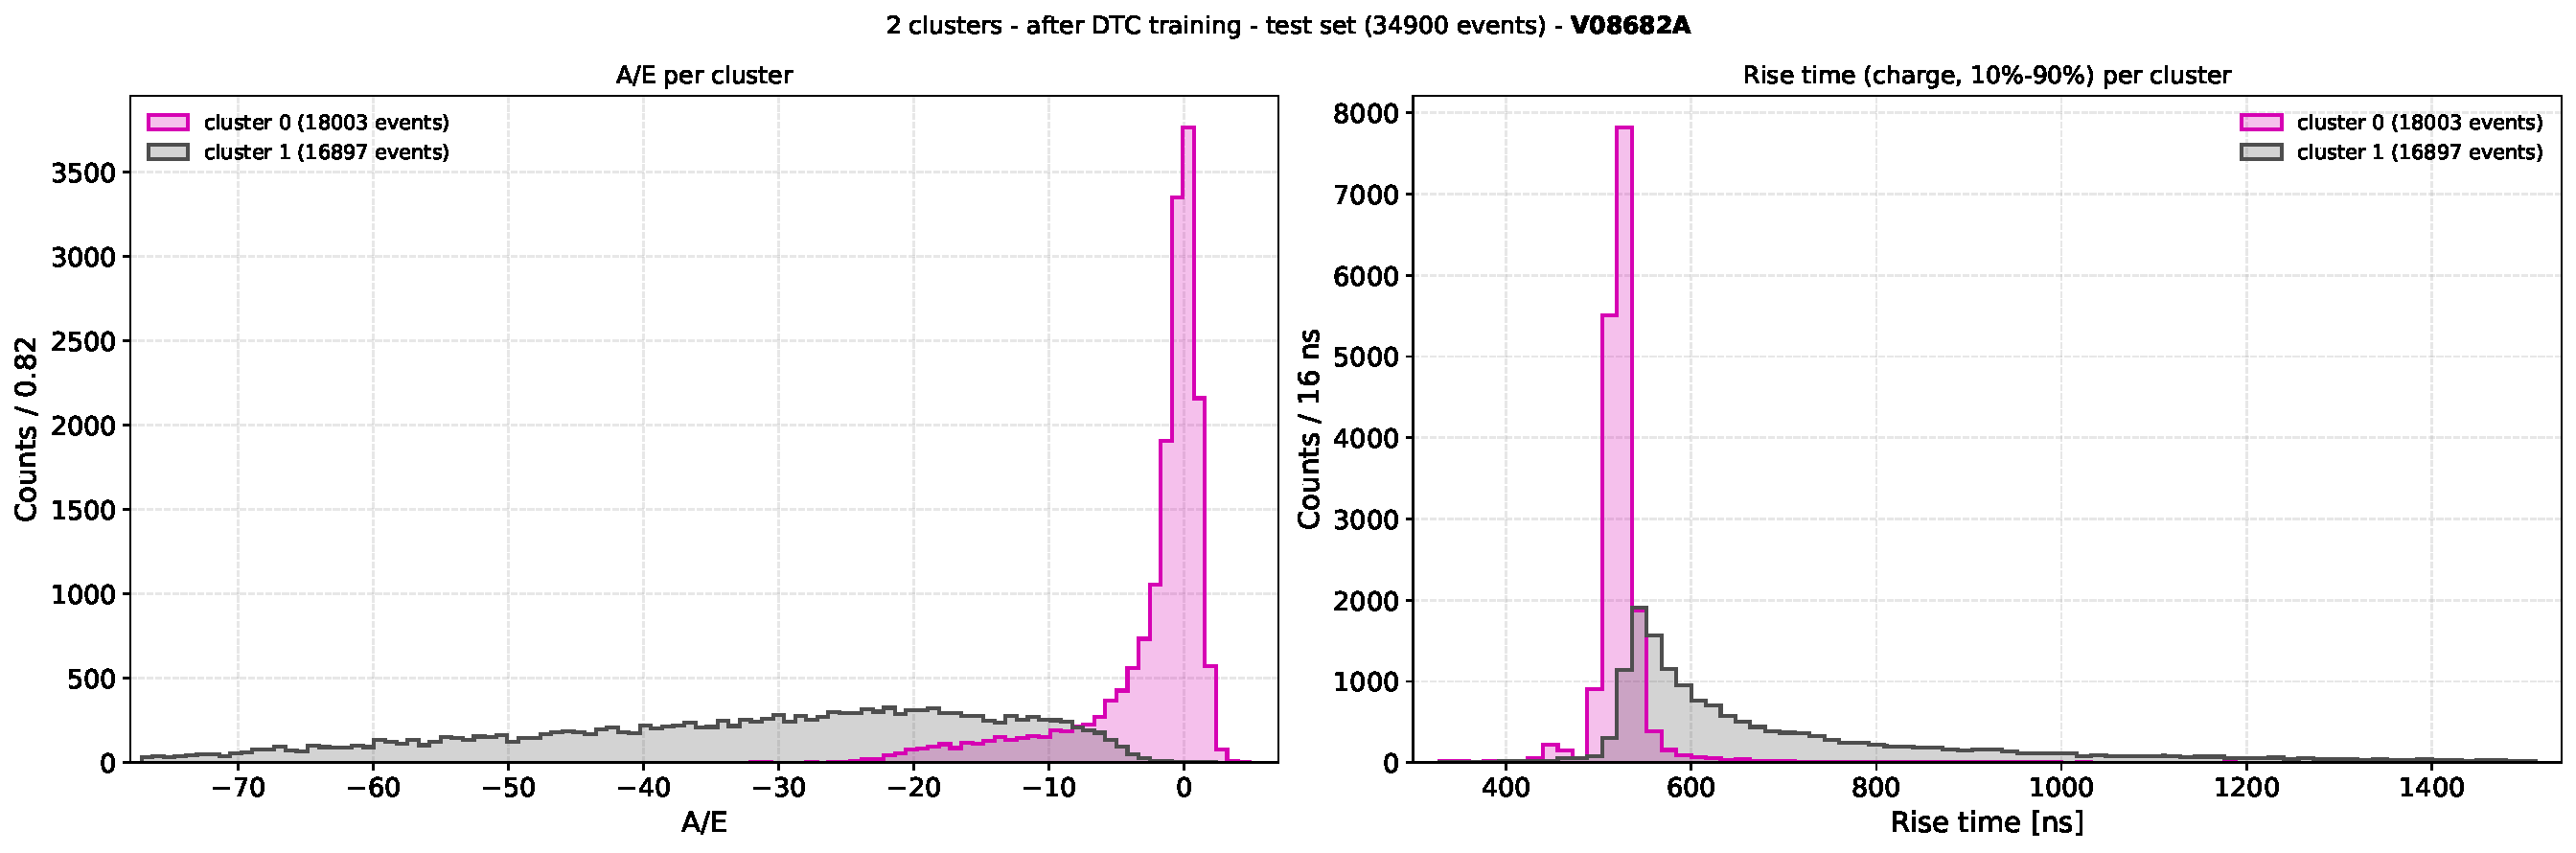
\includegraphics[width=\textwidth,height=0.27\textheight,keepaspectratio]{plots/DTC/acf/acf_2cl_AoE_risetime_test_linear.pdf}
    \caption{Clustering results with the \ac{ACF} metric on the validation set (first and second rows) and on the test set (third and fourth rows): energy spectrum of each cluster and fraction of events assigned to each cluster as a function of energy (first and third rows), and \ac{AE} and rise time distributions of the two clusters (second and fourth rows).}
    \label{fig:acf-aoe}
    \label{fig:acf-aoe-train}
    \label{fig:acf-aoe-valid}
    \label{fig:acf-aoe-test}
\end{figure}

\begin{figure}[H]
    \centering
    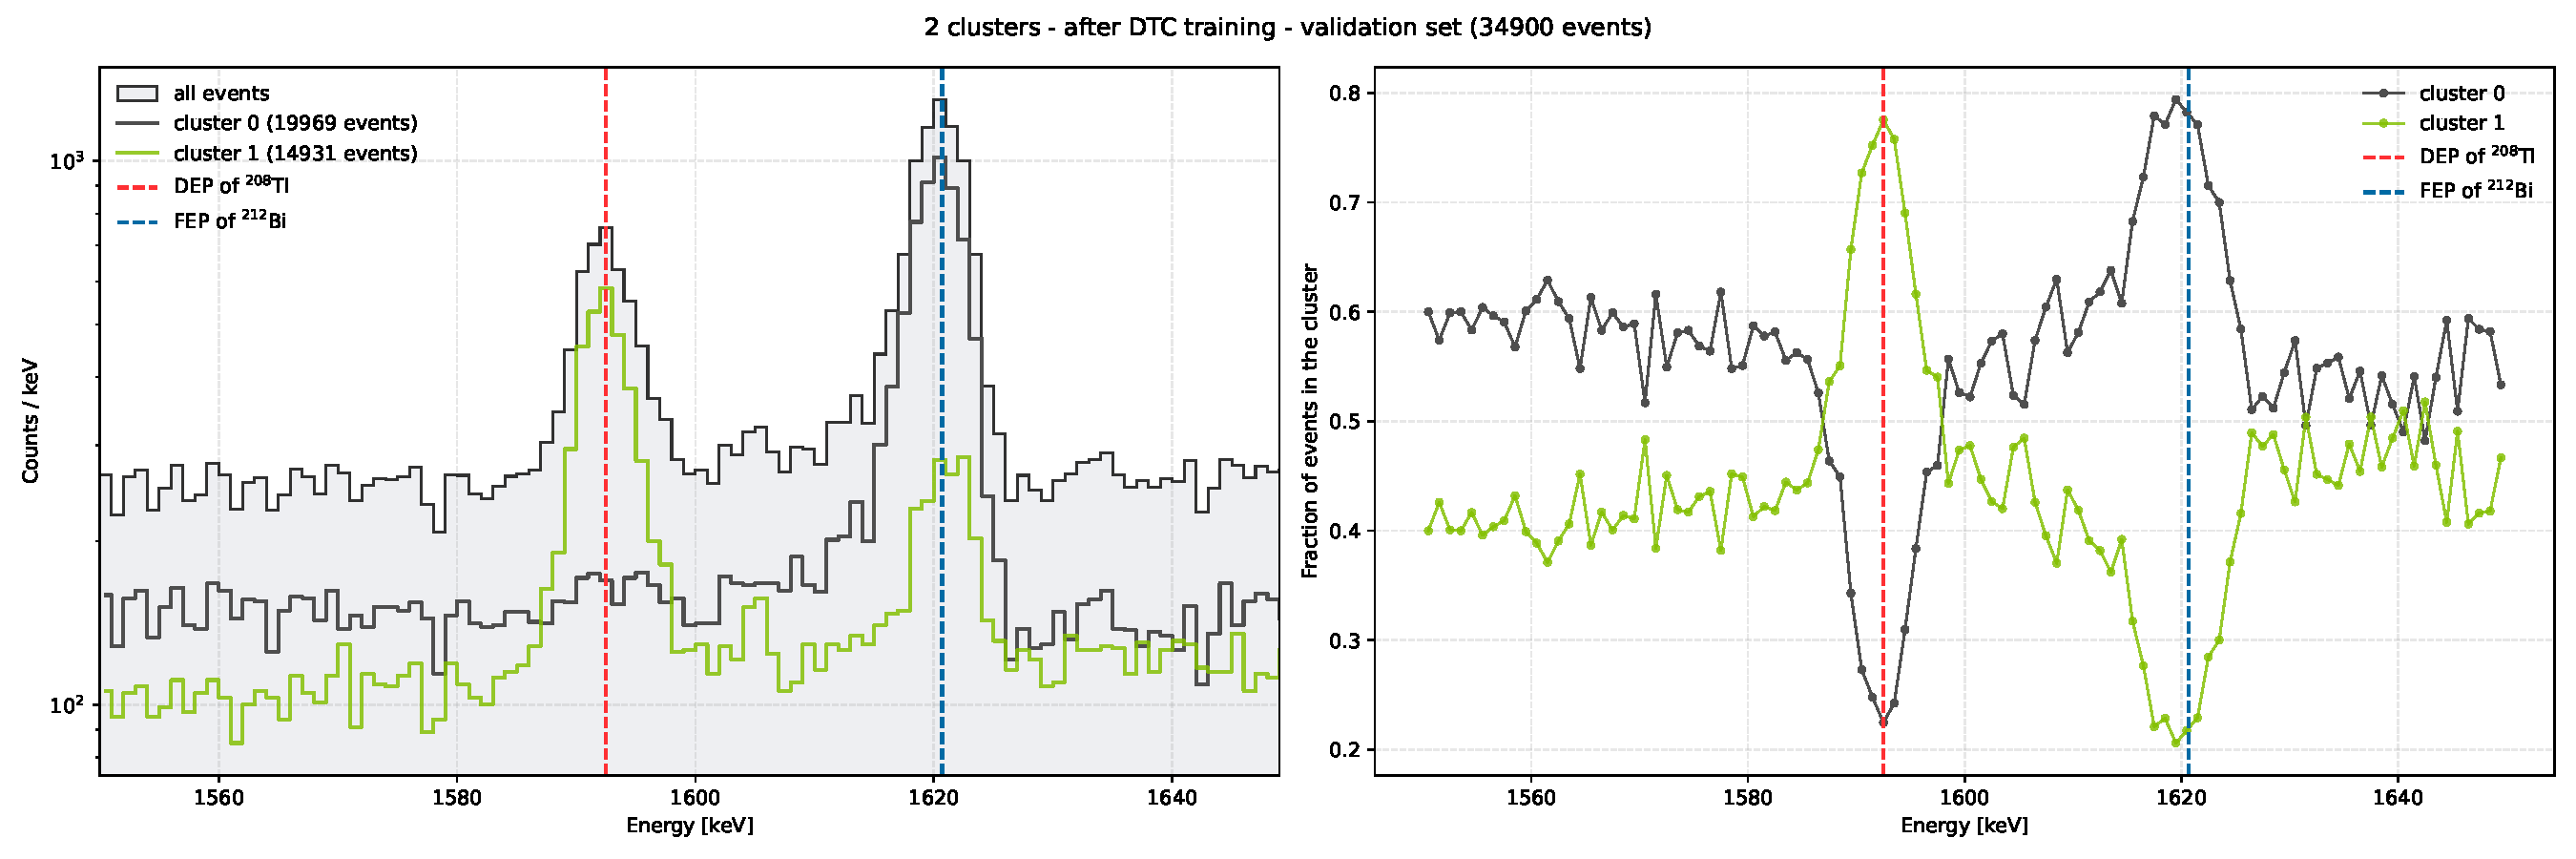
\includegraphics[width=\textwidth,height=0.27\textheight,keepaspectratio]{plots/DTC/euclidean/eucl_2cl_energy_val.pdf}\\[2pt]
    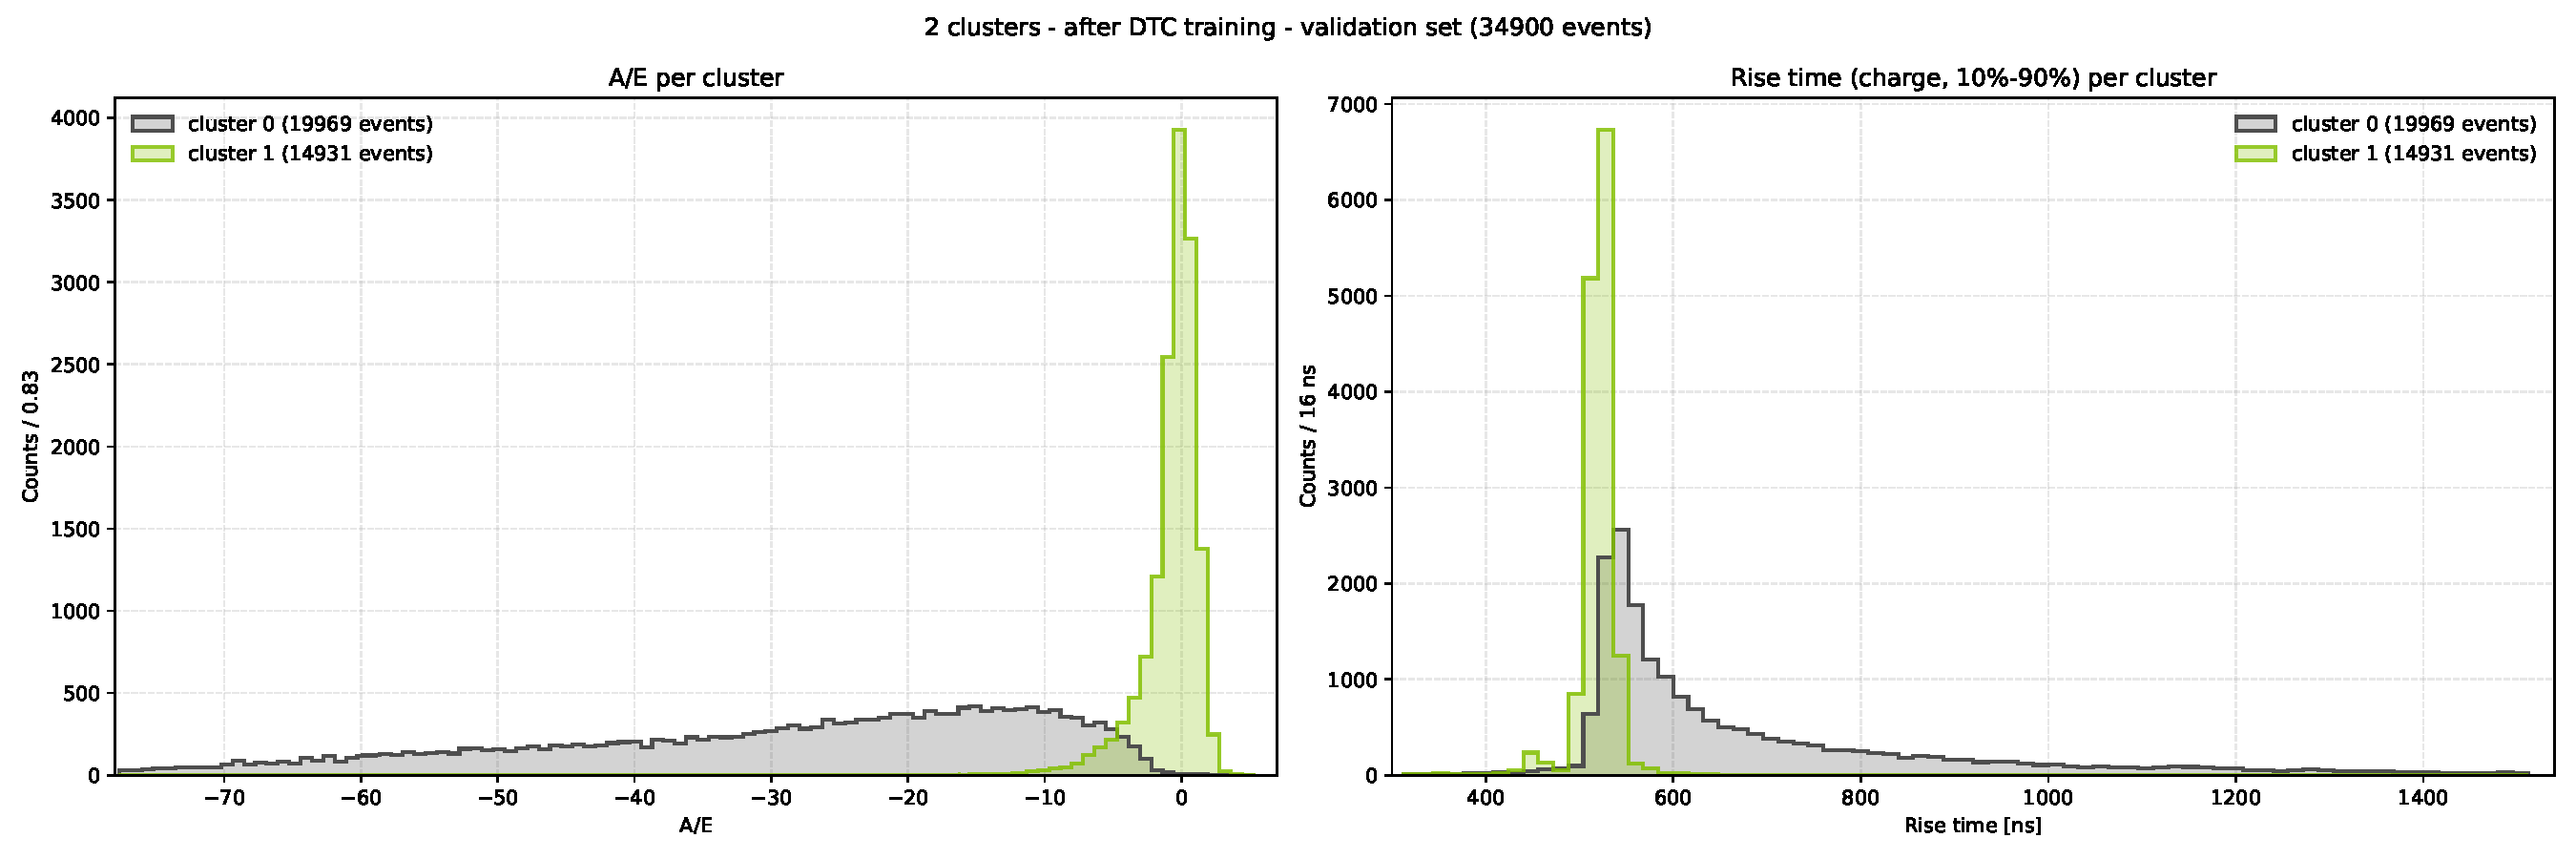
\includegraphics[width=\textwidth,height=0.27\textheight,keepaspectratio]{plots/DTC/euclidean/eucl_2cl_AoE_risetime_val_linear.pdf}\\[2pt]
    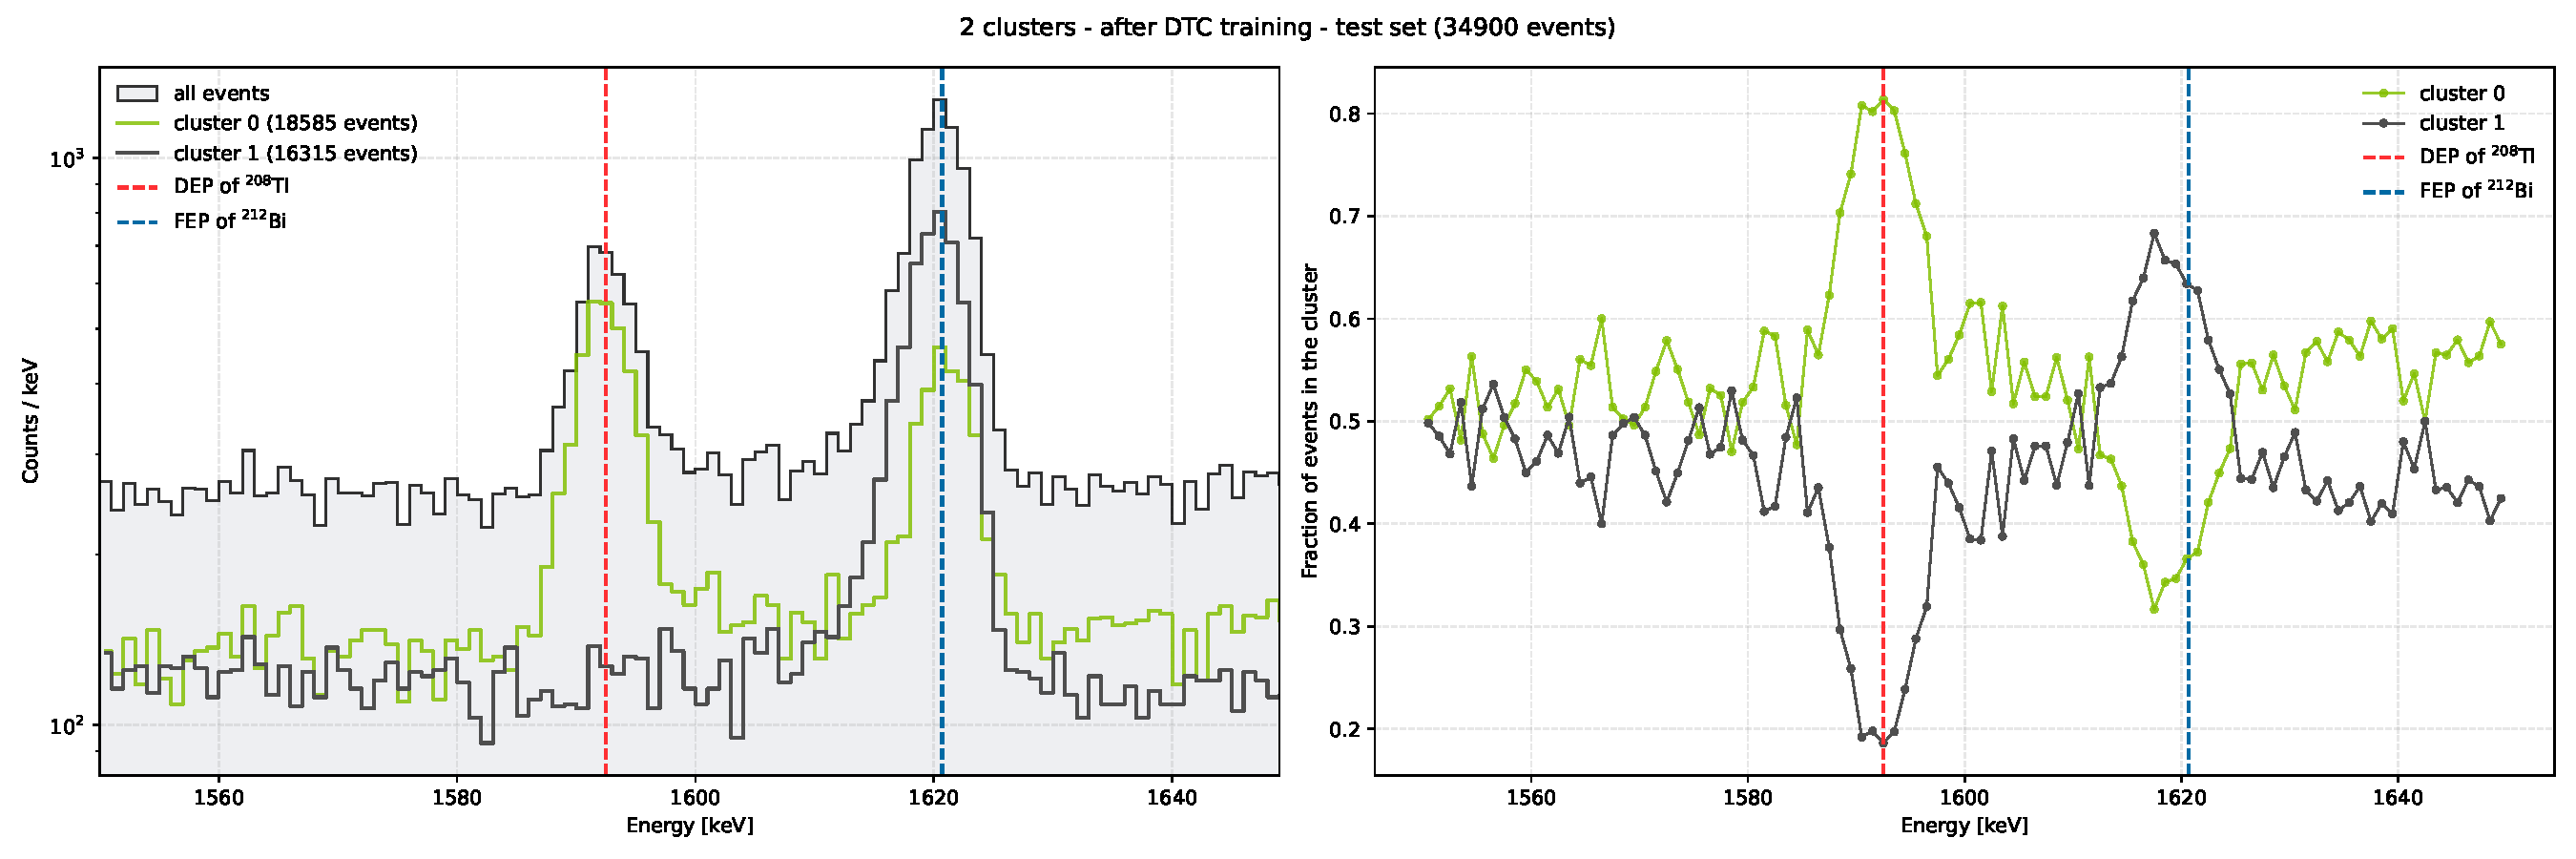
\includegraphics[width=\textwidth,height=0.27\textheight,keepaspectratio]{plots/DTC/euclidean/eucl_2cl_energy_test.pdf}\\[2pt]
    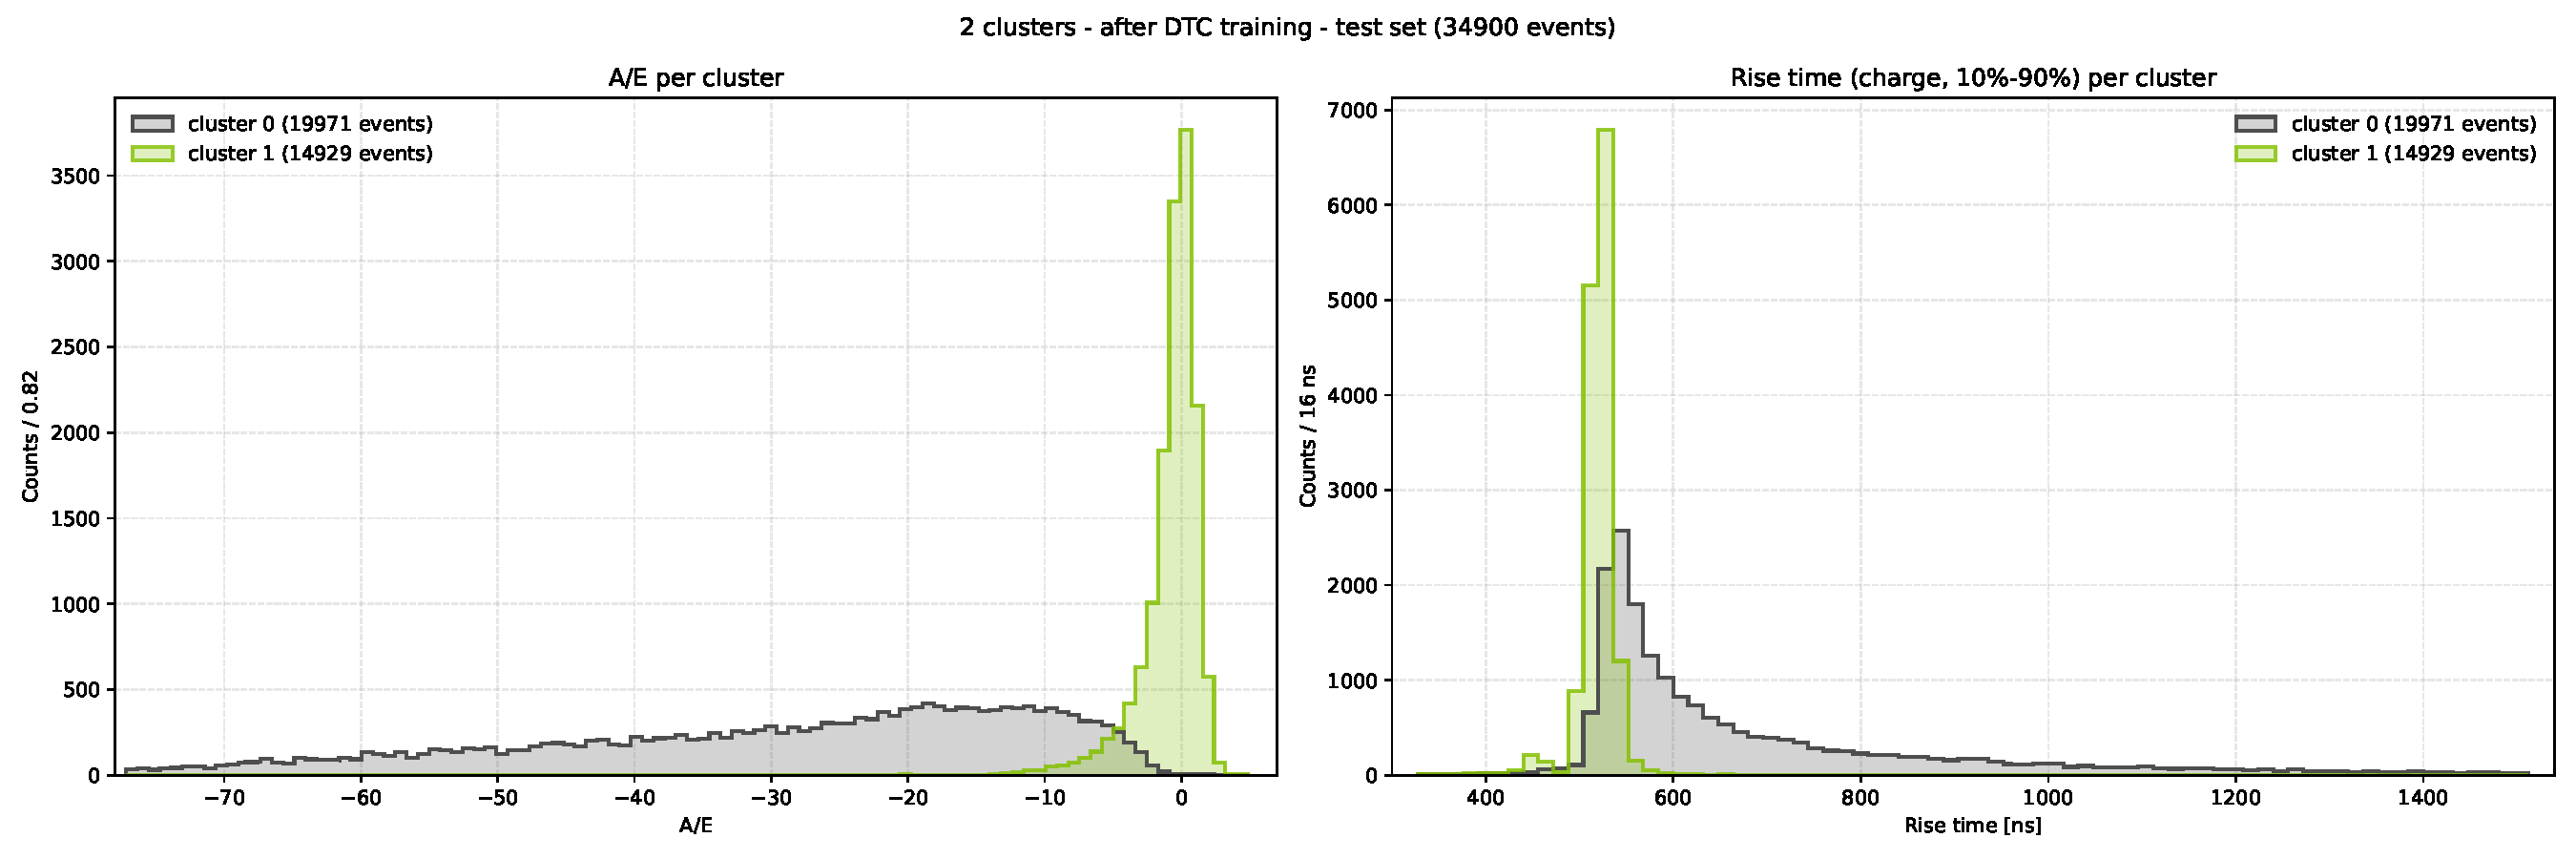
\includegraphics[width=\textwidth,height=0.27\textheight,keepaspectratio]{plots/DTC/euclidean/eucl_2cl_AoE_risetime_test_linear.pdf}
    \caption{Clustering results with the \ac{EUC} metric on the validation set (first and second rows) and on the test set (third and fourth rows): energy spectrum of each cluster and fraction of events assigned to each cluster as a function of energy (first and third rows), and \ac{AE} and rise time distributions of the two clusters (second and fourth rows).}
    \label{fig:euclidean-aoe}
    \label{fig:euclidean-aoe-train}
    \label{fig:euclidean-aoe-valid}
    \label{fig:euclidean-aoe-test}
\end{figure}

\begin{figure}[H]
    \centering
    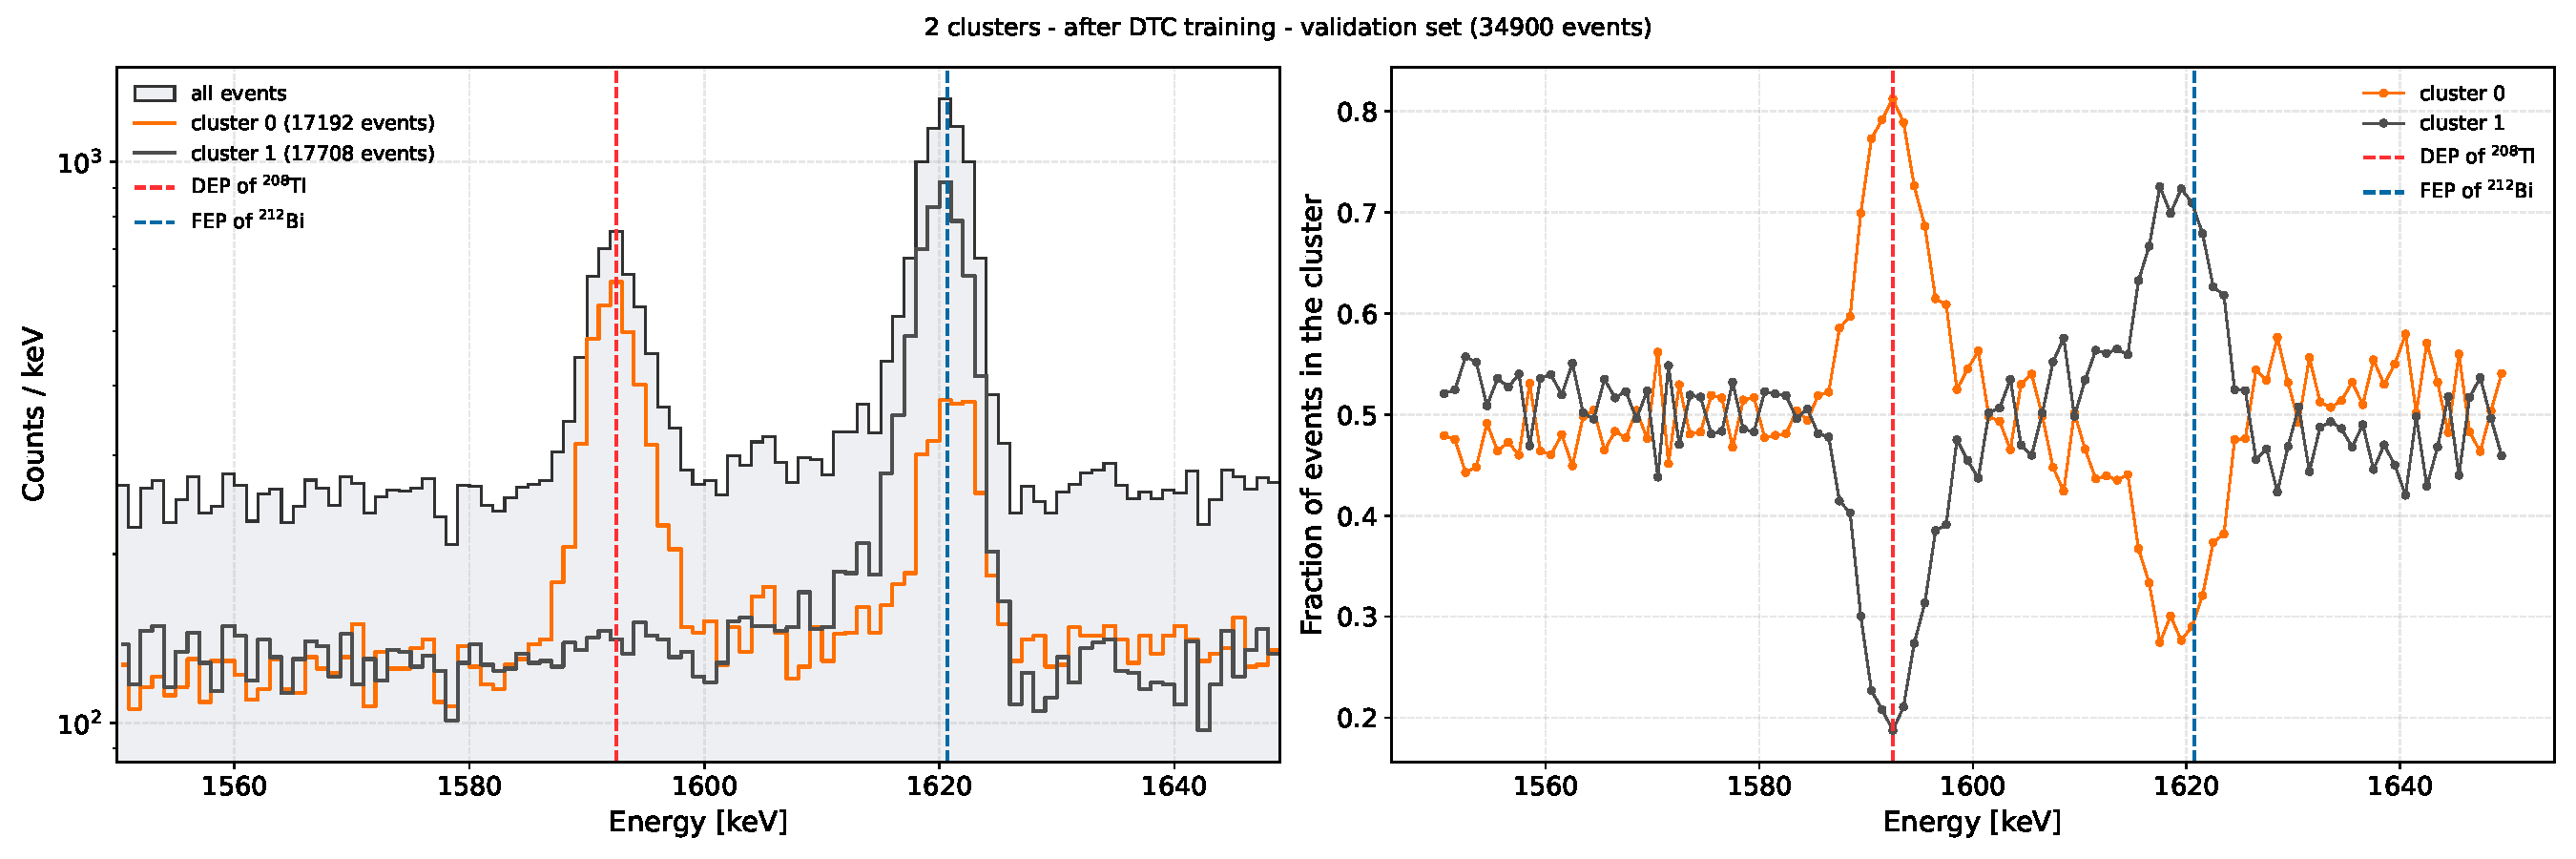
\includegraphics[width=\textwidth,height=0.27\textheight,keepaspectratio]{plots/DTC/cid/cid_2cl_energy_val.pdf}\\[2pt]
    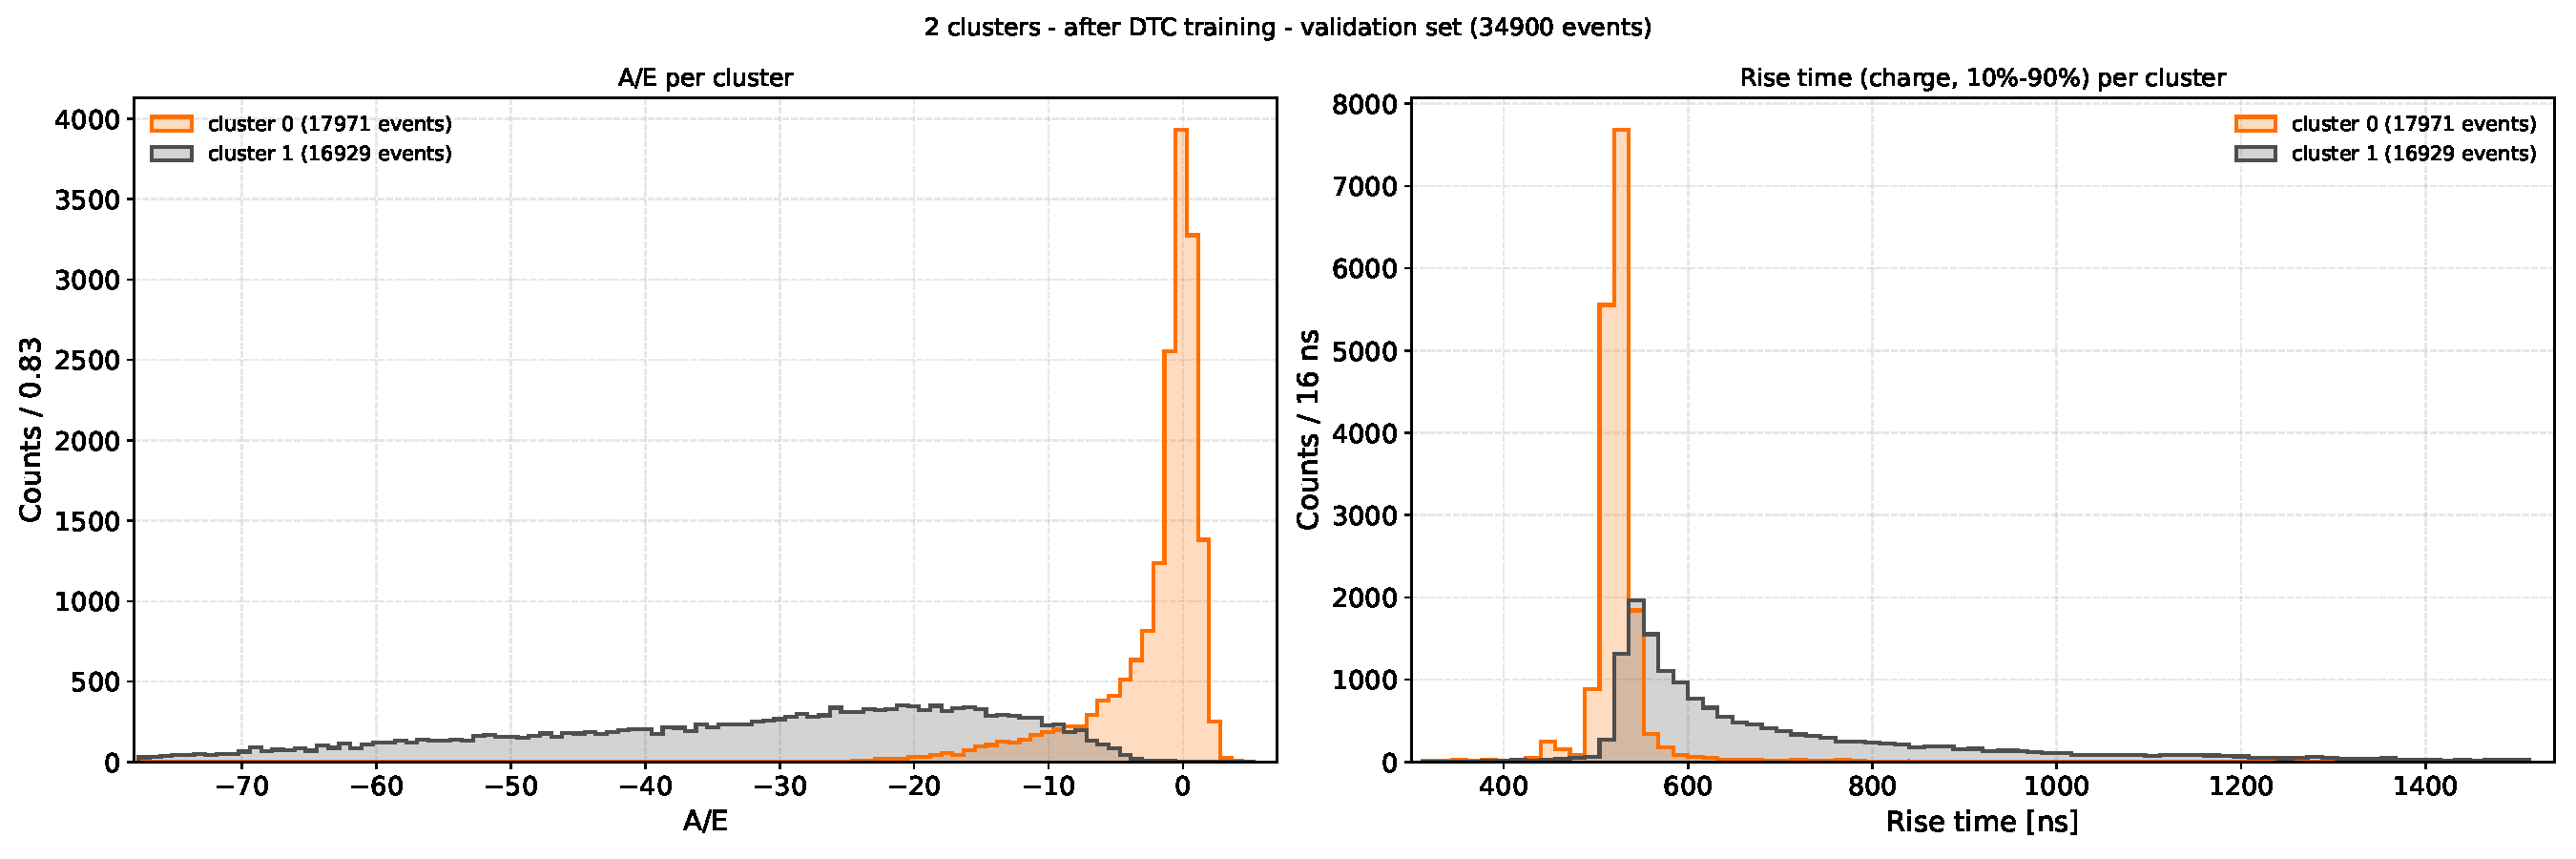
\includegraphics[width=\textwidth,height=0.27\textheight,keepaspectratio]{plots/DTC/cid/cid_2cl_AoE_risetime_val_linear.pdf}\\[2pt]
    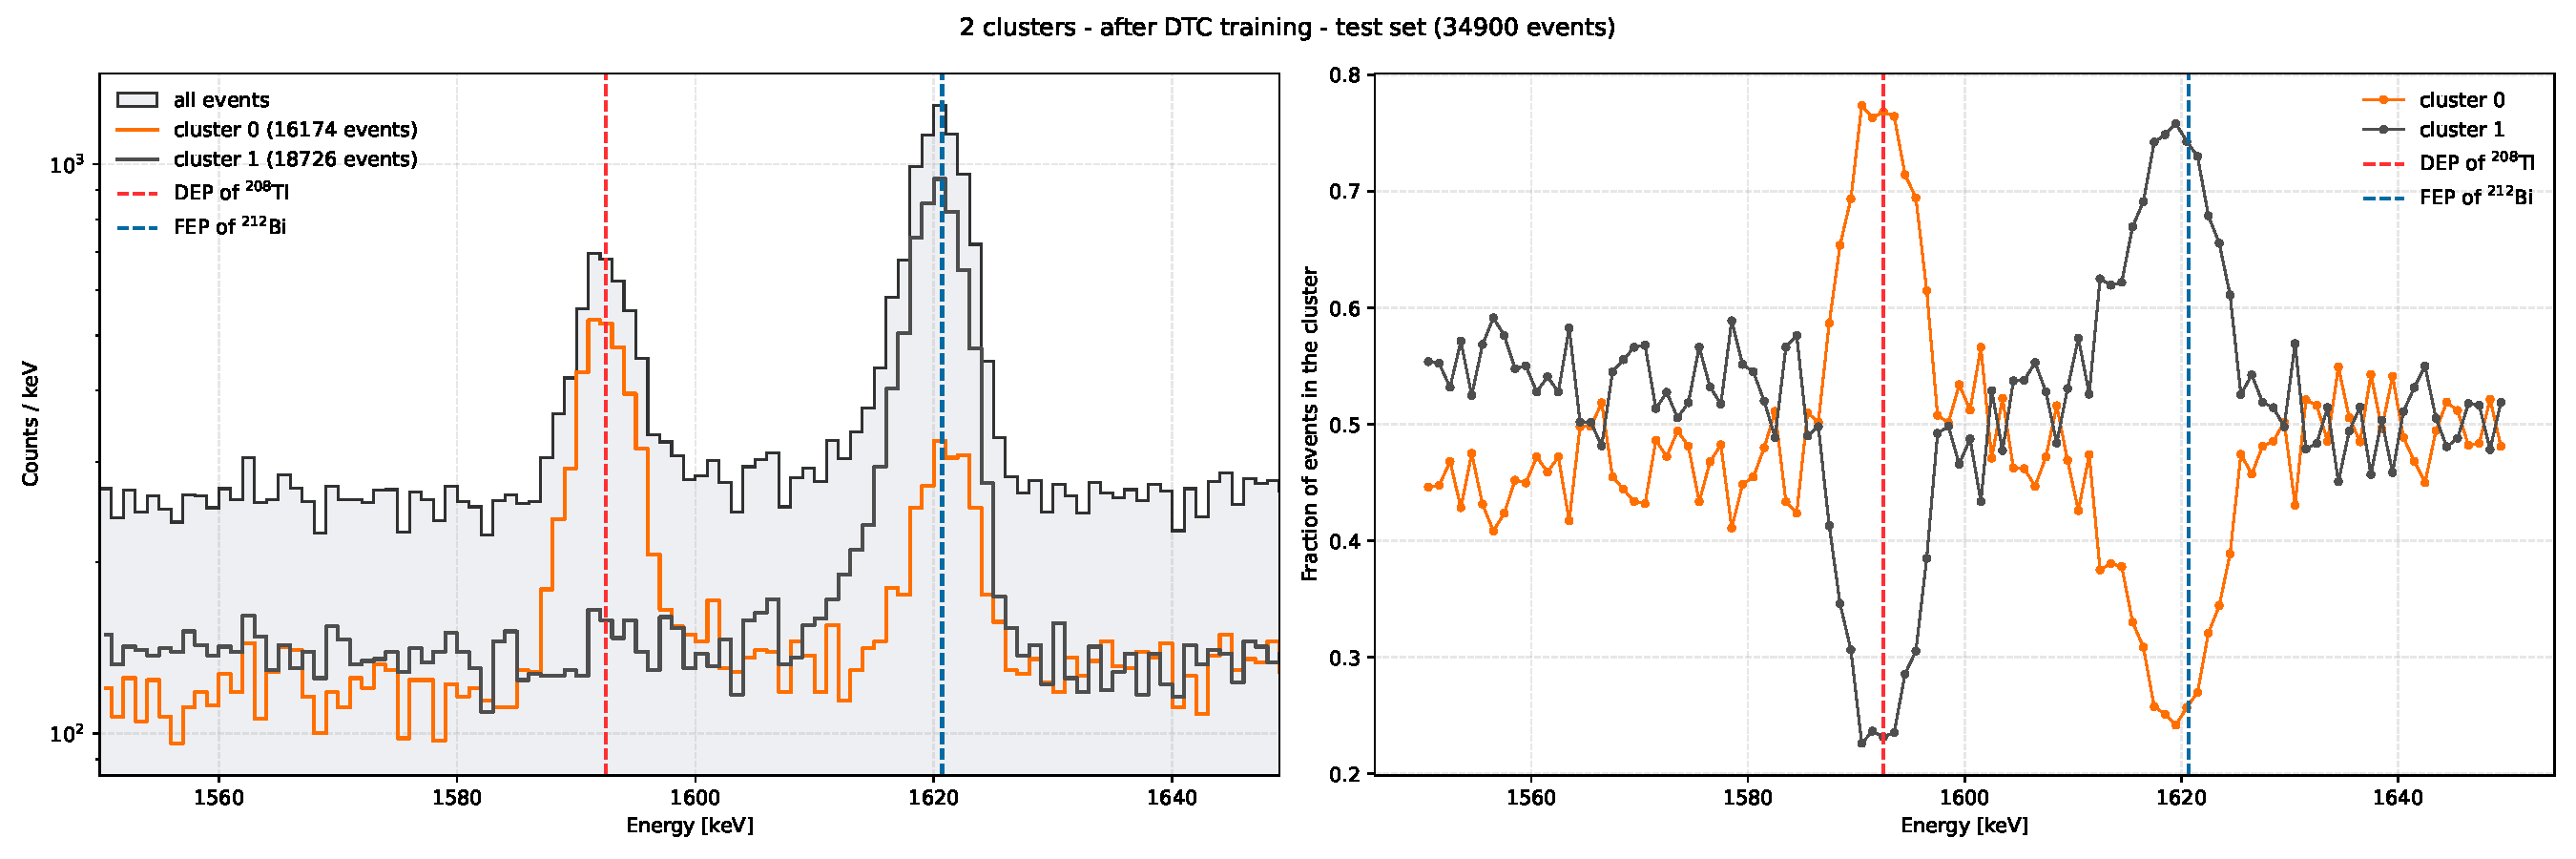
\includegraphics[width=\textwidth,height=0.27\textheight,keepaspectratio]{plots/DTC/cid/cid_2cl_energy_test.pdf}\\[2pt]
    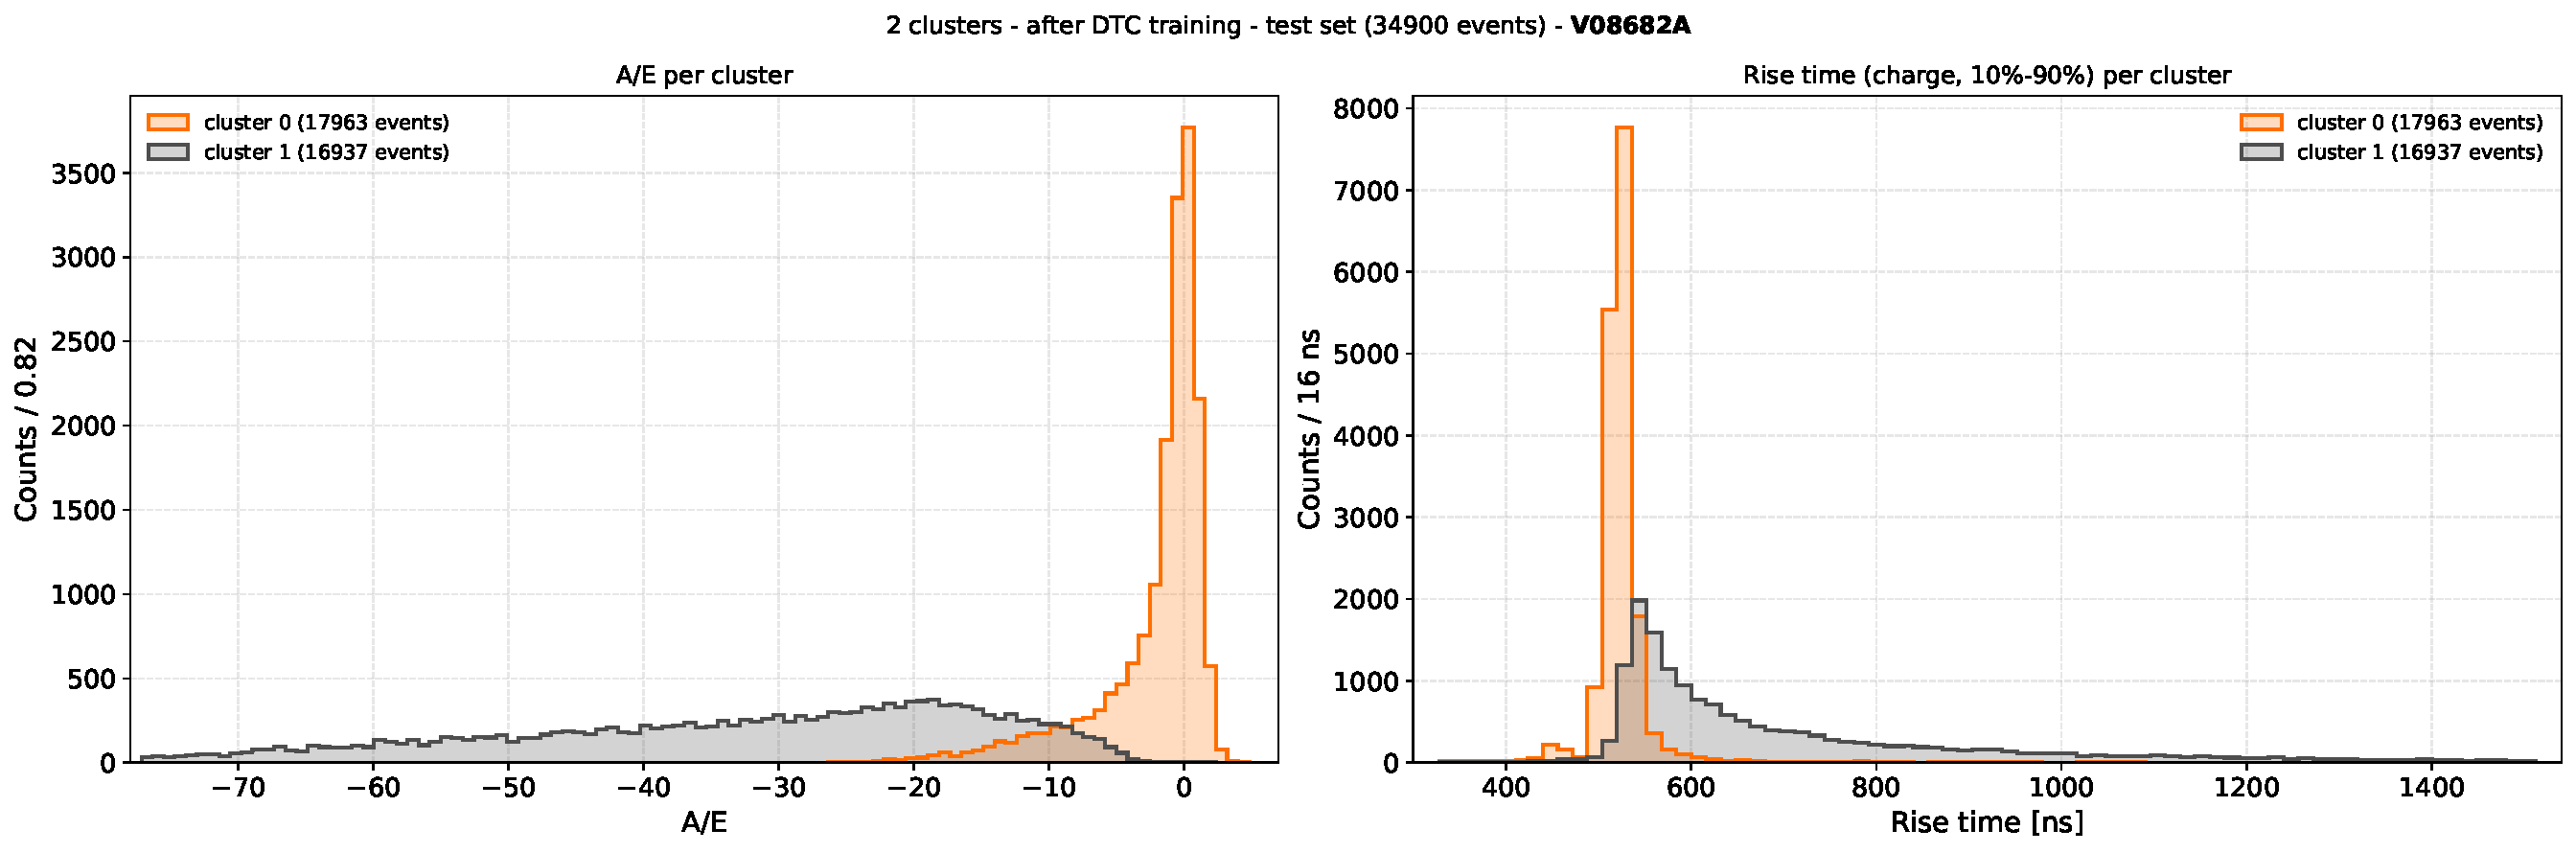
\includegraphics[width=\textwidth,height=0.27\textheight,keepaspectratio]{plots/DTC/cid/cid_2cl_AoE_risetime_test_linear.pdf}
    \caption{Clustering results with the \ac{CID} metric on the validation set (first and second rows) and on the test set (third and fourth rows): energy spectrum of each cluster and fraction of events assigned to each cluster as a function of energy (first and third rows), and \ac{AE} and rise time distributions of the two clusters (second and fourth rows).}
    \label{fig:cid-aoe}
    \label{fig:cid-aoe-train}
    \label{fig:cid-aoe-valid}
    \label{fig:cid-aoe-test}
\end{figure}

\section{V08682B}
 Figs.~\ref{fig:acf-training-V08682B}-\ref{fig:cid-training-V08682B} show the reconstruction of a fixed validation waveform at different epochs together with the evolution of the training and validation losses, while Figs.~\ref{fig:acf-aoe-V08682B}-\ref{fig:cid-aoe-V08682B} show the clustering results and the \ac{AE} and rise time distributions of the two clusters for the validation and test sets.

 %==================================================
% Reconstruction and losses
%==================================================

\begin{figure}[H]
    \centering
    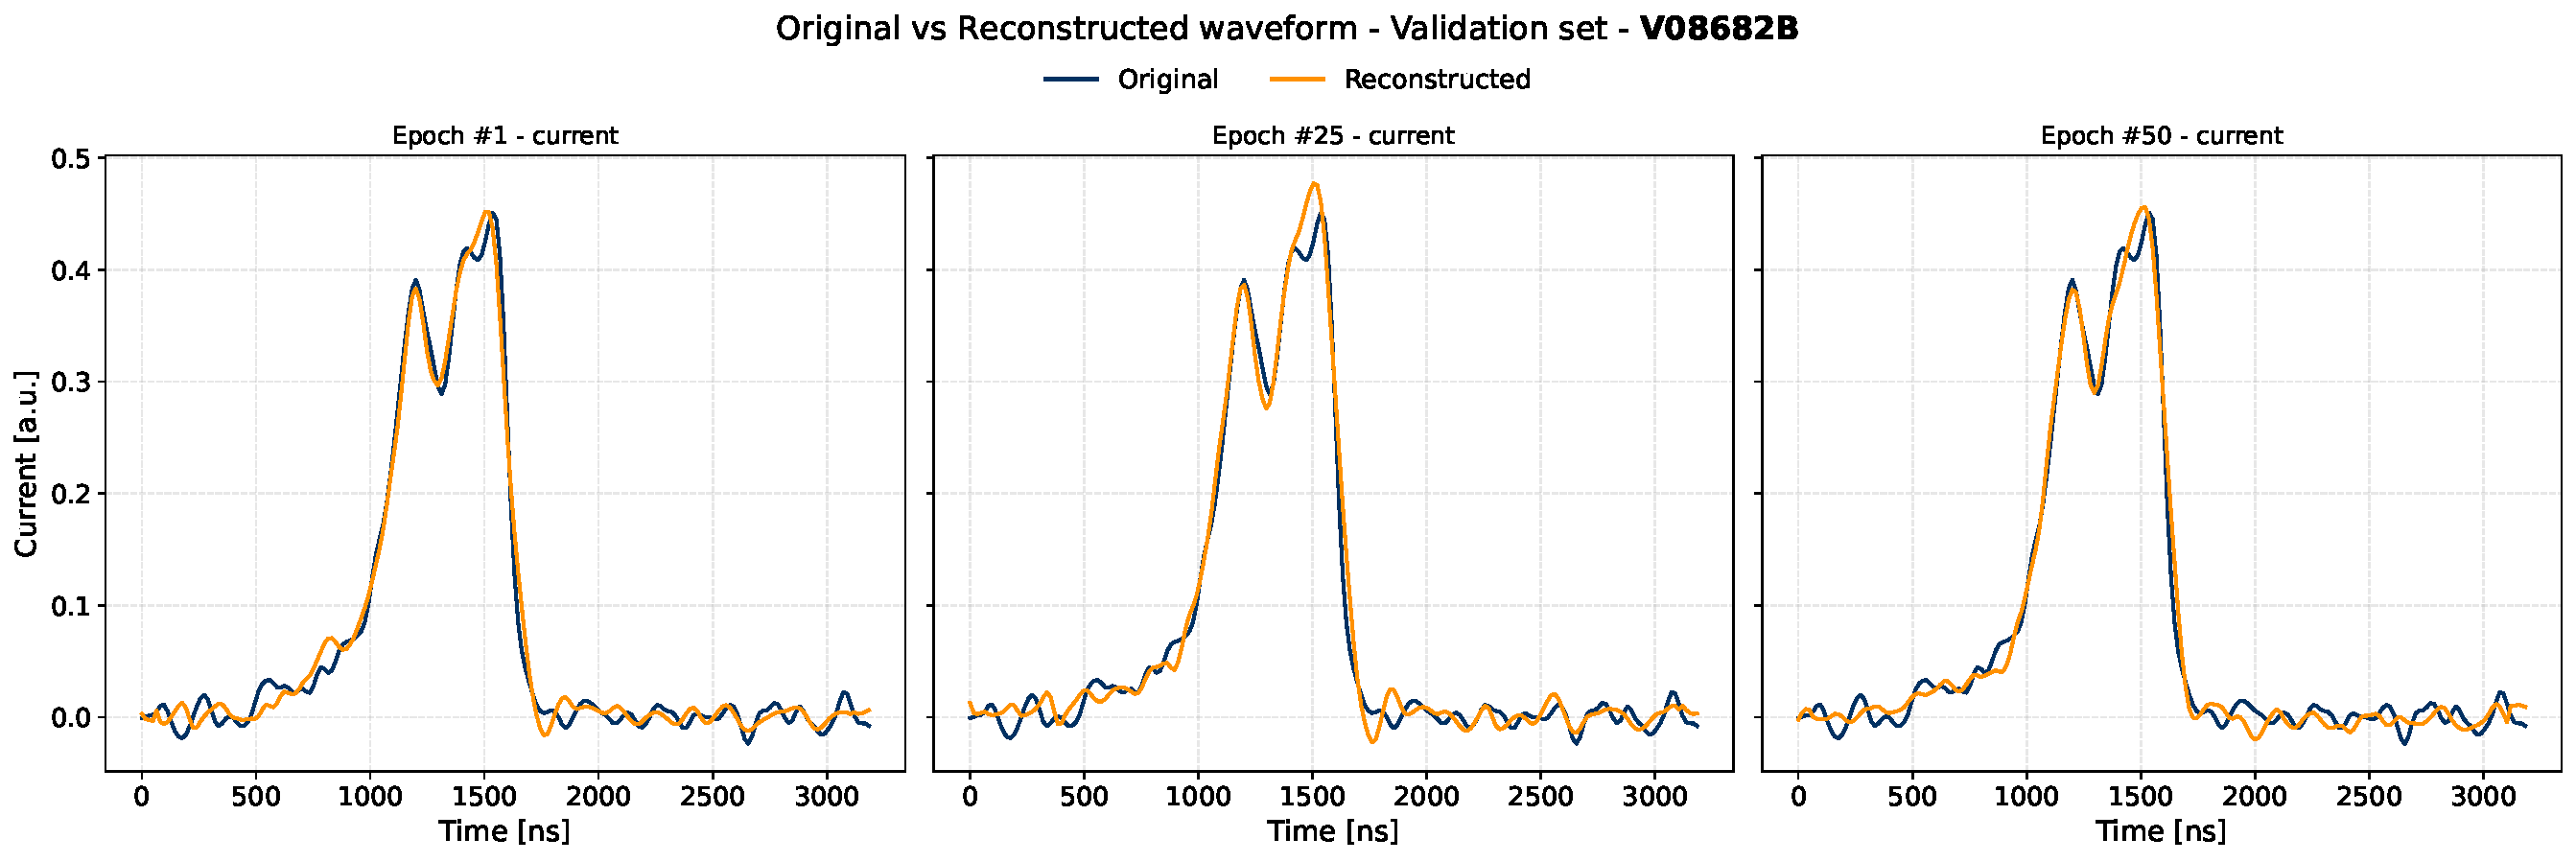
\includegraphics[width=\textwidth,height=0.36\textheight,keepaspectratio]{plots/V08682B/DTC/acf_2cl_training_reconstruction.pdf}\\[4pt]
    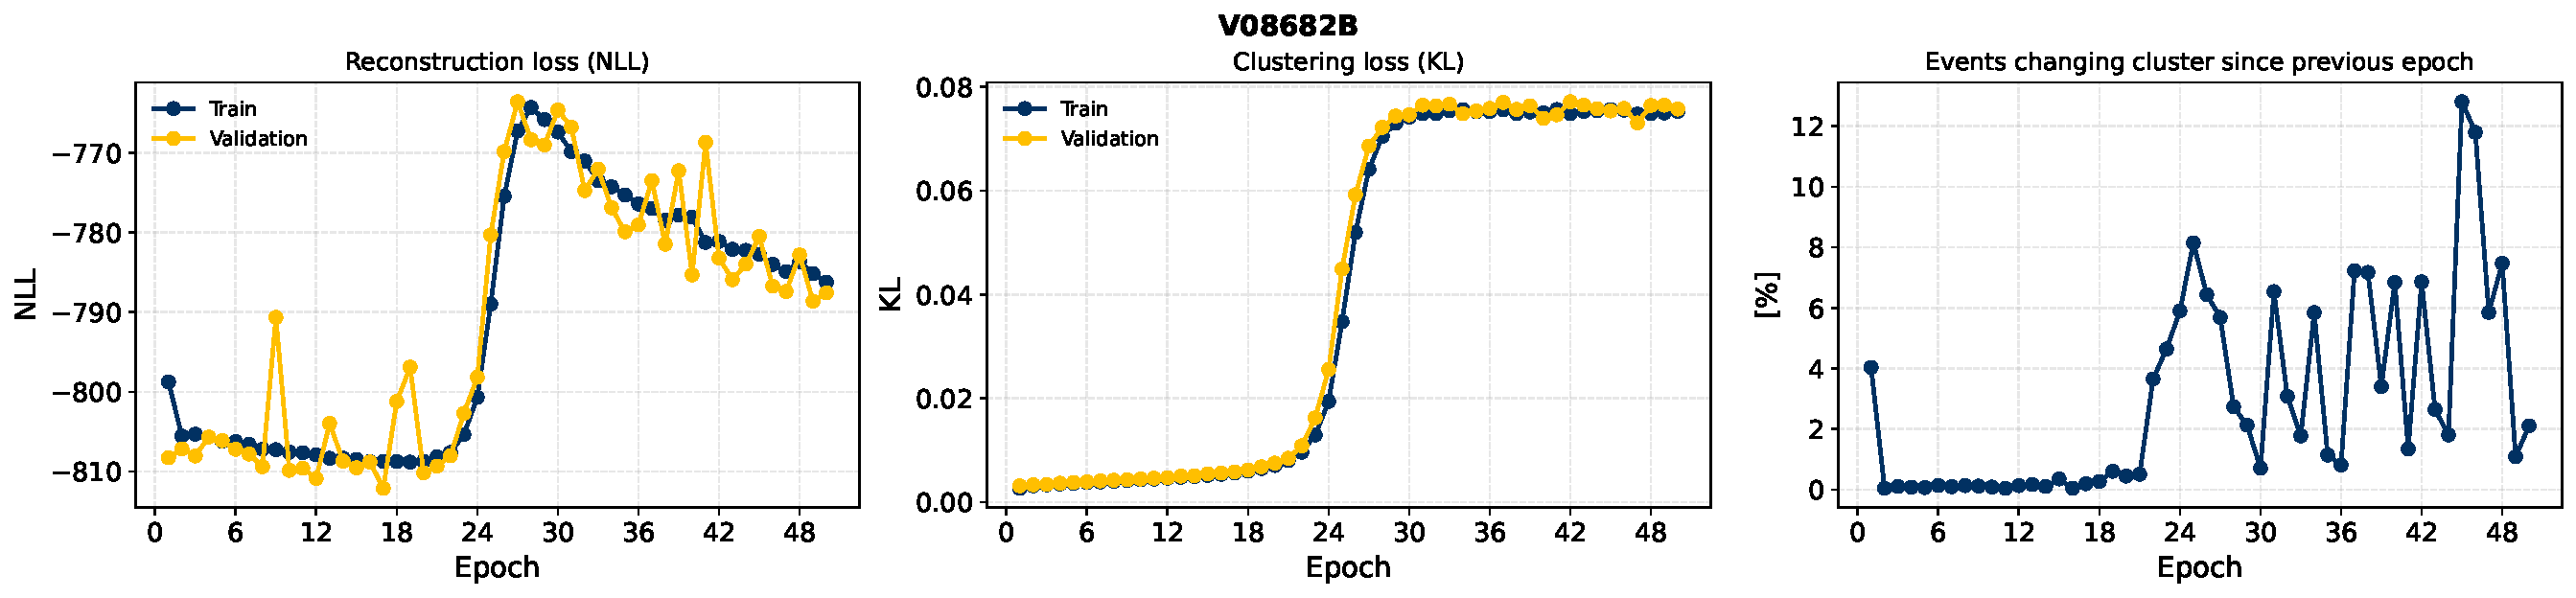
\includegraphics[width=\textwidth,height=0.36\textheight,keepaspectratio]{plots/V08682B/DTC/acf_2cl_training_history.pdf}
    \caption{Reconstructed waveforms through epochs (top), losses and fraction of events changing cluster per epoch (bottom) with the \ac{ACF} metric - V08682B.}
    \label{fig:acf-training-V08682B}
    \label{fig:acf-reconstruction-V08682B}
    \label{fig:acf-losses-V08682B}
\end{figure}

\begin{figure}[H]
    \centering
    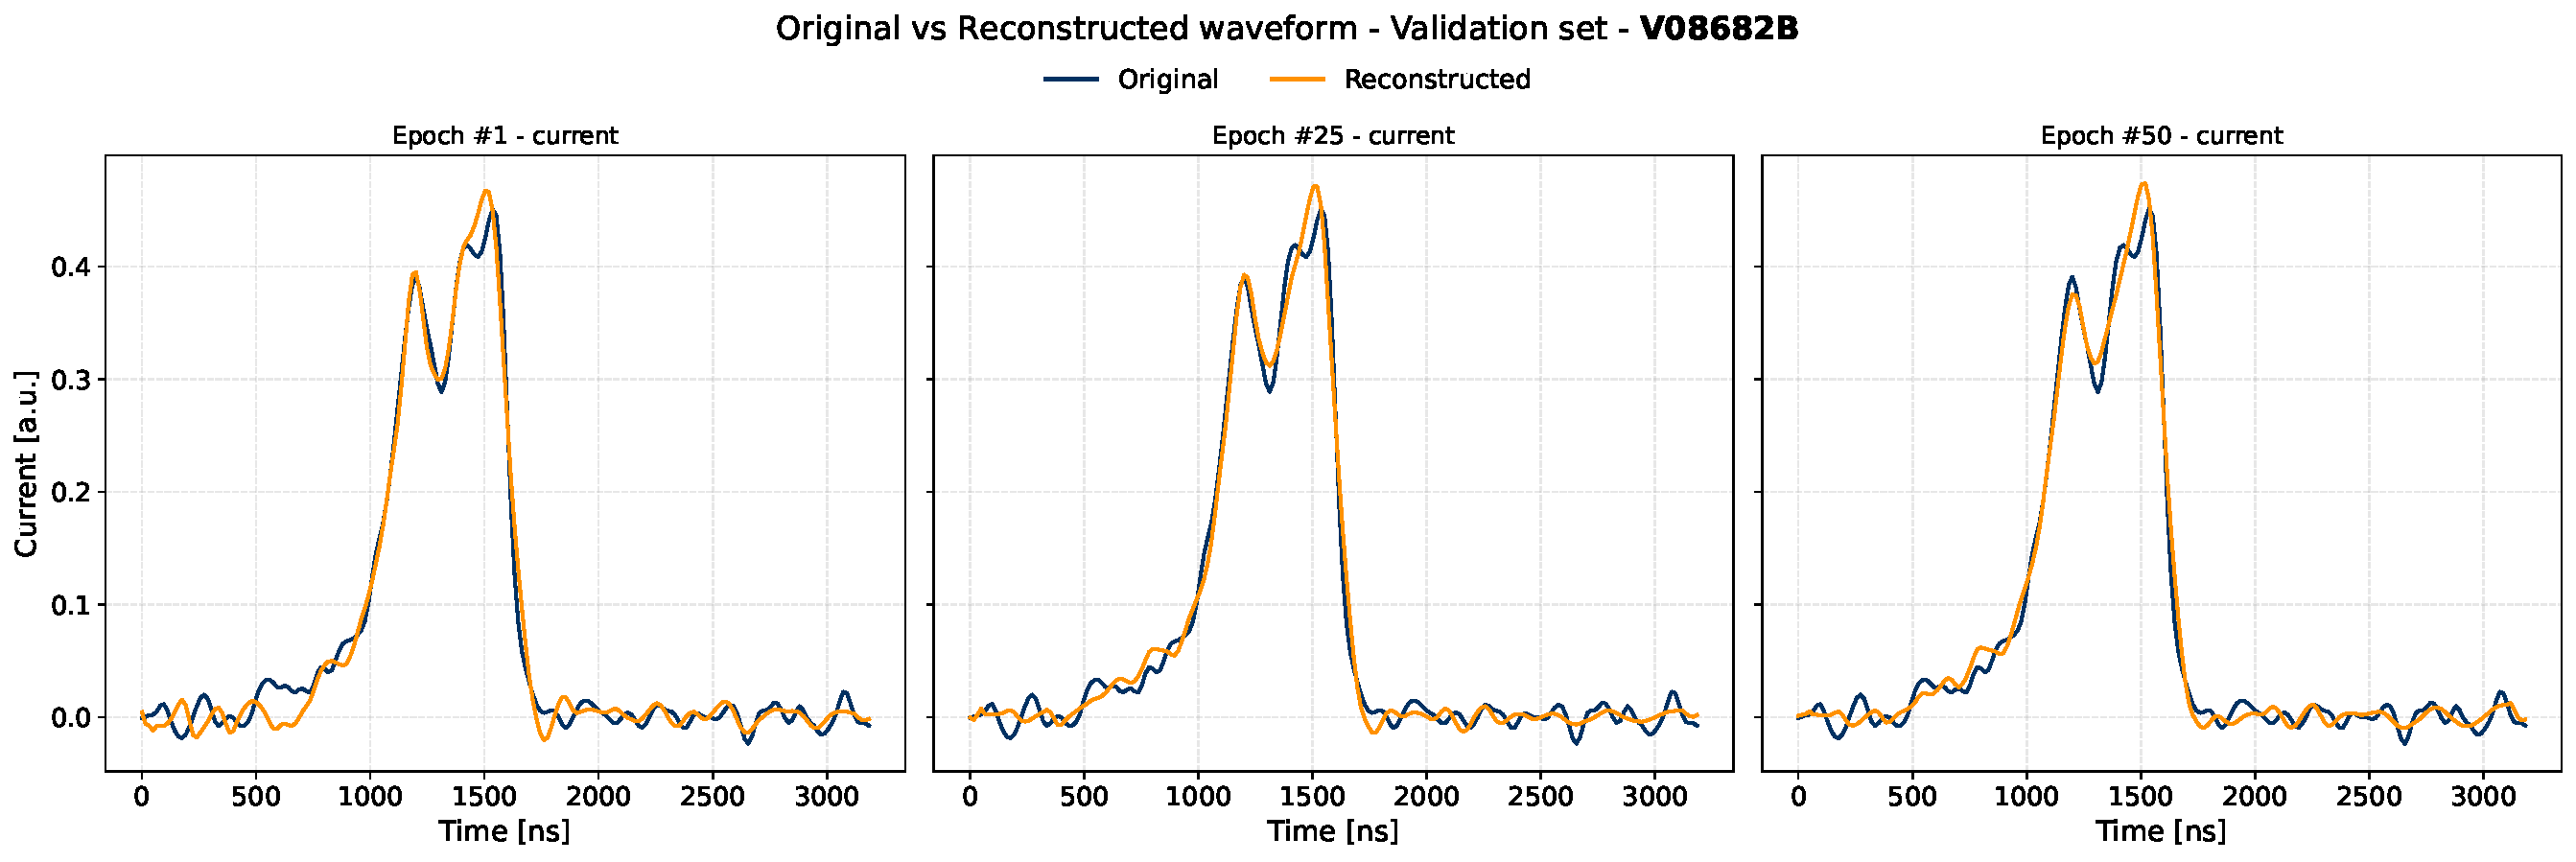
\includegraphics[width=\textwidth,height=0.36\textheight,keepaspectratio]{plots/V08682B/DTC/eucl_2cl_training_reconstruction.pdf}\\[4pt]
    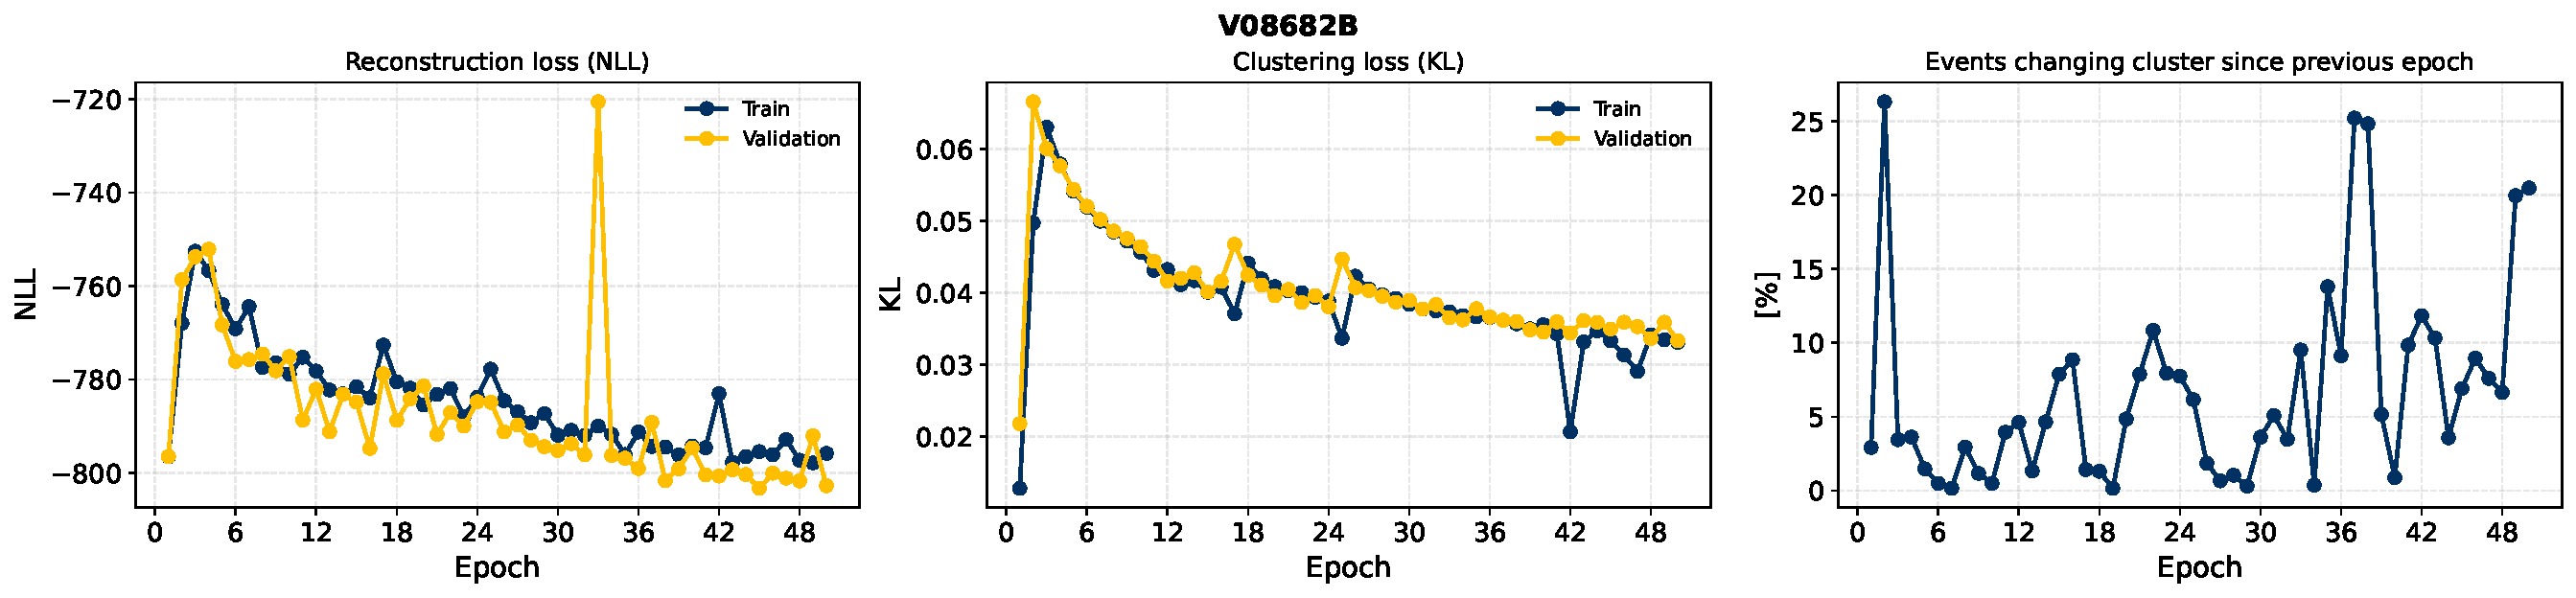
\includegraphics[width=\textwidth,height=0.36\textheight,keepaspectratio]{plots/V08682B/DTC/eucl_2cl_training_history.pdf}
    \caption{Reconstructed waveforms through epochs (top), losses and fraction of events changing cluster per epoch (bottom) with the \ac{EUC} metric - V08682B.}
    \label{fig:euclidean-training-V08682B}
    \label{fig:euclidean-reconstruction-V08682B}
    \label{fig:euclidean-losses-V08682B}
\end{figure}

\begin{figure}[H]
    \centering
    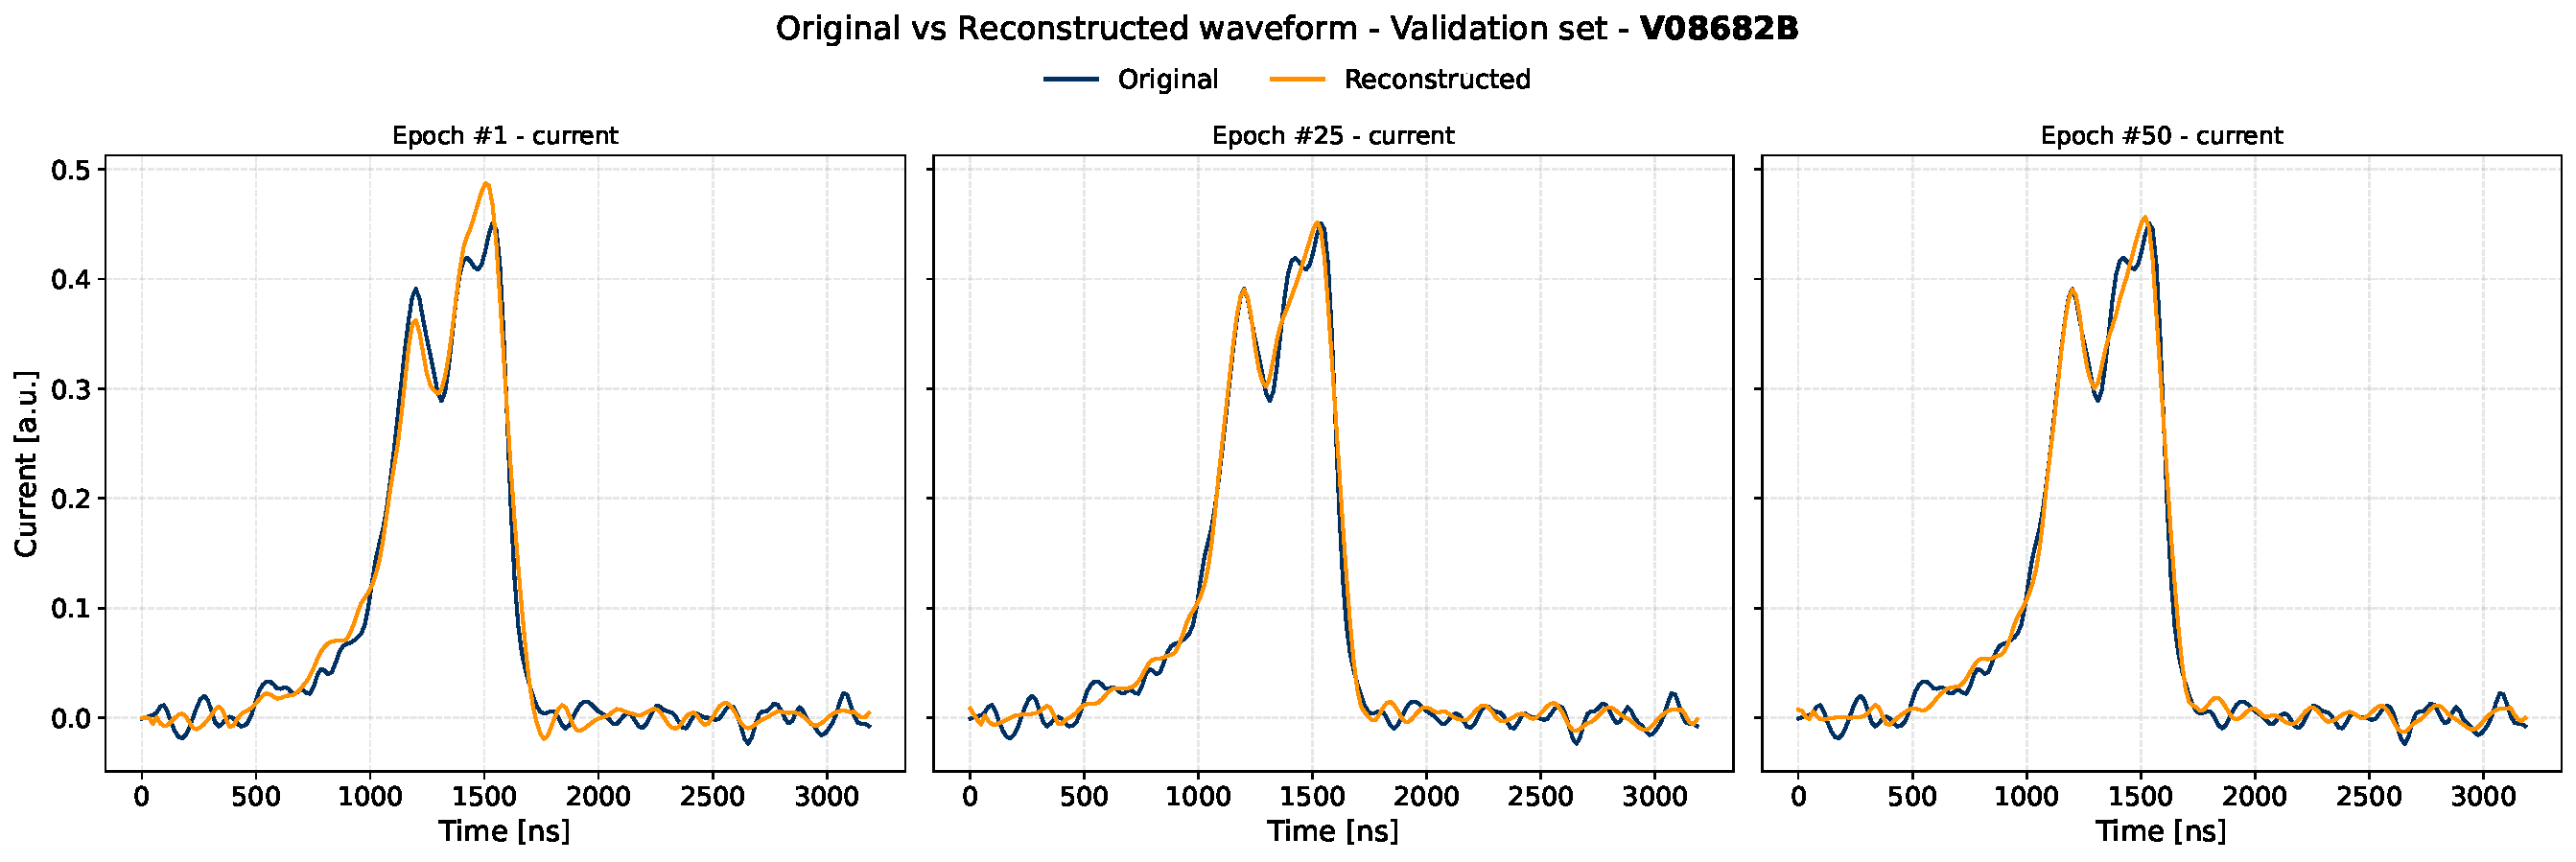
\includegraphics[width=\textwidth,height=0.36\textheight,keepaspectratio]{plots/V08682B/DTC/cid_2cl_training_reconstruction.pdf}\\[4pt]
    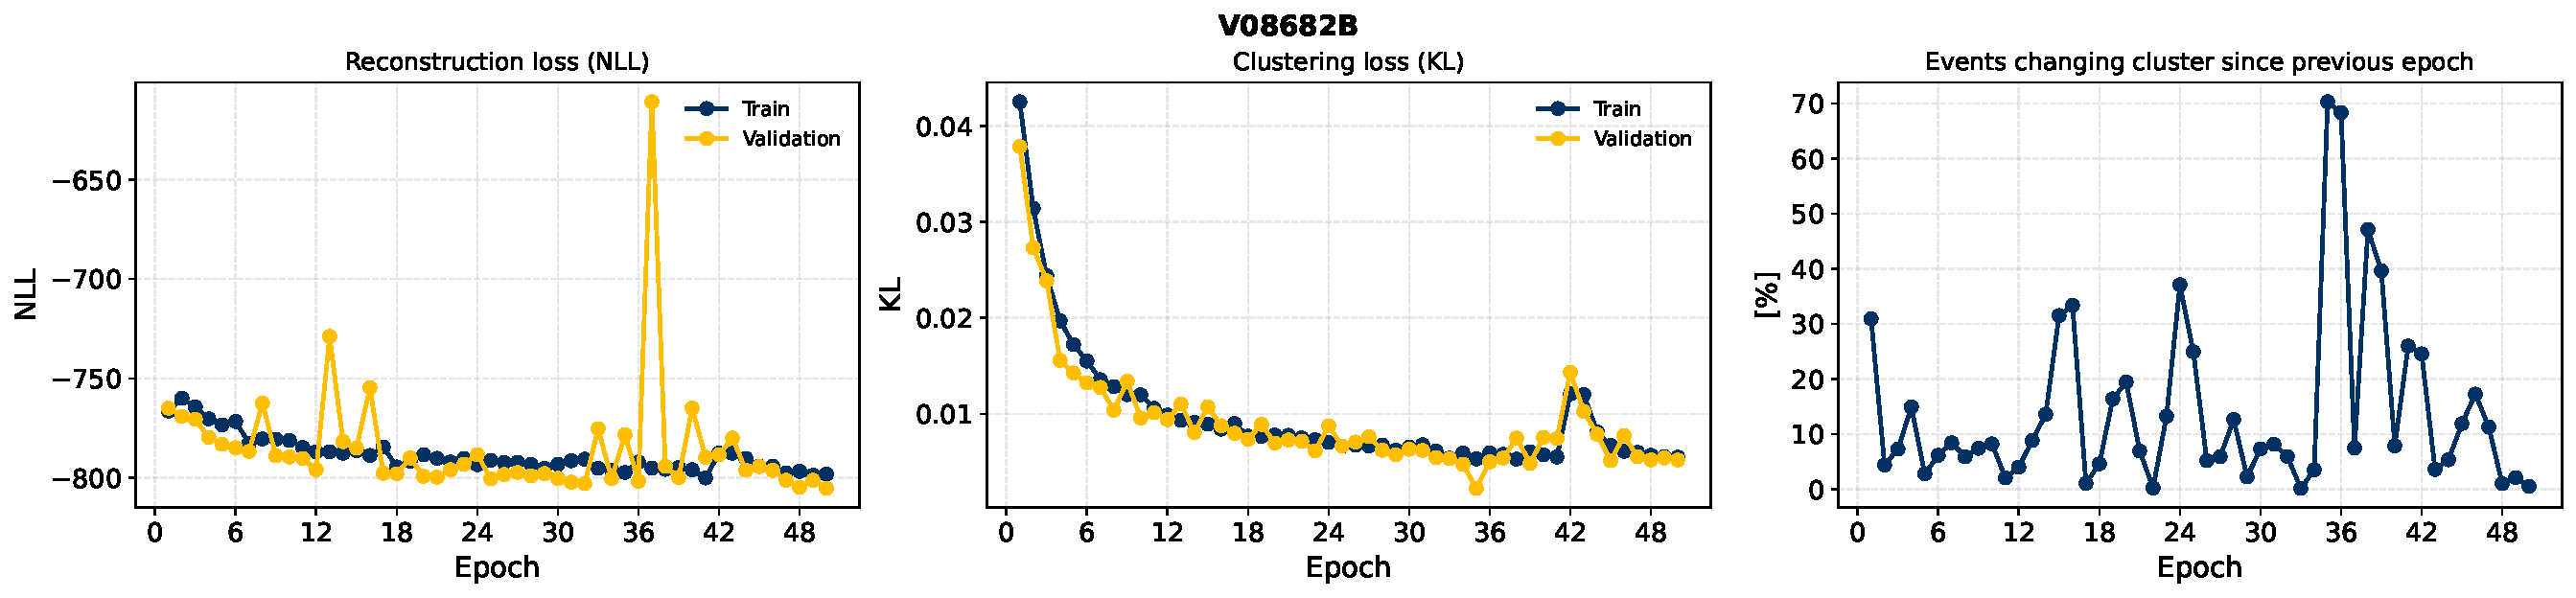
\includegraphics[width=\textwidth,height=0.36\textheight,keepaspectratio]{plots/V08682B/DTC/cid_2cl_training_history.pdf}
    \caption{Reconstructed waveforms through epochs (top), losses and fraction of events changing cluster per epoch (bottom) with the \ac{CID} metric - V08682B.}
    \label{fig:cid-training-V08682B}
    \label{fig:cid-reconstruction-V08682B}
    \label{fig:cid-losses-V08682B}
\end{figure}

%==================================================
% Validation and test sets
%==================================================

\begin{figure}[H]
    \centering
    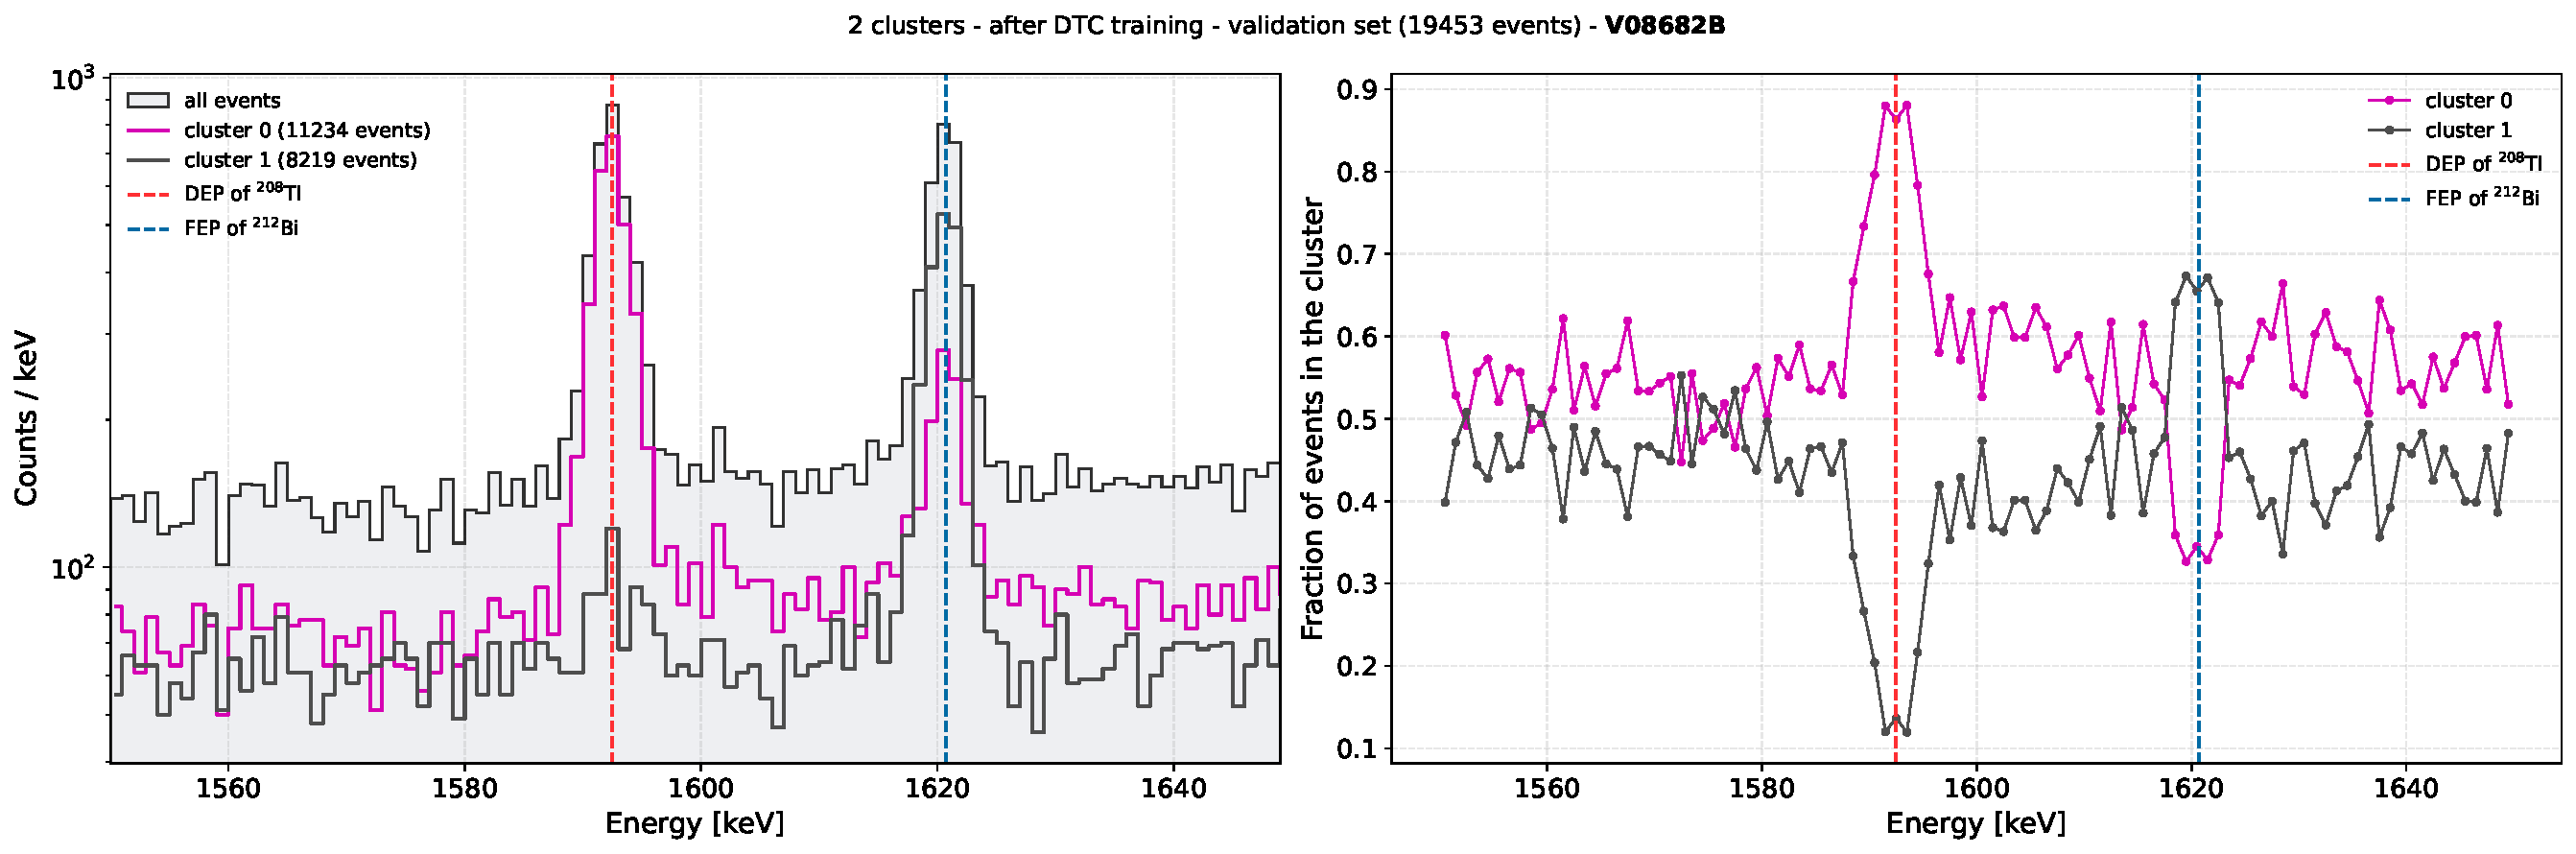
\includegraphics[width=\textwidth,height=0.27\textheight,keepaspectratio]{plots/V08682B/DTC/acf_2cl_energy_val.pdf}\\[2pt]
    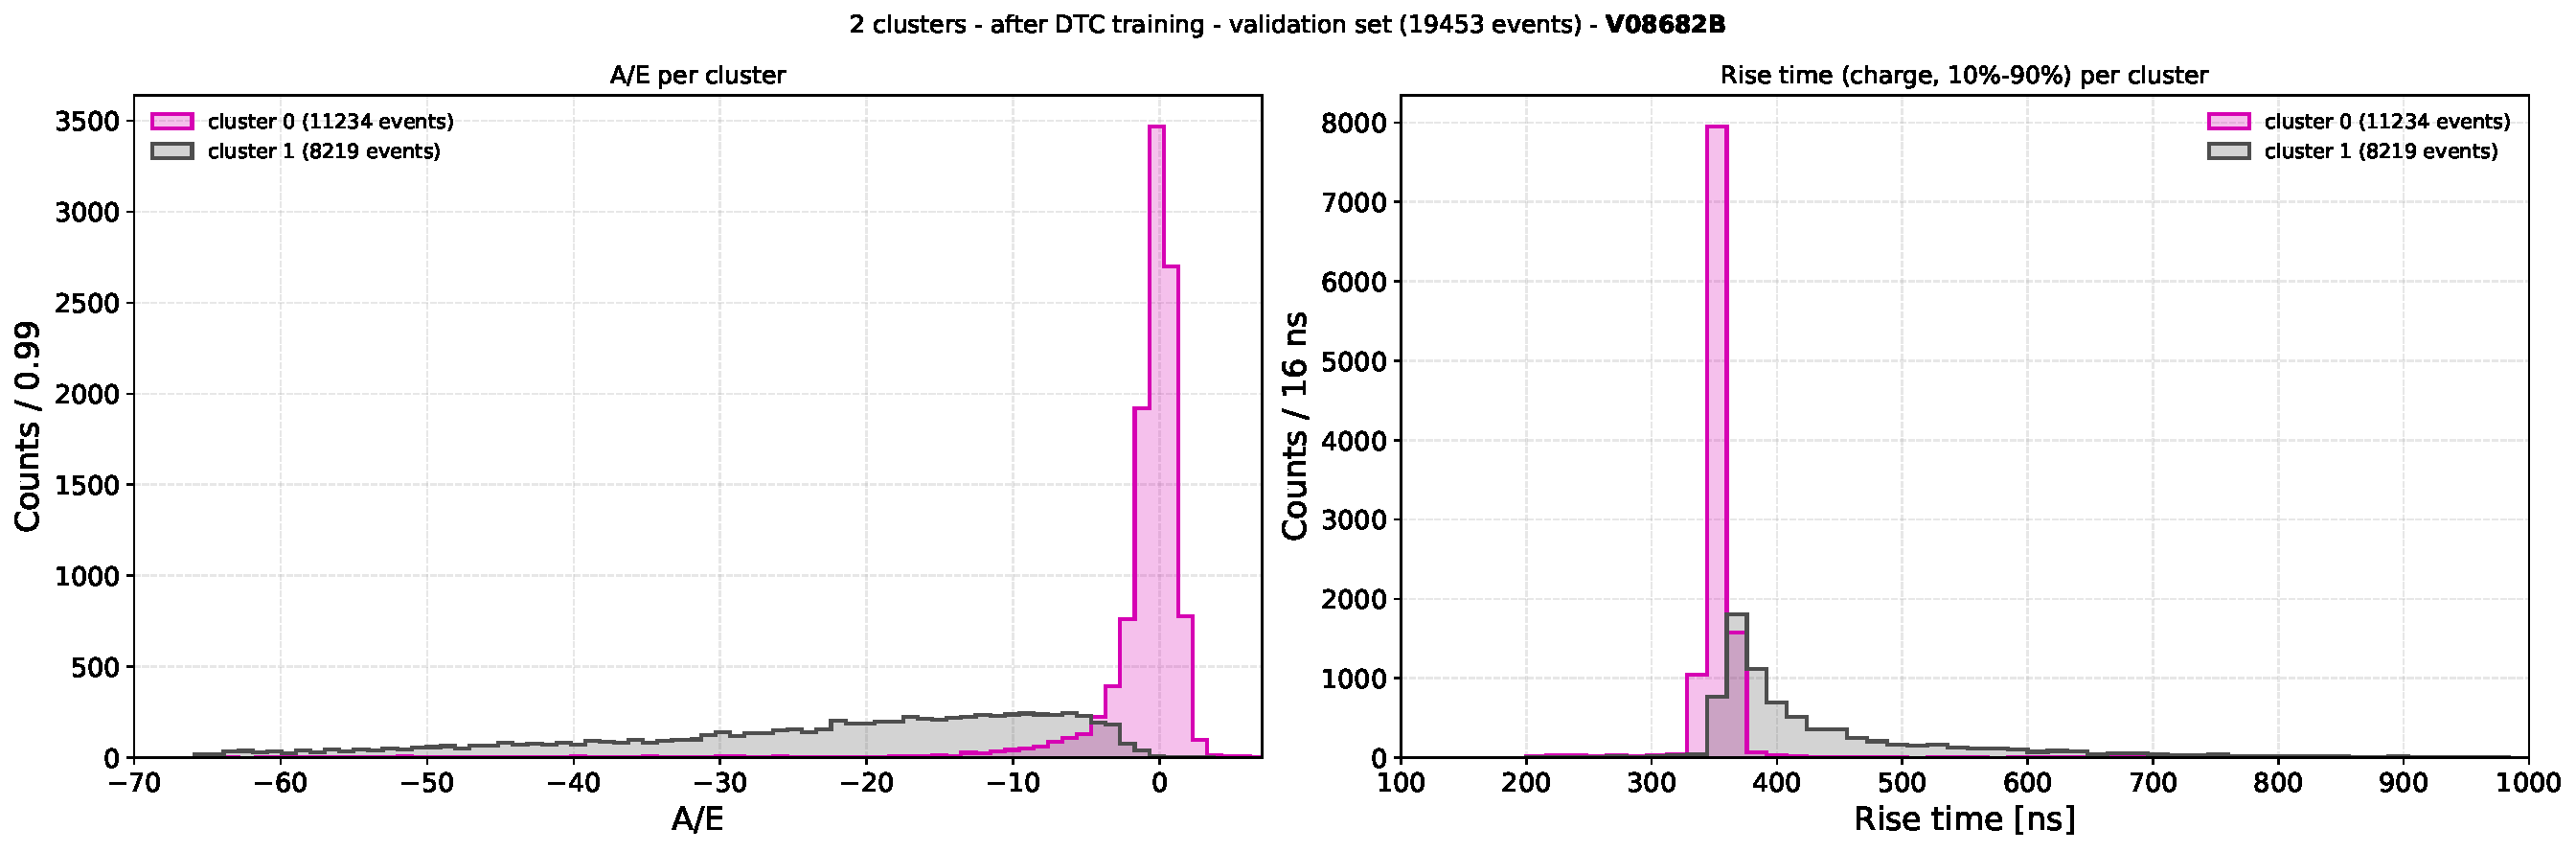
\includegraphics[width=\textwidth,height=0.27\textheight,keepaspectratio]{plots/V08682B/DTC/acf_2cl_AoE_risetime_val_linear.pdf}\\[2pt]
    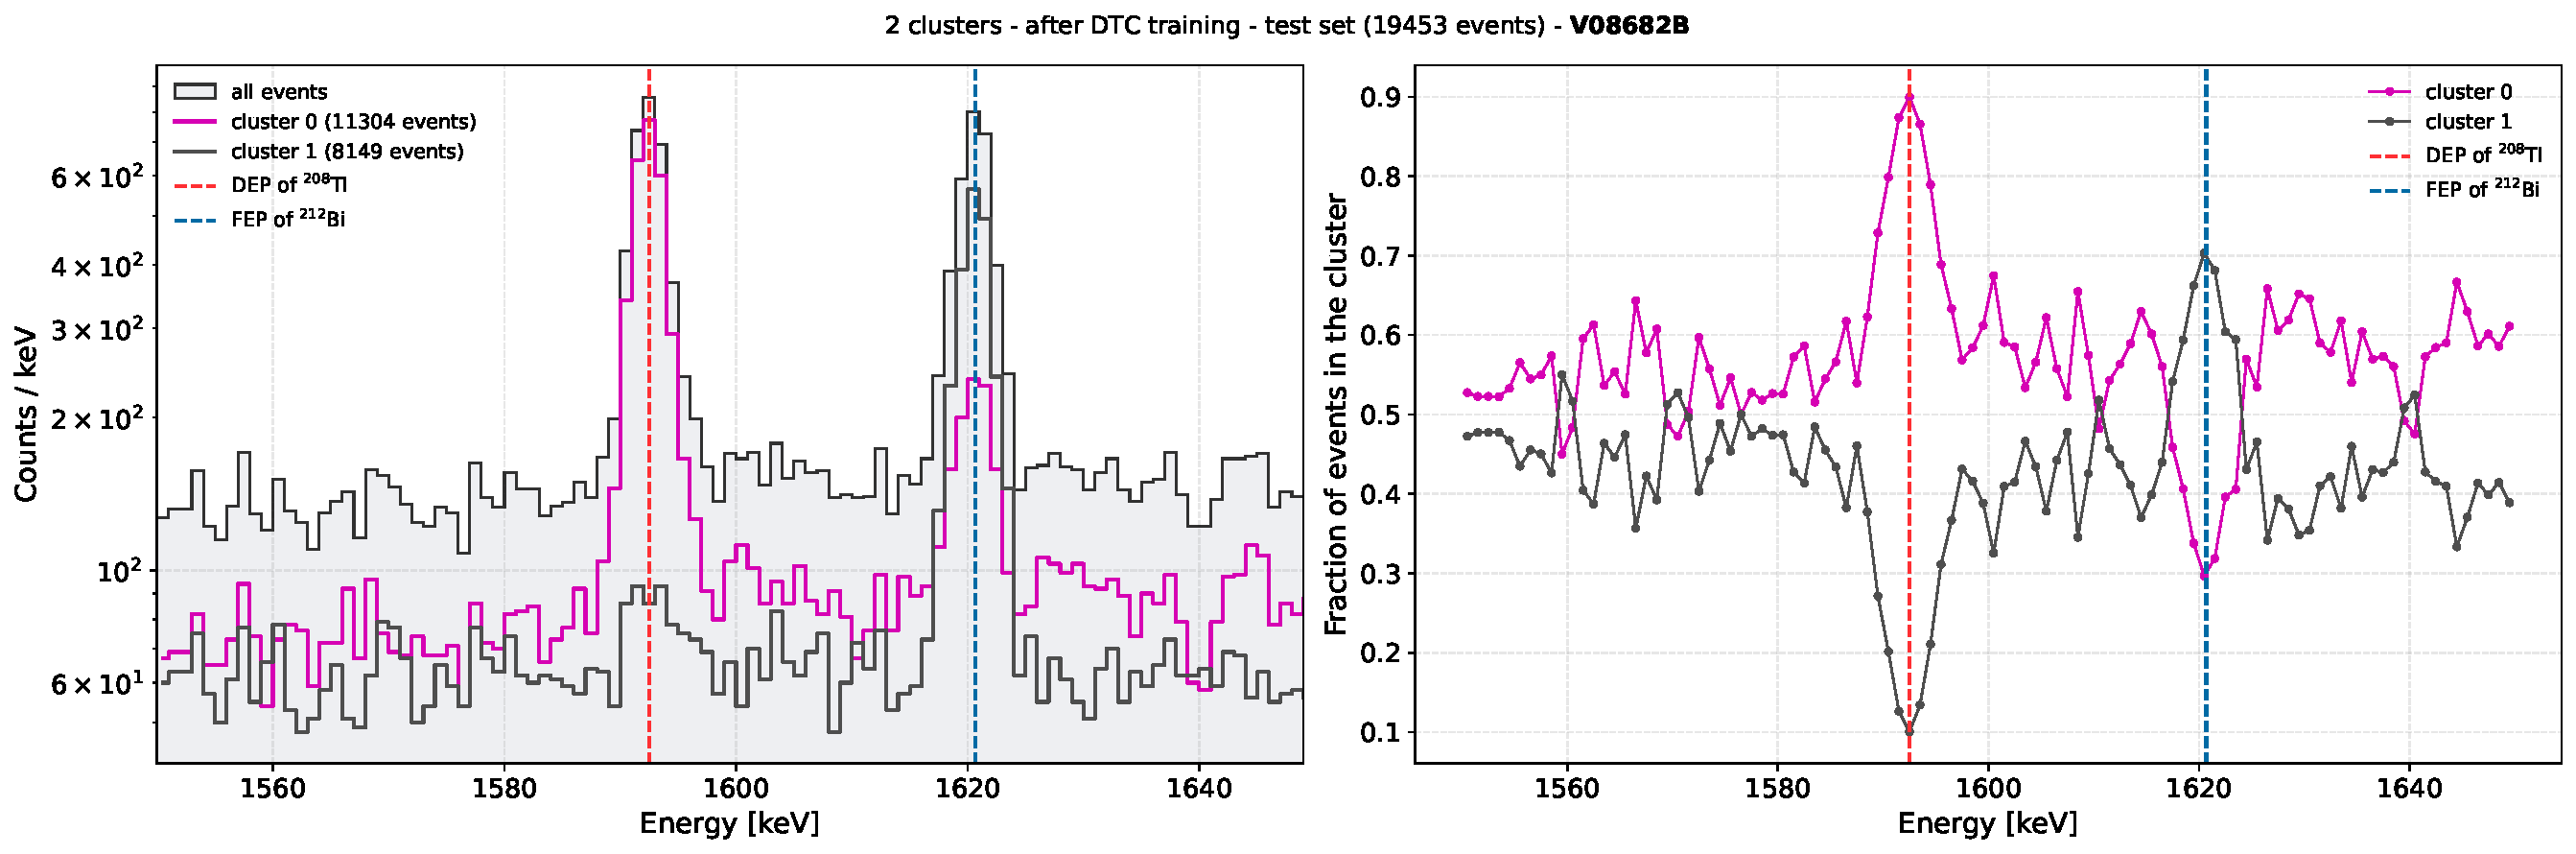
\includegraphics[width=\textwidth,height=0.27\textheight,keepaspectratio]{plots/V08682B/DTC/acf_2cl_energy_test.pdf}\\[2pt]
    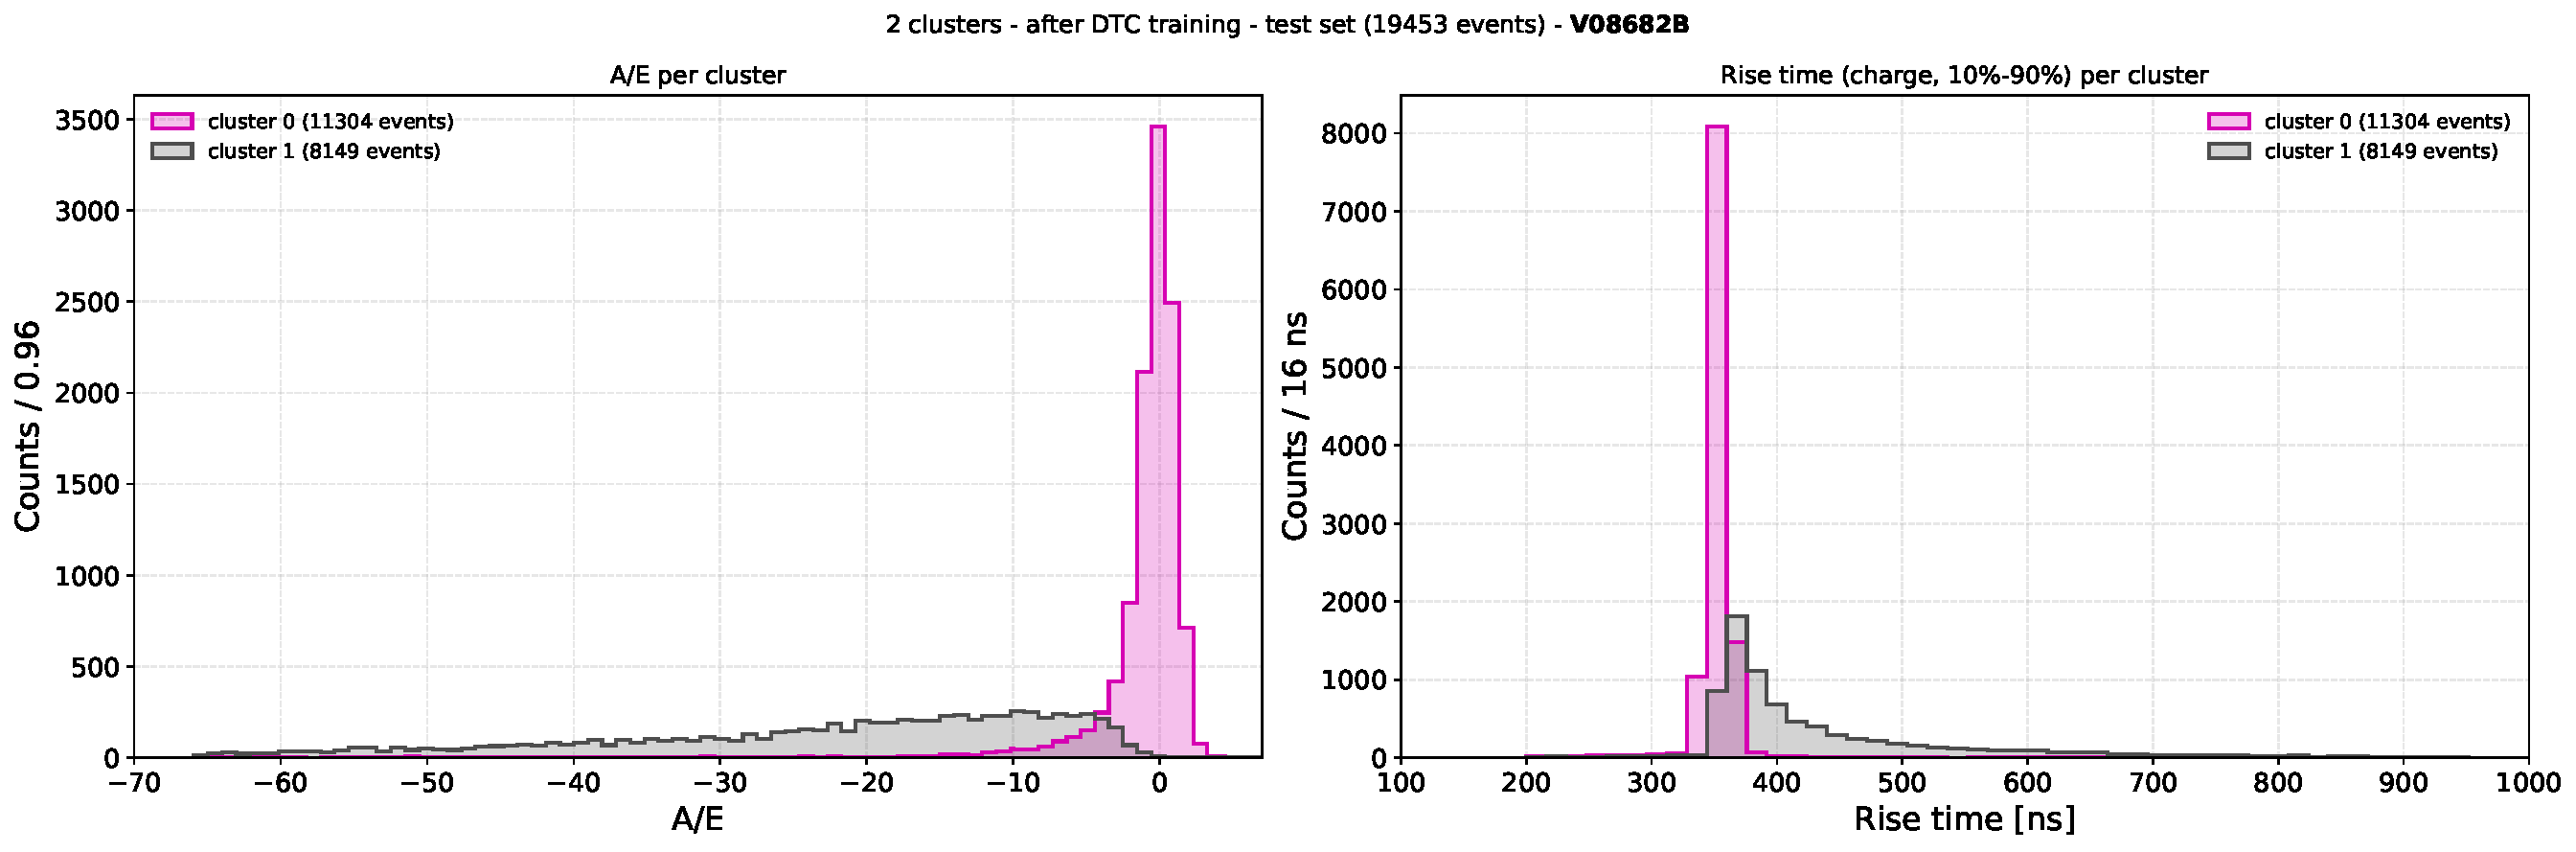
\includegraphics[width=\textwidth,height=0.27\textheight,keepaspectratio]{plots/V08682B/DTC/acf_2cl_AoE_risetime_test_linear.pdf}
    \caption{Clustering results with the \ac{ACF} metric on the validation set (first and second rows) and on the test set (third and fourth rows): energy spectrum of each cluster and fraction of events assigned to each cluster as a function of energy (first and third rows), and \ac{AE} and rise time distributions of the two clusters (second and fourth rows).}
    \label{fig:acf-aoe-V08682B}
    \label{fig:acf-aoe-train-V08682B}
    \label{fig:acf-aoe-valid-V08682B}
    \label{fig:acf-aoe-test-V08682B}
\end{figure}

\begin{figure}[H]
    \centering
    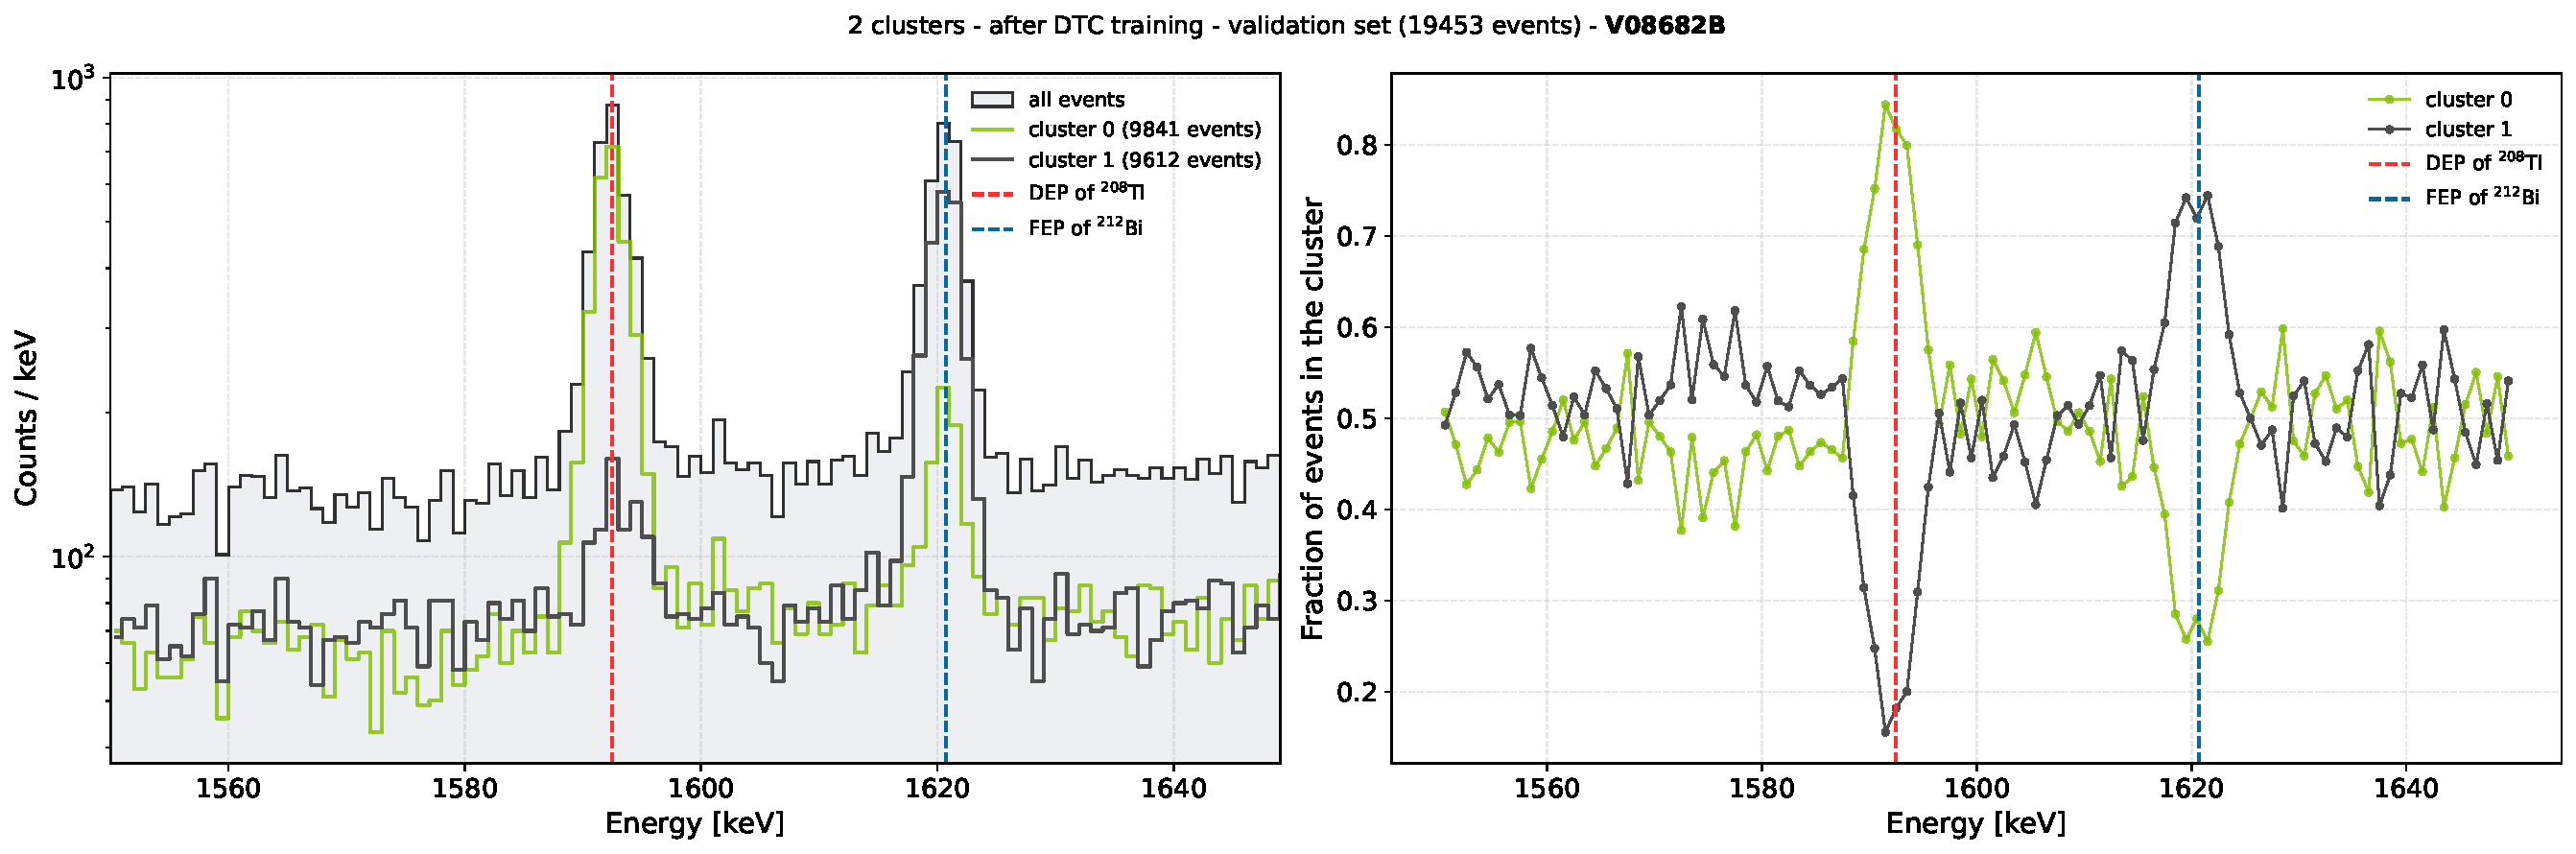
\includegraphics[width=\textwidth,height=0.27\textheight,keepaspectratio]{plots/V08682B/DTC/eucl_2cl_energy_val.pdf}\\[2pt]
    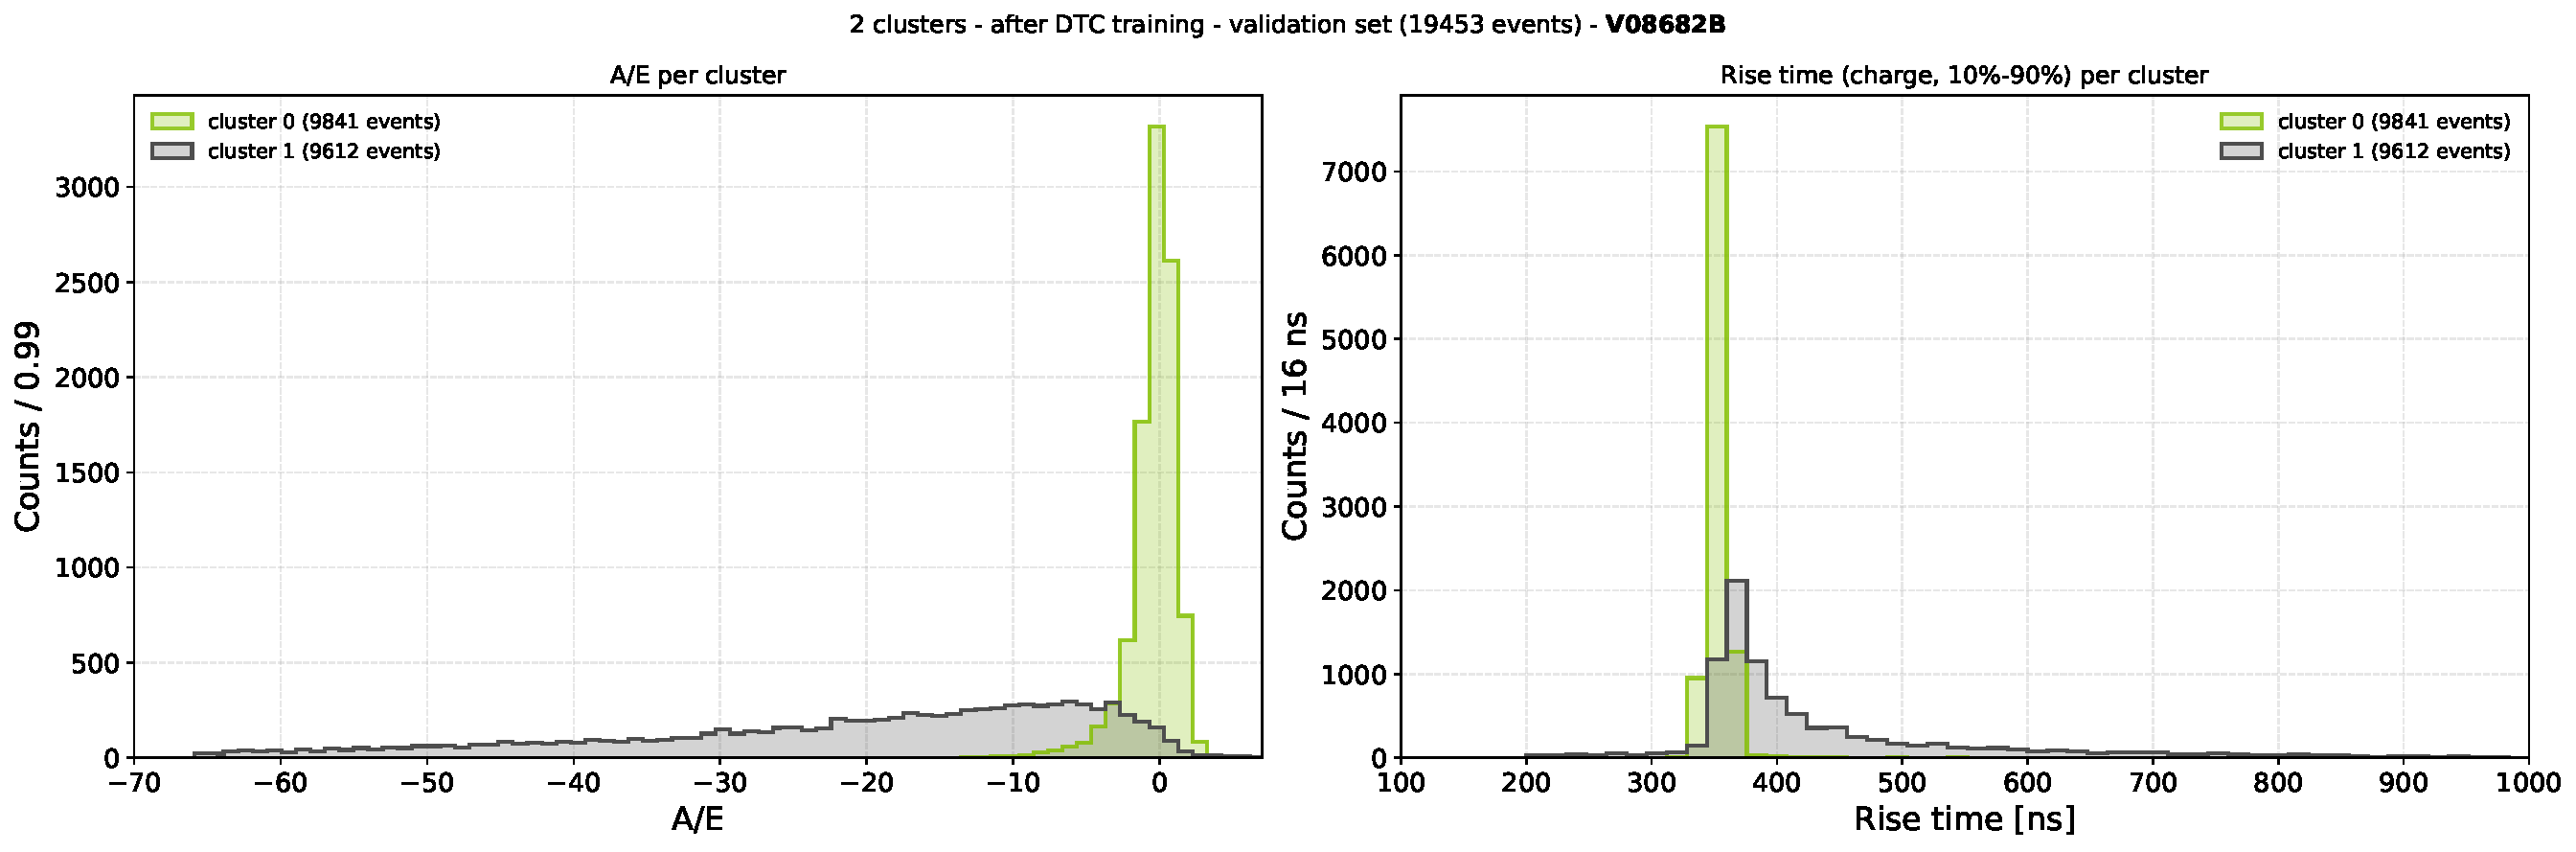
\includegraphics[width=\textwidth,height=0.27\textheight,keepaspectratio]{plots/V08682B/DTC/eucl_2cl_AoE_risetime_val_linear.pdf}\\[2pt]
    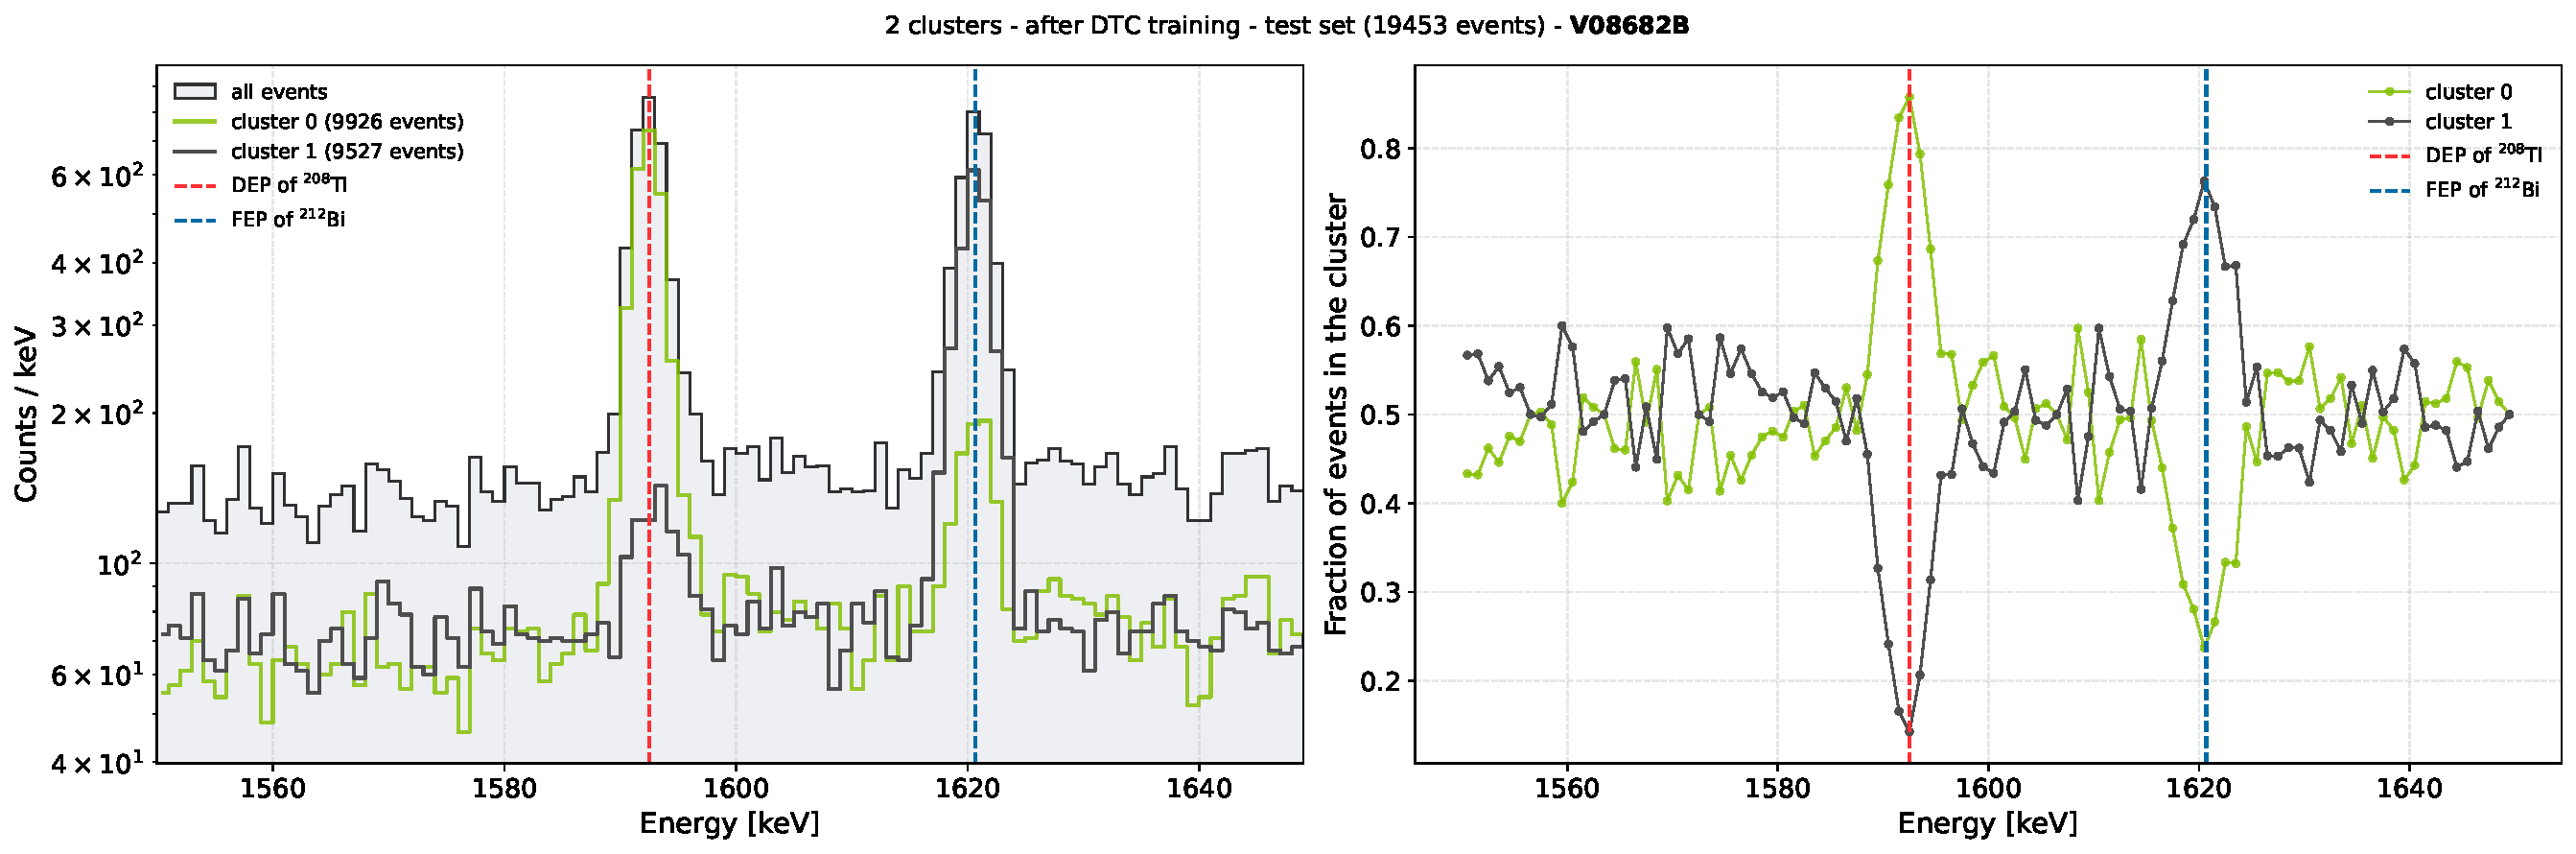
\includegraphics[width=\textwidth,height=0.27\textheight,keepaspectratio]{plots/V08682B/DTC/eucl_2cl_energy_test.pdf}\\[2pt]
    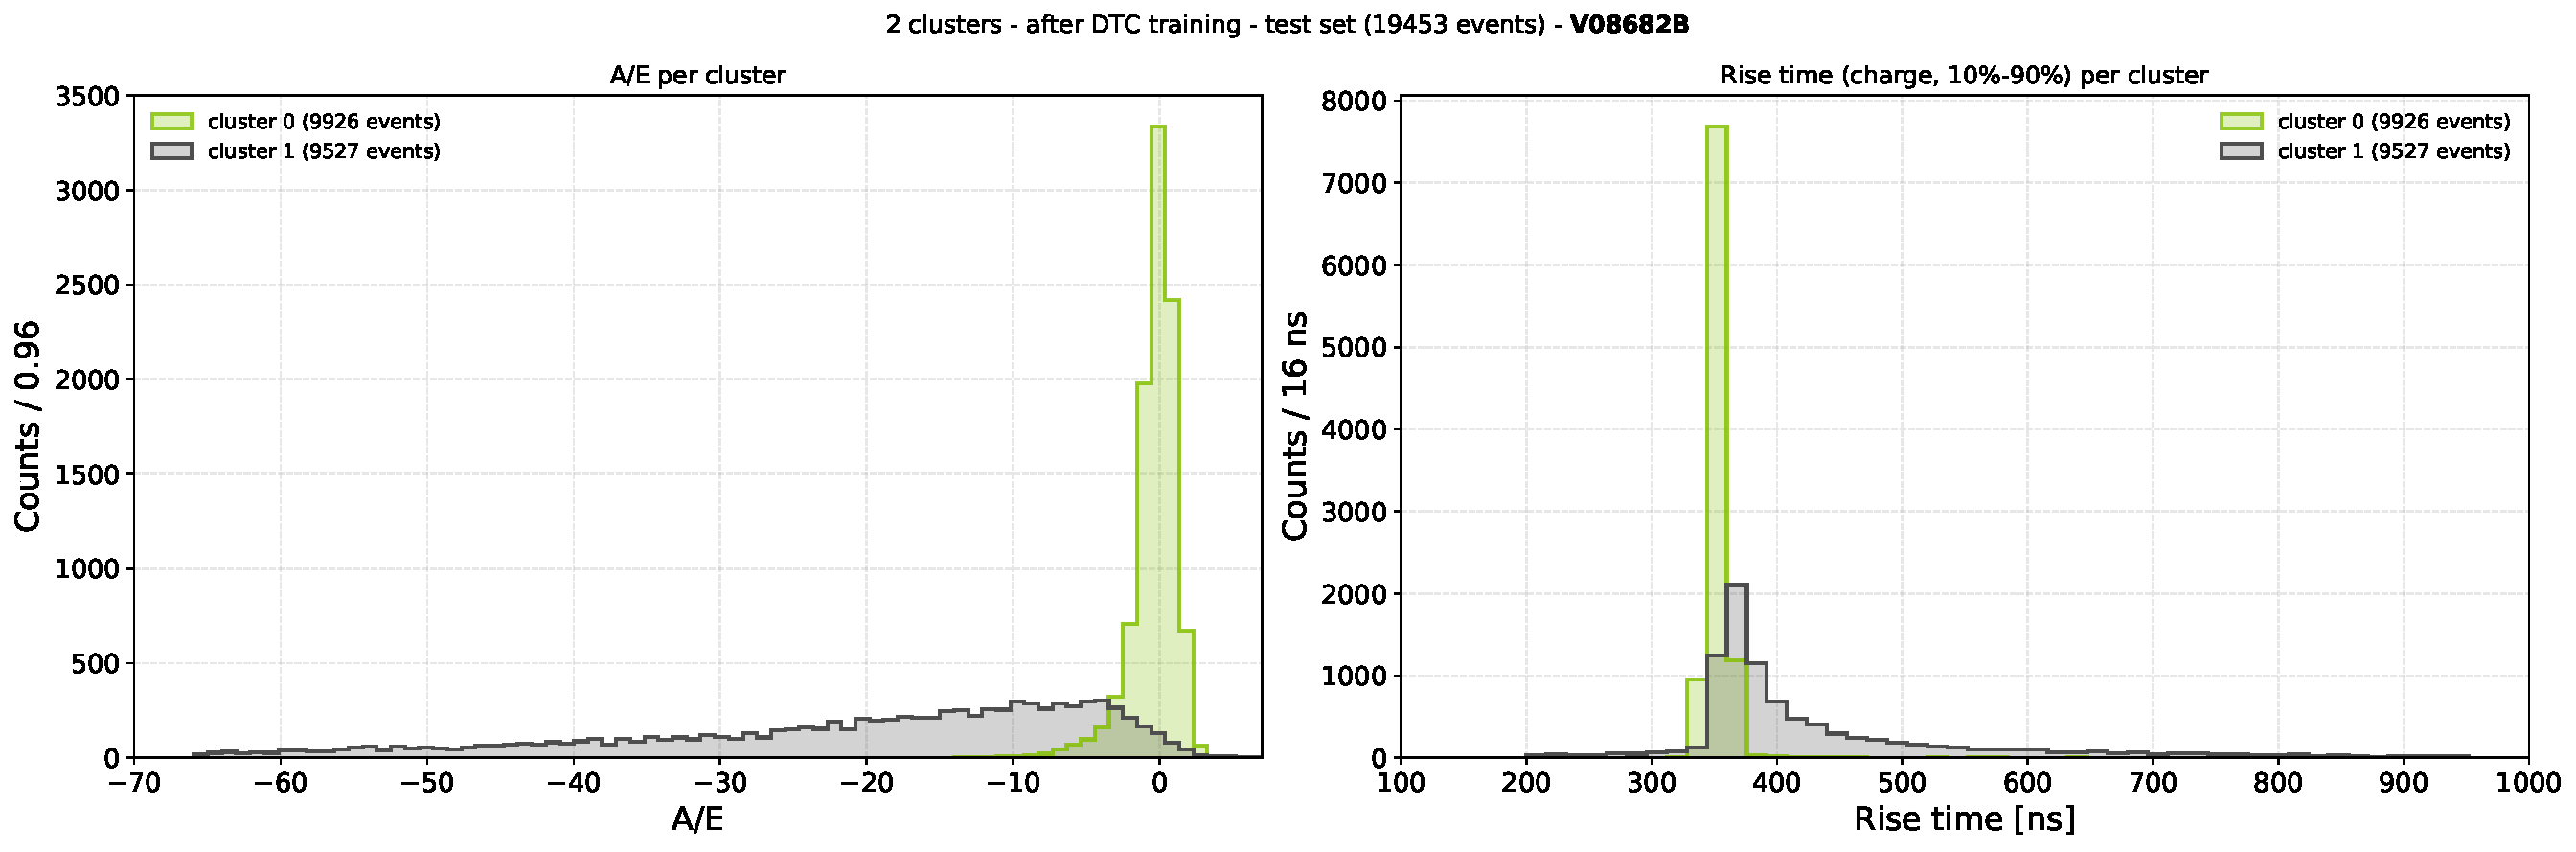
\includegraphics[width=\textwidth,height=0.27\textheight,keepaspectratio]{plots/V08682B/DTC/eucl_2cl_AoE_risetime_test_linear.pdf}
    \caption{Clustering results with the \ac{EUC} metric on the validation set (first and second rows) and on the test set (third and fourth rows): energy spectrum of each cluster and fraction of events assigned to each cluster as a function of energy (first and third rows), and \ac{AE} and rise time distributions of the two clusters (second and fourth rows).}
    \label{fig:euclidean-aoe-V08682B}
    \label{fig:euclidean-aoe-train-V08682B}
    \label{fig:euclidean-aoe-valid-V08682B}
    \label{fig:euclidean-aoe-test-V08682B}
\end{figure}

\begin{figure}[H]
    \centering
    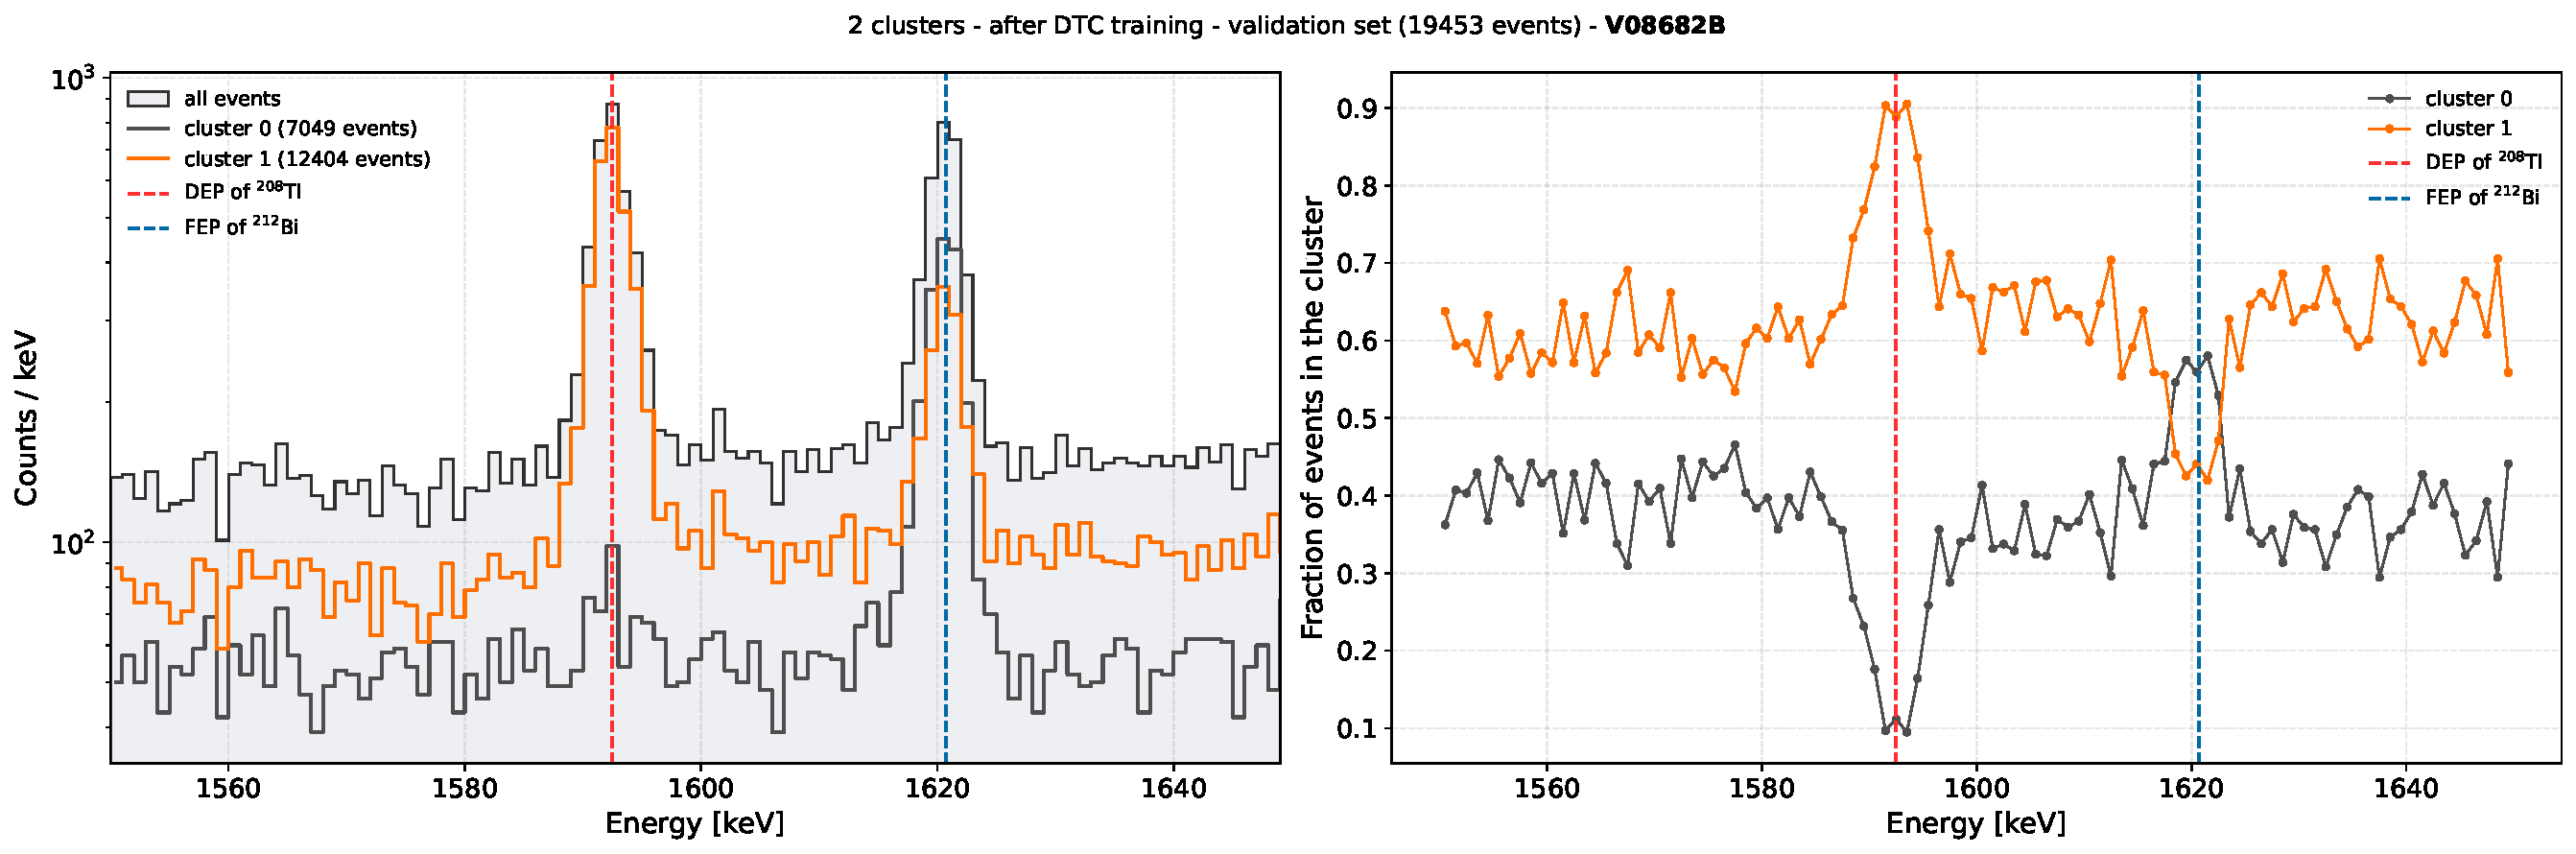
\includegraphics[width=\textwidth,height=0.27\textheight,keepaspectratio]{plots/V08682B/DTC/cid_2cl_energy_val.pdf}\\[2pt]
    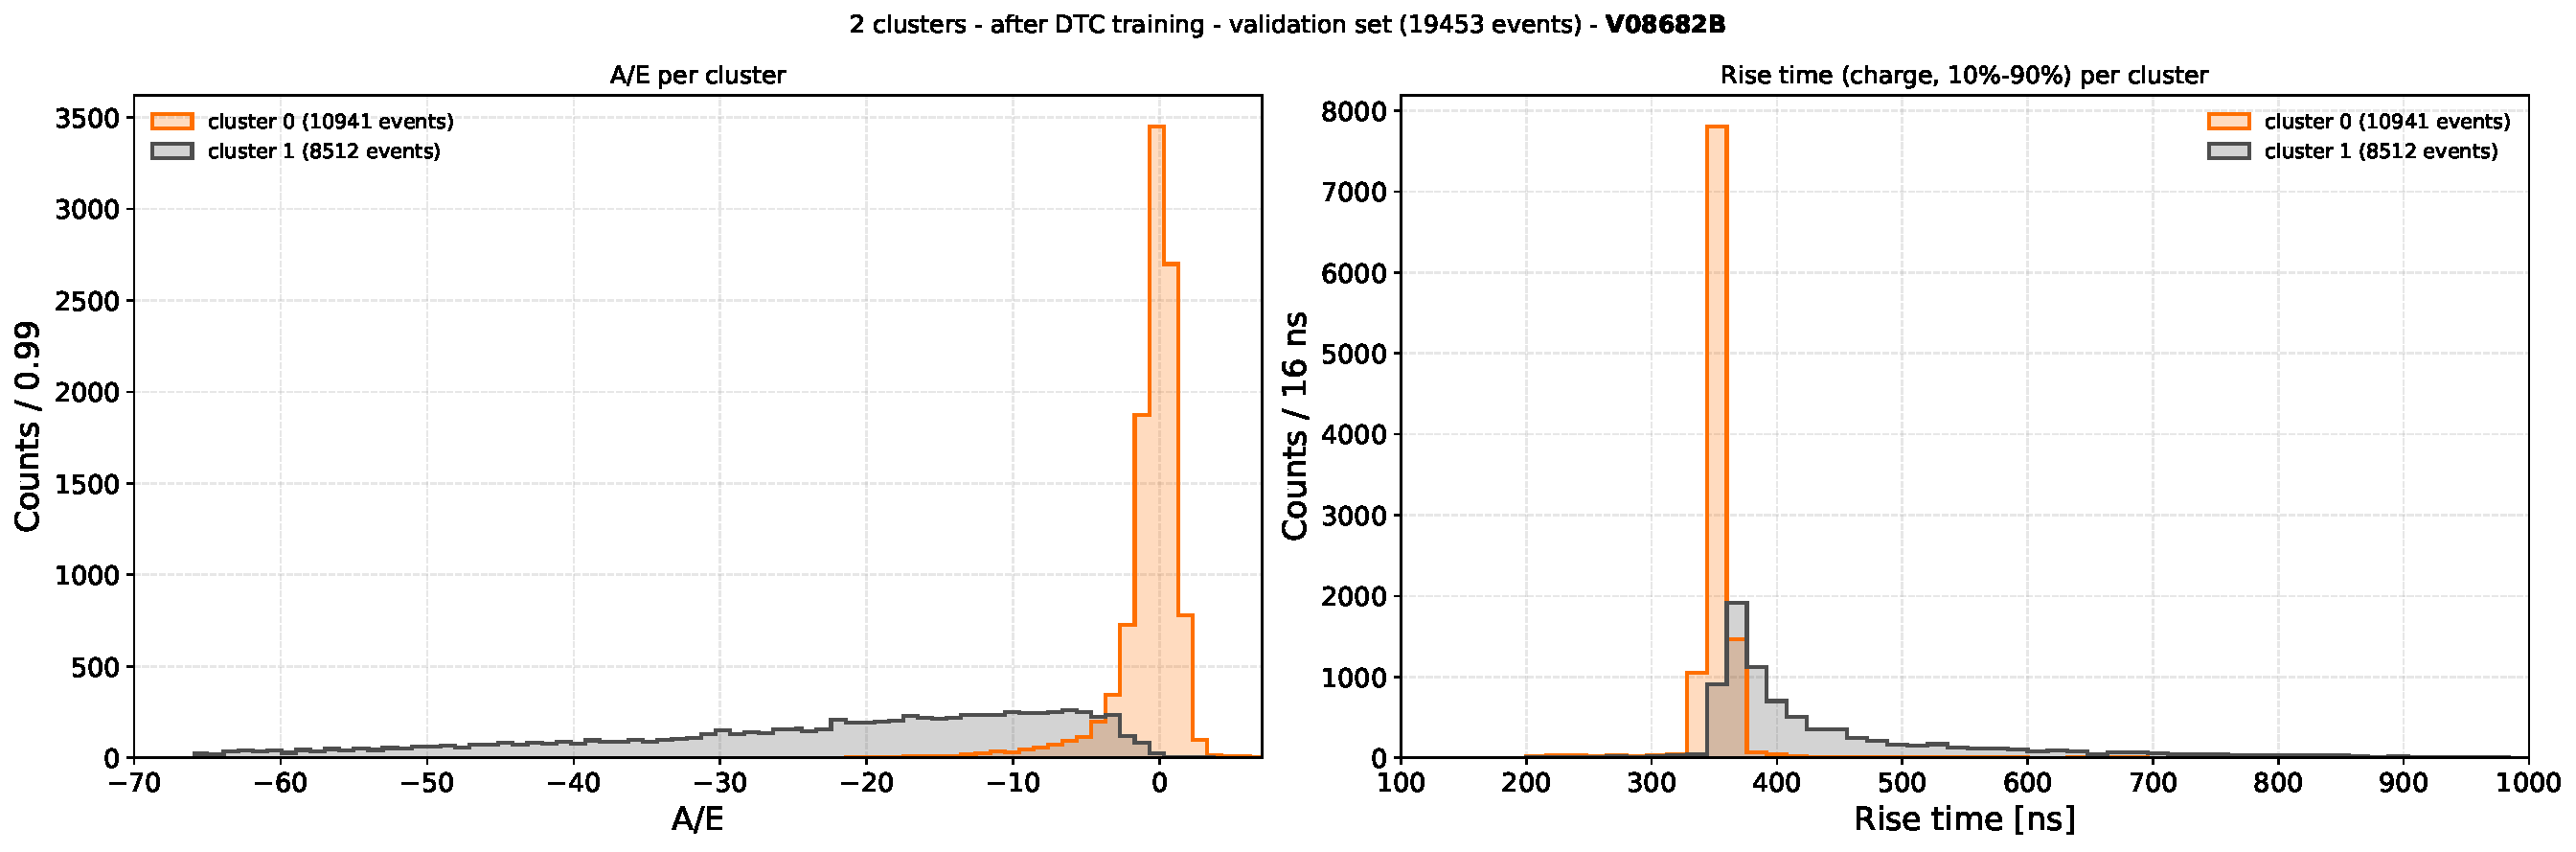
\includegraphics[width=\textwidth,height=0.27\textheight,keepaspectratio]{plots/V08682B/DTC/cid_2cl_AoE_risetime_val_linear.pdf}\\[2pt]
    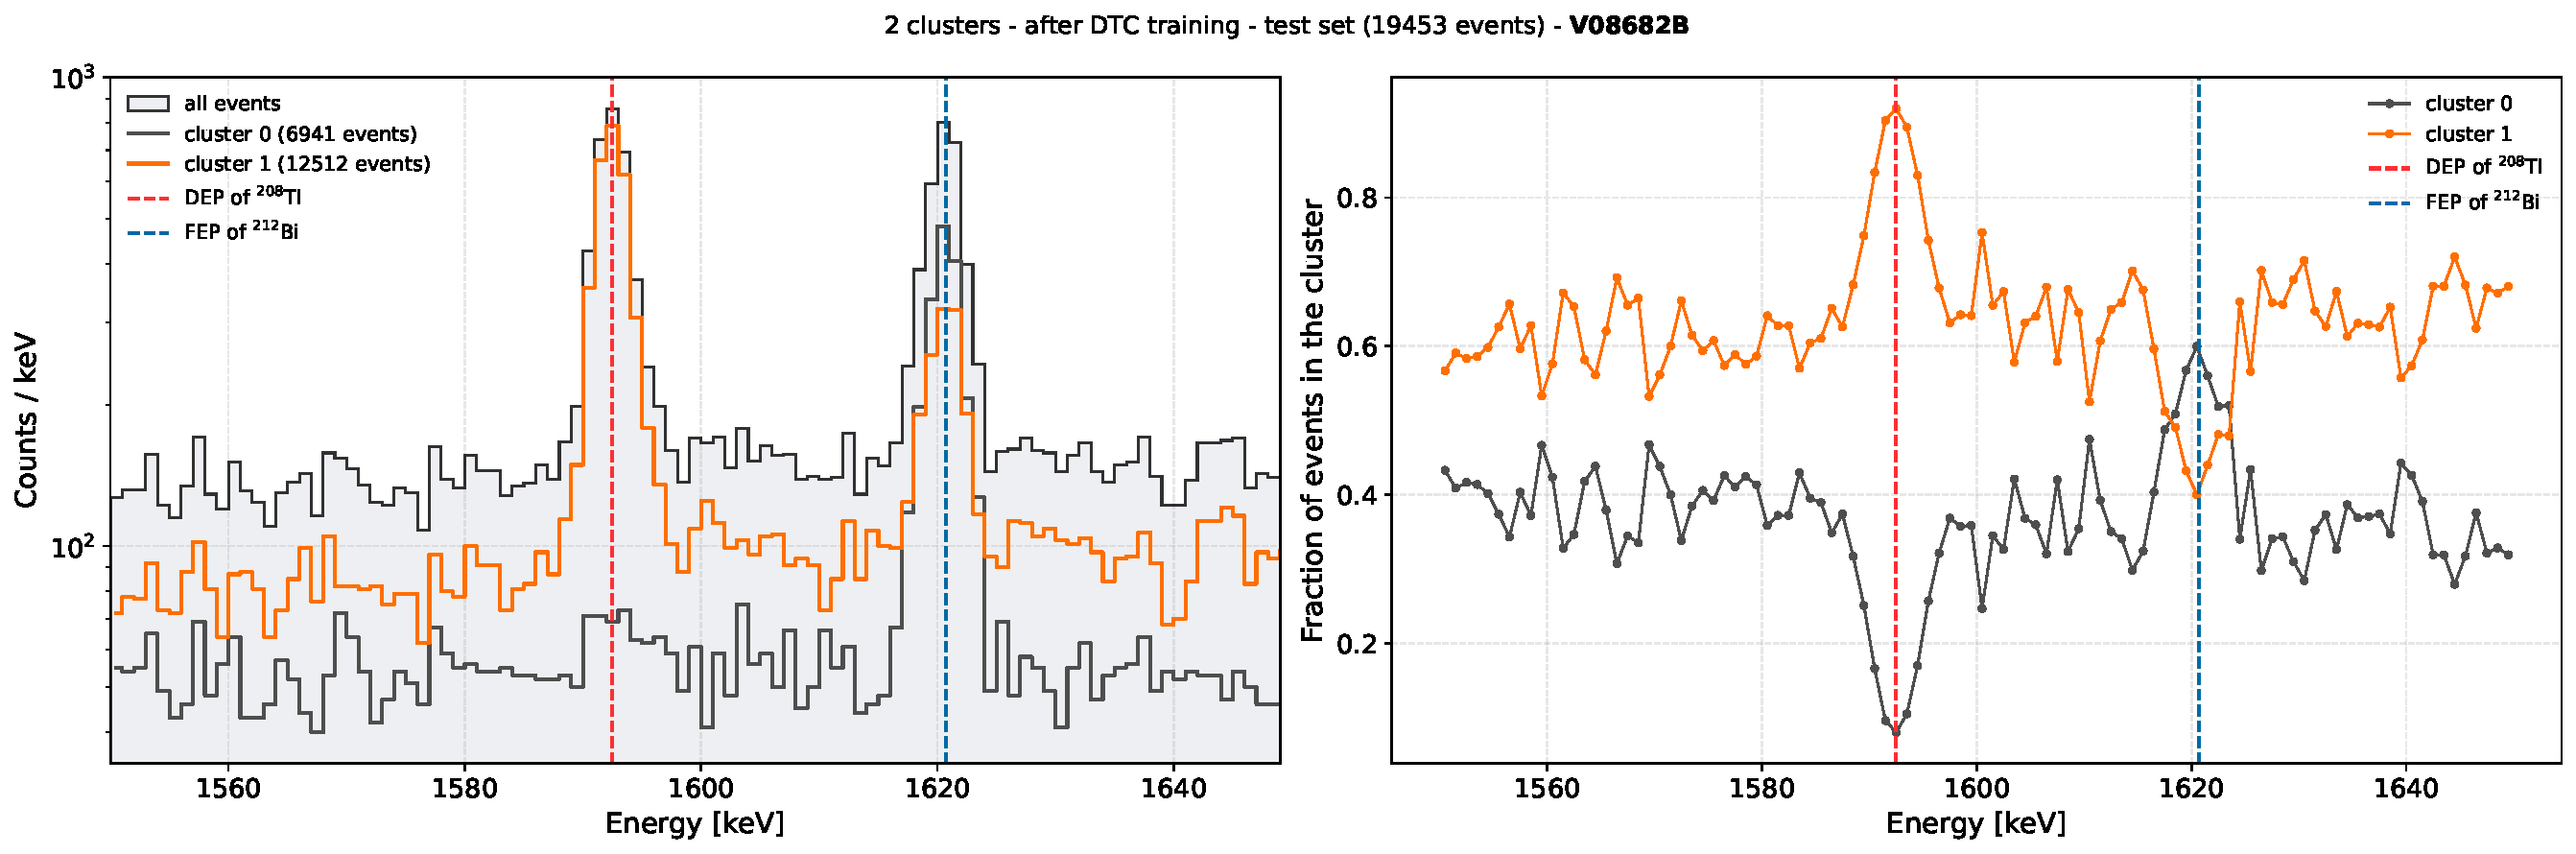
\includegraphics[width=\textwidth,height=0.27\textheight,keepaspectratio]{plots/V08682B/DTC/cid_2cl_energy_test.pdf}\\[2pt]
    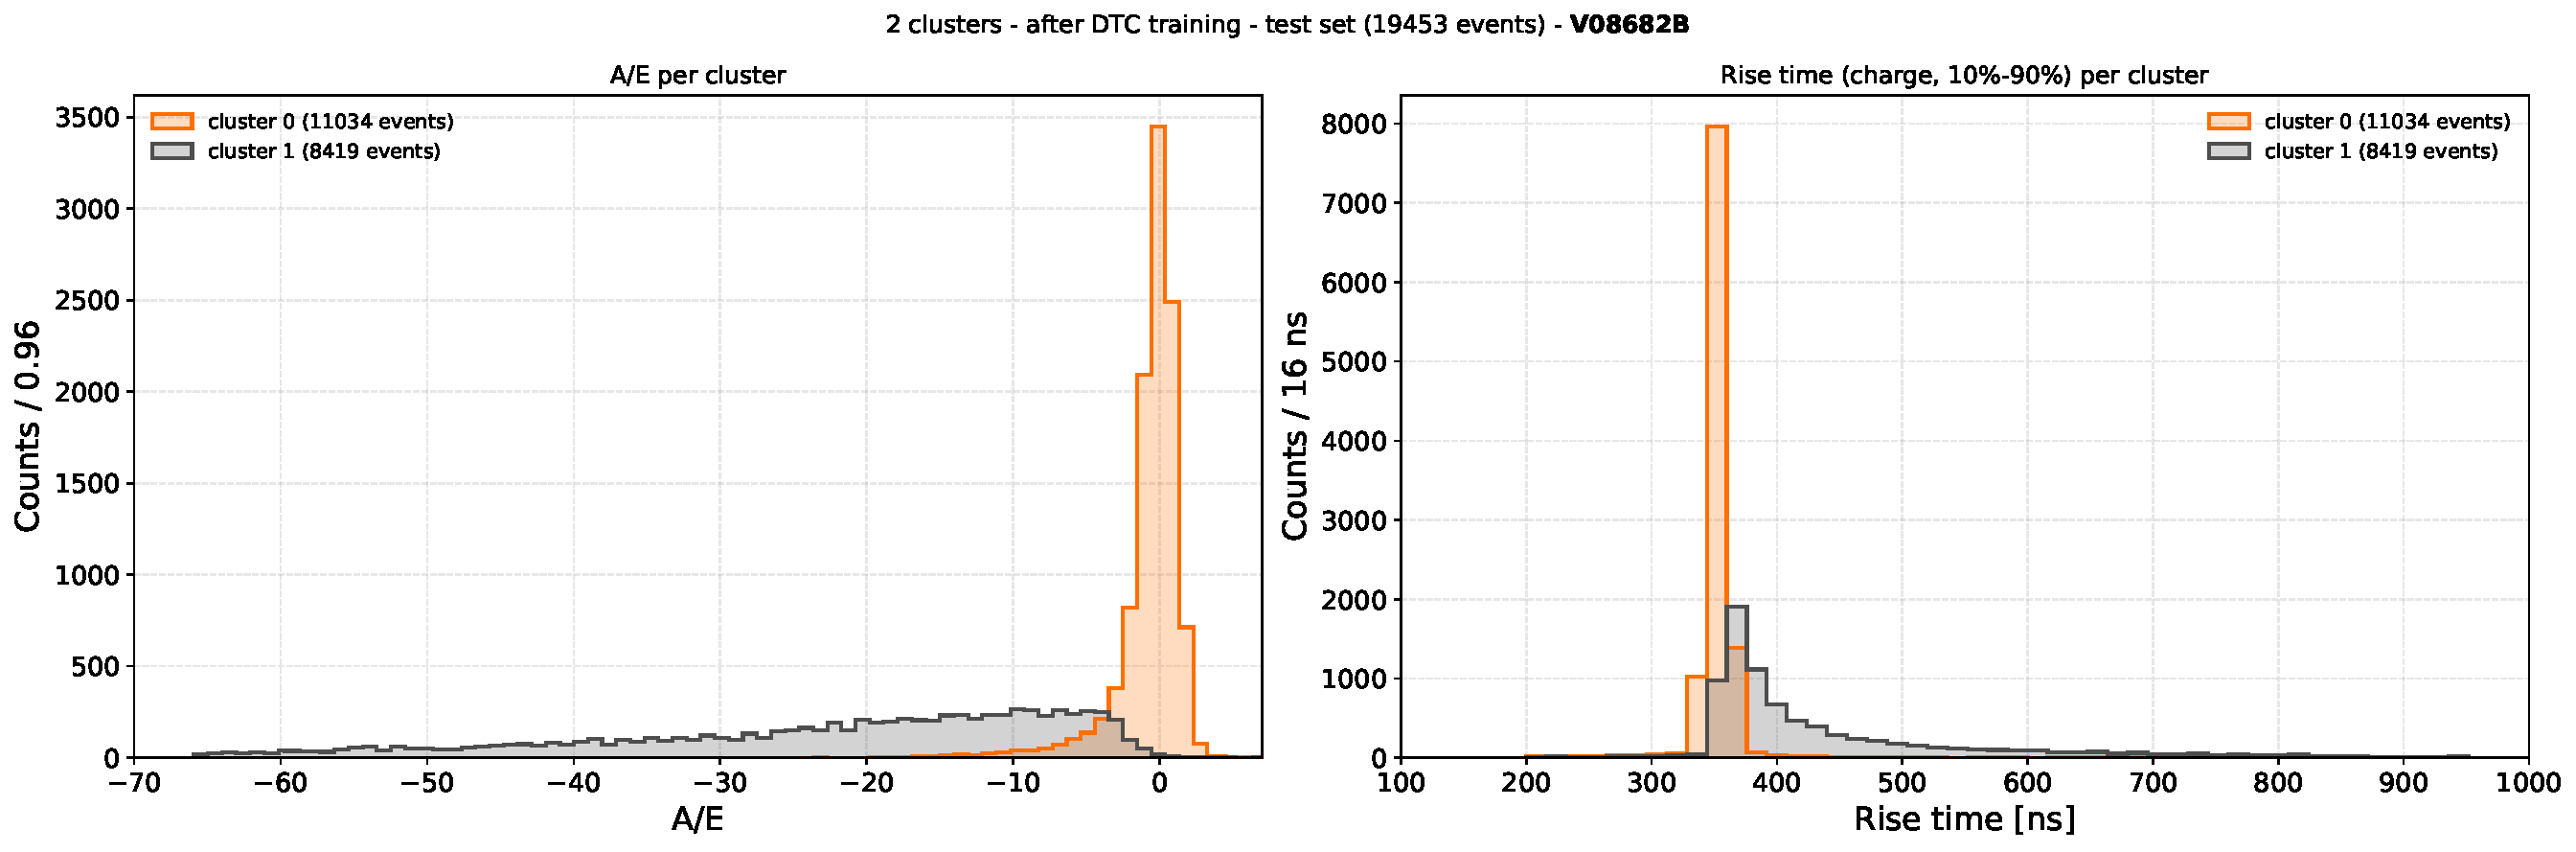
\includegraphics[width=\textwidth,height=0.27\textheight,keepaspectratio]{plots/V08682B/DTC/cid_2cl_AoE_risetime_test_linear.pdf}
    \caption{Clustering results with the \ac{CID} metric on the validation set (first and second rows) and on the test set (third and fourth rows): energy spectrum of each cluster and fraction of events assigned to each cluster as a function of energy (first and third rows), and \ac{AE} and rise time distributions of the two clusters (second and fourth rows).}
    \label{fig:cid-aoe-V08682B}
    \label{fig:cid-aoe-train-V08682B}
    \label{fig:cid-aoe-valid-V08682B}
    \label{fig:cid-aoe-test-V08682B}
\end{figure}